\documentclass{default}

\begin{document}

\tableofcontents

\chapter{Introduction}
\textit{Status: Non-functional}

This is a large project that will take a lot of well-rounded expertise in order to fully understand
and build. I will probably be able to build this without a solid understanding of how the system
works. However, if I'm able to fully understanding each step in the process I'll walk away with a
solid understanding of how to design a complicated computer system, how to build a nontrivial PCB,
and how to program raw hardware from the ground up, including the programming of an FPGA (which is
ultimately the main focus of these months).

\chapter{Schematic In-Depth Description}

\section{Power}

The power sheet receives a 12V input via a barrel jack (Figure~\ref{fig:barrel-jack}) and then
outputs various voltages and currents to feed other components in the circuit.

\begin{figure}[h]
  \centering
  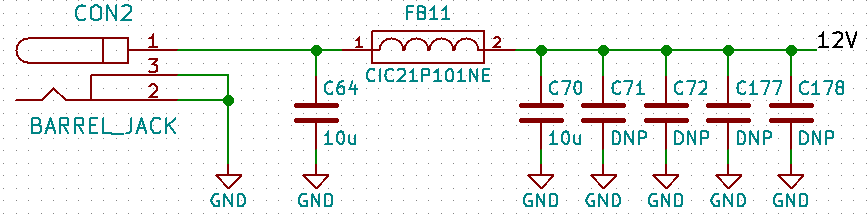
\includegraphics[width=0.9\textwidth]{data/barrel-jack.png}
  \caption{Barrel jack voltage input.}
  \label{fig:barrel-jack}
\end{figure}

The barrel jack input is filtered with a ferrite bead in a pi filter formation. This filter removes
AC components of the input voltage and prevents both external RF signals from interfering with its
operation and internally generated RF signals from radiating from it and affecting the operation of
other components in the circuit.

\begin{figure}[h]
  \centering
  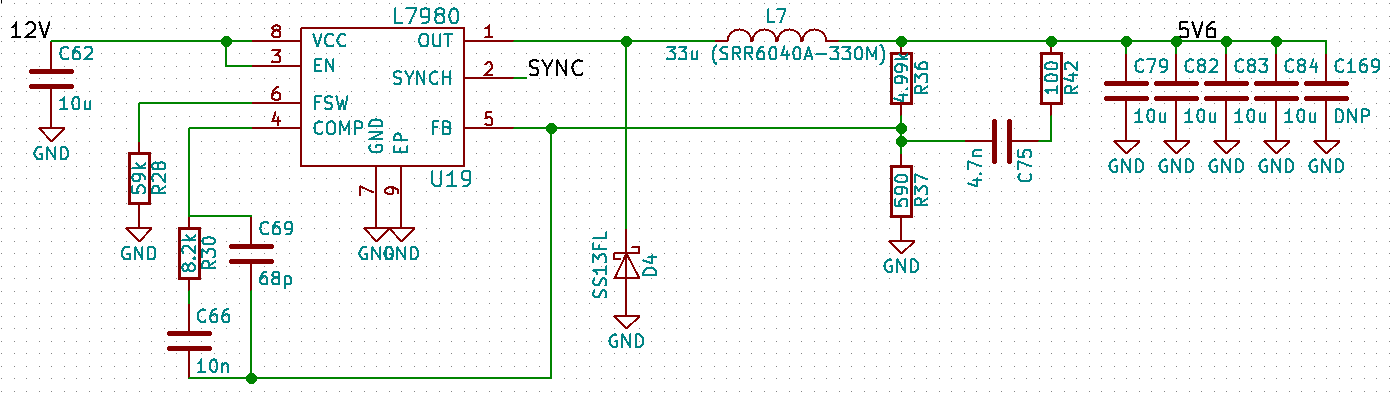
\includegraphics[width=1\textwidth]{data/buck-converter.png}
  \caption{One of the several buck converters used to derive various voltages from the 12V input
    voltage.}
  \label{fig:buck-converter}
\end{figure}

The 12V input feeds into several buck converters that output several different voltages. One such
buck converter is shown in Figure~\ref{fig:buck-converter}. The input 10 $\mu F$ capacitor is
specified by the data sheet. The EN pin is connected to the power source because a voltage higher
than 1.2V powers on the device (ours is 12V) and a voltage lower than 0.3V powers it off. The
$F_{\text{SW}}$ pin is used to set the switching frequency of the buck converter. If it is left
free-floating, the switching frequency will be 250kHz. However, we can adjust the switching
frequency by attaching it to a resistor to ground. The equation for doing so is:

\begin{equation}
  R_{\text{SW}}=\frac{28.5\times 10^9}{F_{\text{SW}}-250\times 10^3}-3.23\times 10^3
\end{equation}

So, the resistor value of $\text{59k$\ohm$}$ in the schematic corresponds to a switching frequency
of 708kHz. A higher switching frequency allows a lower minimum inductance value, which decreases the
cost of a circuit ($L_{\text{min}}\propto 1/F_{\text{SW}}$). To select an inductor value, we use
Equation~\ref{eq:L-select-eqn}.

\begin{equation}
  \Delta I_{\text{L}} = \frac{V_{\text{IN}}-V_{\text{OUT}}}{L} T_{\text{ON}}
  \label{eq:L-select-eqn}
\end{equation}

The duty cycle is given by Equation~\ref{eq:duty-cycle-eqn}. Since $V_{\text{IN}} = 12V$ and
$V_{\text{OUT}} = 5.6V$, $D = 47\%$. We already found that the switching frequency is 708kHz, which
gives a total period of $1. 41\mu \text{s}$ and therefore $t_{\text{ON}} = 0.659\mu \text{s}$. The
inductor value used is $33\mu \text{H}$ which gives a current ripple of 128mA. The max current draw
is expected to be about 300mA, given the max power (1.6W) of
\href{http://www.analog.com/media/en/technical-documentation/data-sheets/ADL5802.pdf}{ADL5802} for
an operation at 5.5V (ours will actually operate at 5V and I expect the power dissipation to go down
proportionally). This puts the ripple current at just over 40\% of the max current draw, which seems
high. I would have expected the current ripple to be contained to about 10\% of max current draw,
which would put the inductor value at $211\mu\text{H}$.

\begin{equation} DV_{\text{IN}} = V_{\text{OUT}}
  \label{eq:duty-cycle-eqn}
\end{equation}

It is worth noting that the inductor in this buck converter is not included within the device
itself. Instead, we must attach or own. The Schottky diode is a flyback diode that prevents a
voltage spike across the switch inside the device. A Schottky diode is used instead of a traditional
diode since it has a lower forward voltage drop and will therefore cause a lower voltage drop across
the inductor, which will cause it to lose stored energy less quickly.

This device uses a voltage-mode PWM comparator to stabilize the output voltage at the desired output
voltage. This is a bit technical, but all we need to know to operate the device is that the
comparison voltage is 0.6V. So, we create a voltage divider to generate a output voltage to feed
back into the FB pin which will be 0.6V when we have our desired output voltage, which is 5.6V. From
the voltage divider equation and using the resistors in the schematic (Equation~\ref{eq:fb-in}), we
see that the voltage input to FB is indeed close to 0.6V.

\begin{equation}
  5.6V \frac{590\Omega}{590\Omega + 4990\Omega} = 0.592V \label{eq:fb-in}
\end{equation}

The COMP pin is used to provide feedback to the error amplifier, which in turn generates the error
voltage signal that is compared with the internal sawtooth signal to determine the pulse modulation
that controls the voltage output. There are two different compensation networks that we can use, as
described in the datasheet: type II compensation and type III compensation. The datasheet recommends
the use of type III compensation for MLCC capacitors given their low ESR. \textbf{\{START
  INCOMPLETE\}} The actual calculation of these values is tricky and requires knowledge of feedback
and op-amps, which in turn requires prerequisite knowledge of transistors. I believe it's probably
necessary to complete chapters 1-4 of the Art of Electronics to understand this, so I intend to come
back to it. On the upside, this should provide a solid background for DSP \textbf{\{END
  INCOMPLETE\}}.

The buck converter outputs feed into several different chips, the first of which is an LDO regulator
for which an example is shown in Figure~\ref{fig:linear-reg}. The reason for attaching an LDO
regulator in series with a buck converter may be to reduce the noise of the circuit and increase the
efficiency at the expense of board area and cost. Particularly, the
\href{http://www.ti.com/lit/ds/symlink/tps7a91.pdf}{LDO regulator} should be able to smooth out the
noise caused by using an inductor with a low value in the buck converter. It is meant to effectively
reject noise from the input source over the frequency range of 10Hz to 10MHz. Since the switching
frequency of the buck converter is less than 1MHz and consequently the current/voltage ripple should
be of the same frequency, the LDO regulator should be sufficient to smooth out the input noise
provided, however, that it does not dip below the output voltage of the LDO regulator since the
margin for error is small. $V_{\text{IN}}-V_{\text{OUT}}=0.6V$ and linear regulators are not able to
output a voltage greater than their input voltage. The max dropout of the LDO is 0.2V, which allows
the output voltage of the buck converter a deviation of 0.4V.

\begin{figure}[h]
  \centering
  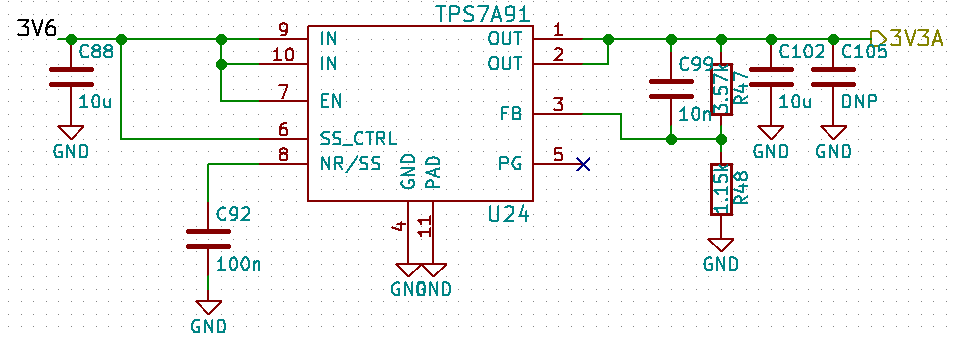
\includegraphics[width=0.75\textwidth]{data/linear-reg.png}
  \caption{A LDO regulator that takes as an input the voltage from one of the buck converters and
    whose output is directly used to drive the operation of one of the ICs elsewhere in the
    circuit.}
  \label{fig:linear-reg}
\end{figure}

The input voltage is connected to both IN pins with a bypass capacitor of 10 $\mu$F, which is the
minimum specified by the datasheet. It is additionally connected to the EN pin which activates the
LDO; the LDO is active for $V_{\text{EN}} \geq V_{\text{IH}}$ and disabled for
$V_{\text{EN}} \leq V_{\text{IL}}$ (connecting the same input to IN and EN will make
$V_{\text{EN}} = V_{\text{IH}}$, thus satisfying the first condition). The 2 resistors attached to
OUT and FB make a voltage divider that determines the output voltage of the linear regulator,
according to Equation~\ref{eq:linear-reg-vout}.

\begin{equation}
  R_1 = R_2\left(\frac{V_{\text{OUT}}}{V_{\text{REF}}}-1\right) \label{eq:linear-reg-vout}
\end{equation}

Where $V_{\text{REF}} = 0.8V$ Specifically, 1.15k and 3.57k are specified in the datasheet in order
to get an output voltage of 3.3V. SS\_CTRL is connected to IN instead of GND which increases the
soft-startup charging current to 100 $\mu$A from 6.2 $\mu$A and decreases the start-up time, which
is given by Equation~\ref{eq:linear-reg-startup-time}.

\begin{align}
  t_{\text{SS}} &= (V_{\text{REF}} \times C_{\text{NR/SS}}) /
                  I_{\text{NR/SS}} \label{eq:linear-reg-startup-time} \\
                &= 0.8V \times 100 \times 10^{-9} F/(100 \times 10^{-6} A) \\
                &= 0.8\text{ms}
\end{align}

An output capacitor of 10 $\mu$F is chosen which is the minimum specified by the
datasheet. Additionally, a feed-forward capacitor of 10nF is added between the OUT and FB pins to
improve the noise and PSRR performance of the voltage regulator. The value is recommended by the
datasheet. The $C_{\text{NR/SS}}$ capacitor of 100nF is used to create an output RC filter for
output noise and is also used to set the soft-start time. A value of between 10nF and 10$\mu$F is
recommended. PAD and GND should both be connected to ground, as indicated by the datasheet. PG
indicates whether the output voltage is in a usable state. Since we are not using it, it can be left
floating.

Another buck converter output feeds into the input of an ultra low LDO, with a dropout voltage of
40mV as shown in Figure~\ref{fig:ldo-ldo-connection}. R104 acts as a pull-up resistor, pulling the
voltage on EN high when PG is not driven. However, when PG is low, EN will be driven low. The bypass
pin is left open, although a 1$\mu$F capacitor could have been placed there to reduce output noise.

\begin{figure}[h]
  \centering
  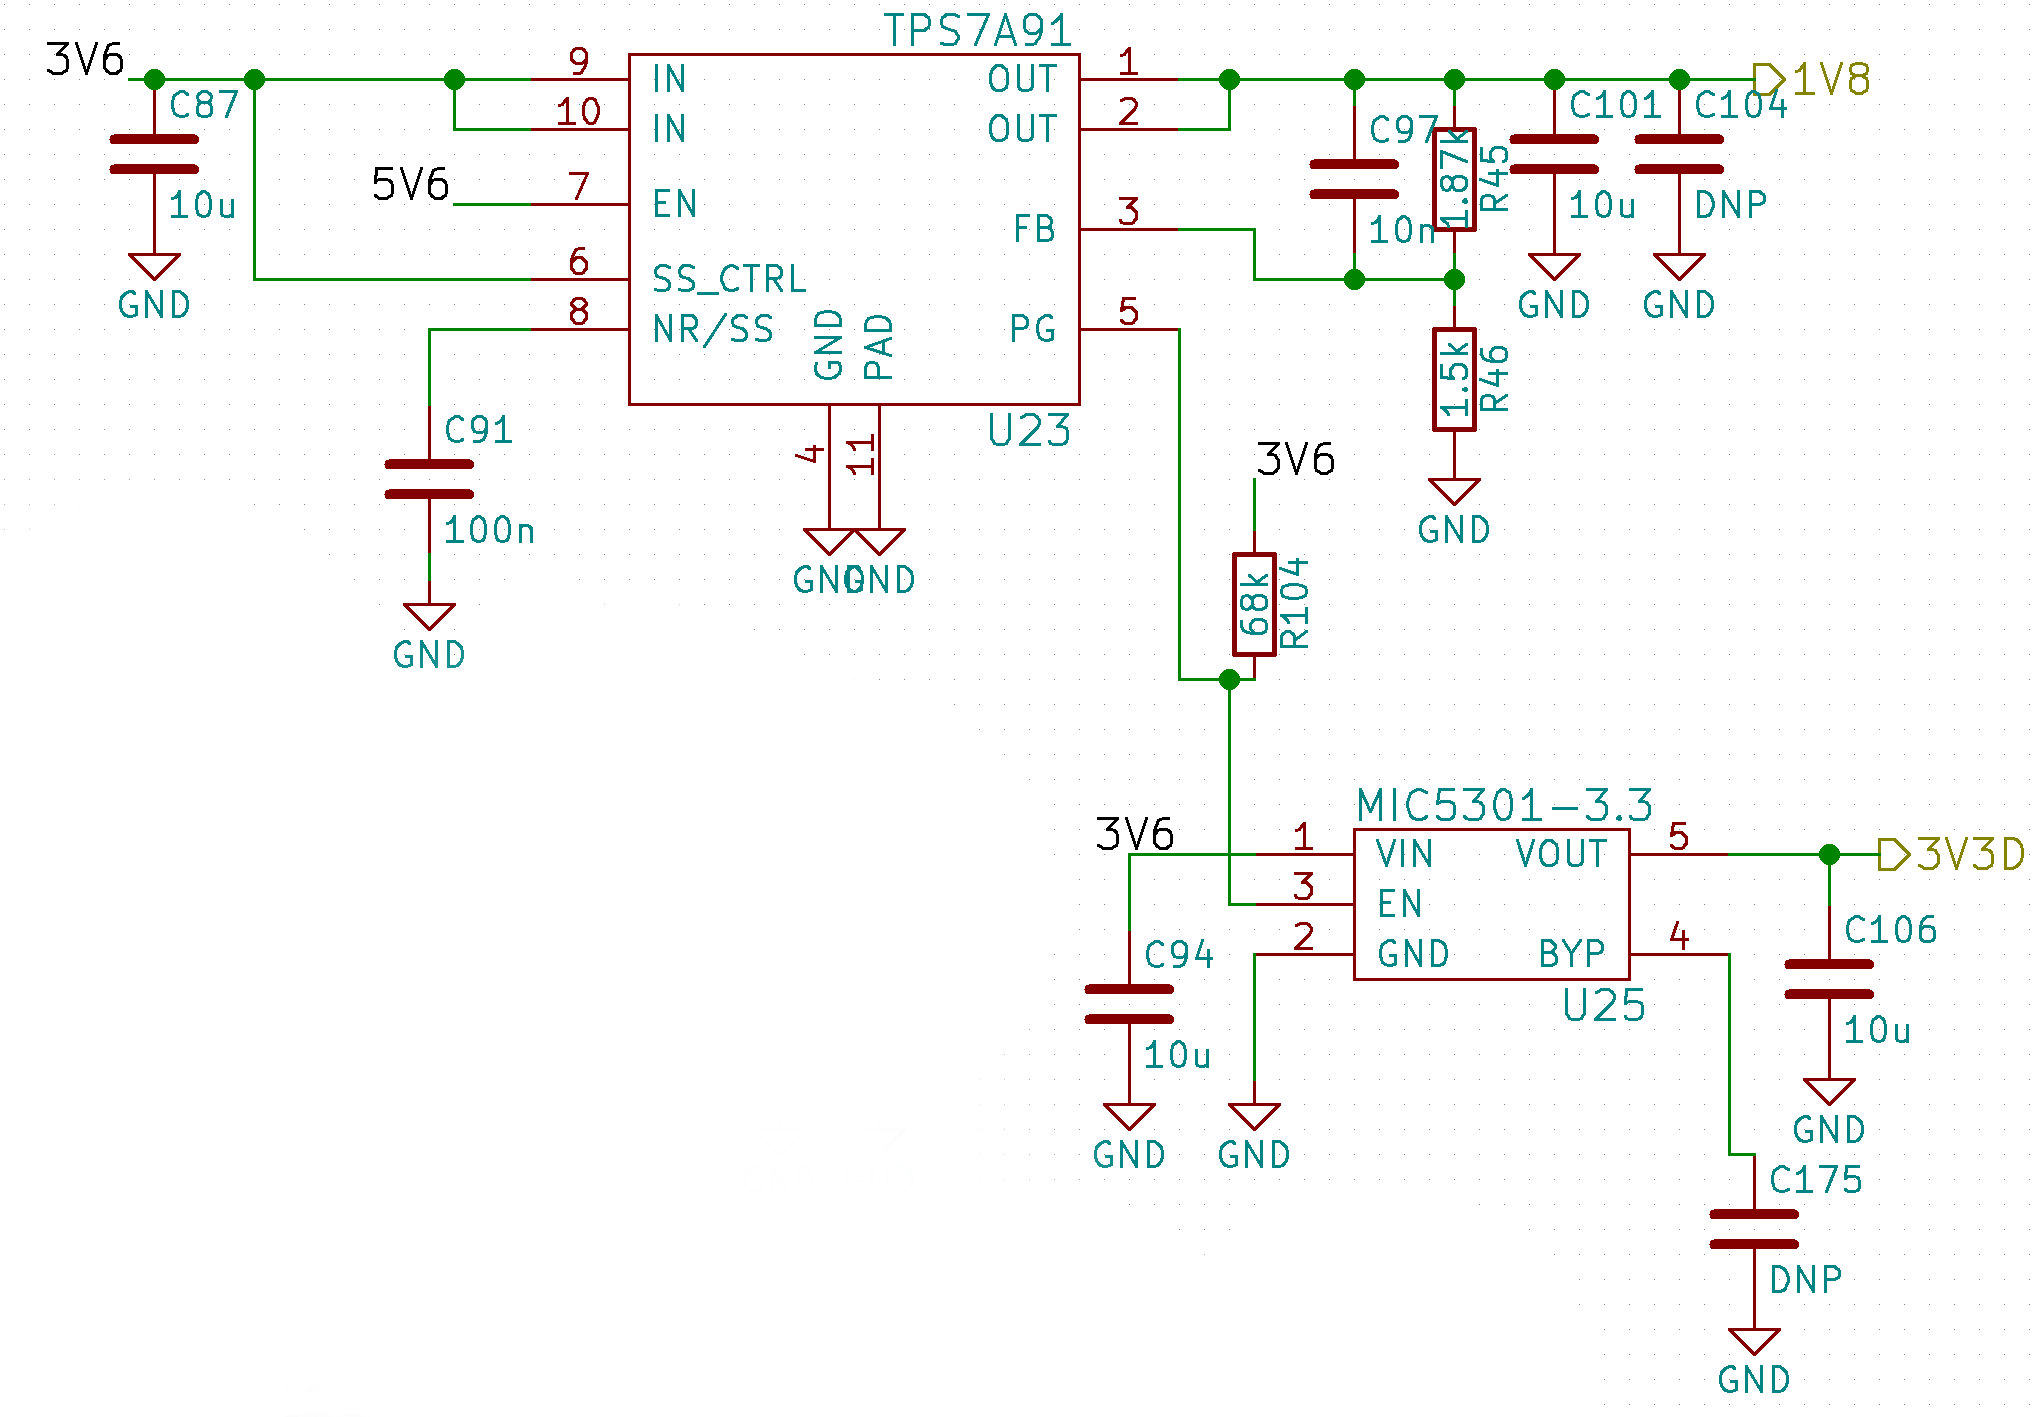
\includegraphics[width=0.9\textwidth]{data/ldo-ldo-connection.png}
  \caption{An ultra LDO regulator whose output feeds into an FPGA input. It uses the PG
    pin from another LDO regulator to alternately enable/disable it.}
  \label{fig:ldo-ldo-connection}
\end{figure}

Another output from a buck converter leads to a 3V output LDO regulator with a dropout voltage of
120mV shown in Figure~\ref{fig:lp5907}. All of the pin connections are evident.

\begin{figure}[h]
  \centering
  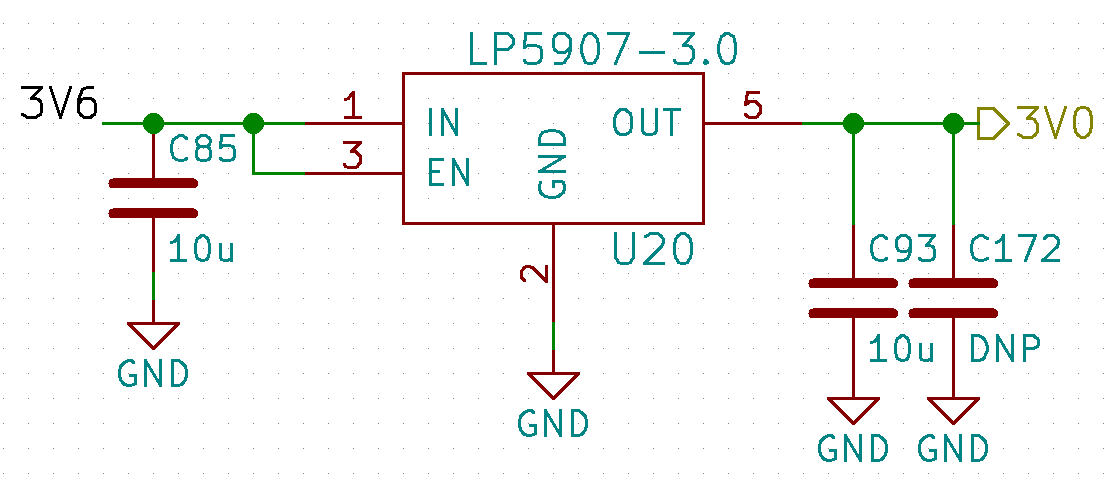
\includegraphics[width=0.75\textwidth]{data/lp5907.png}
  \caption{The LP5907 is a 3V LDO regulator with a dropout voltage of 120mV.}
  \label{fig:lp5907}
\end{figure}

The last component on the power sheet is an
\href{http://www.ti.com/lit/ds/symlink/lp2985.pdf}{LP2985} LDO regulator shown in
Figure~\ref{fig:lp2985}, that takes the 12V input voltage from the barrel jack and outputs
10V. ON/OFF is an active-low shutdown pin, so it is tied to $V_{\text{IN}}$. A 10nF capacitor is
tied to BYPASS to decrease the output noise.

\begin{figure}[h]
  \centering
  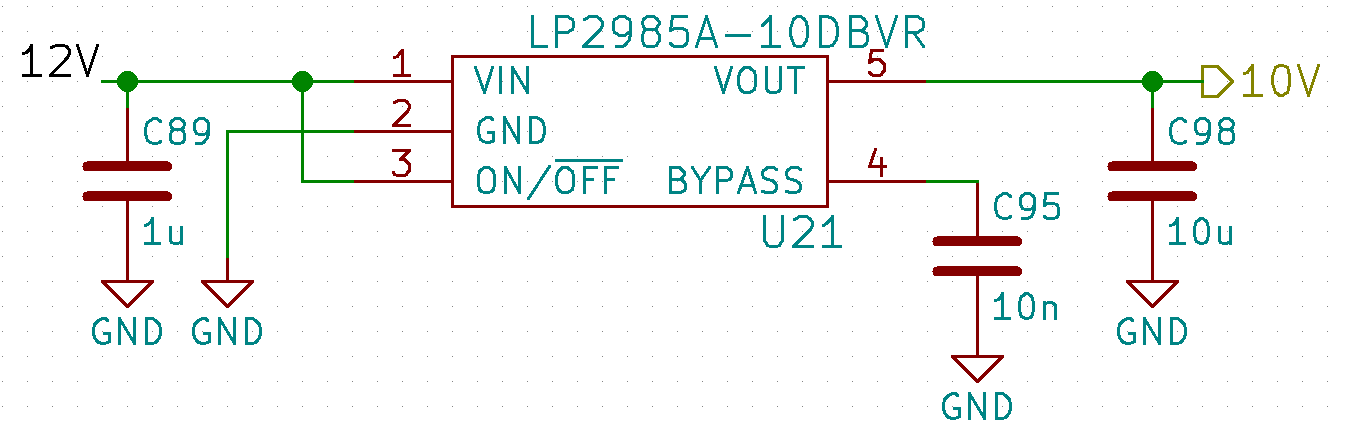
\includegraphics[width=0.9\textwidth]{data/lp2985.png}
  \caption{The LP2985 LDO regulator.}
  \label{fig:lp2985}
\end{figure}

\section{Top Level Schematic}

The top level sheet instantiates the various subcomponents of the design. Additionally, it generates
a 40MHz clock signal that feeds into a clock buffer and is output to various components, as shown in
Figure~\ref{fig:clock-generator}. The LP5907 is a voltage regulator that takes a 3.6V input signal
generated by a buck converter on the power sheet and outputs a 1.8V signal to power the
\href{https://media.digikey.com/pdf/Data\%20Sheets/AVX\%20PDFs/KT2520K40000DAW18TAS_Spec.pdf}{KT2520K}
crystal oscillator which generates a 40MHz clock signal. The coupling capacitor attached in series to
the output of the crystal oscillator will prevent a DC bias from leaving the crystal oscillator. The
Schmitt inverter is used to turn the clipped sine wave output of the crystal oscillator into a
square wave. By connecting the output of the Schmitt inverter back to its input via two resistors
with a bypass capacitor between them, the input sine wave to the trigger becomes centered around
VCC/2, or 1.65V in this case. The capacitor filters out the high frequency signals centers it just at
the DC bias level. The 40MHz square wave feeds into the clock fanout buffer
\href{http://www.onsemi.com/pub/Collateral/NB3N551-D.PDF}{NB3N551} which generates 3 clock outputs
that oscillate at 40 MHz between about 0V and 3V.

\begin{figure}[h]
  \centering
  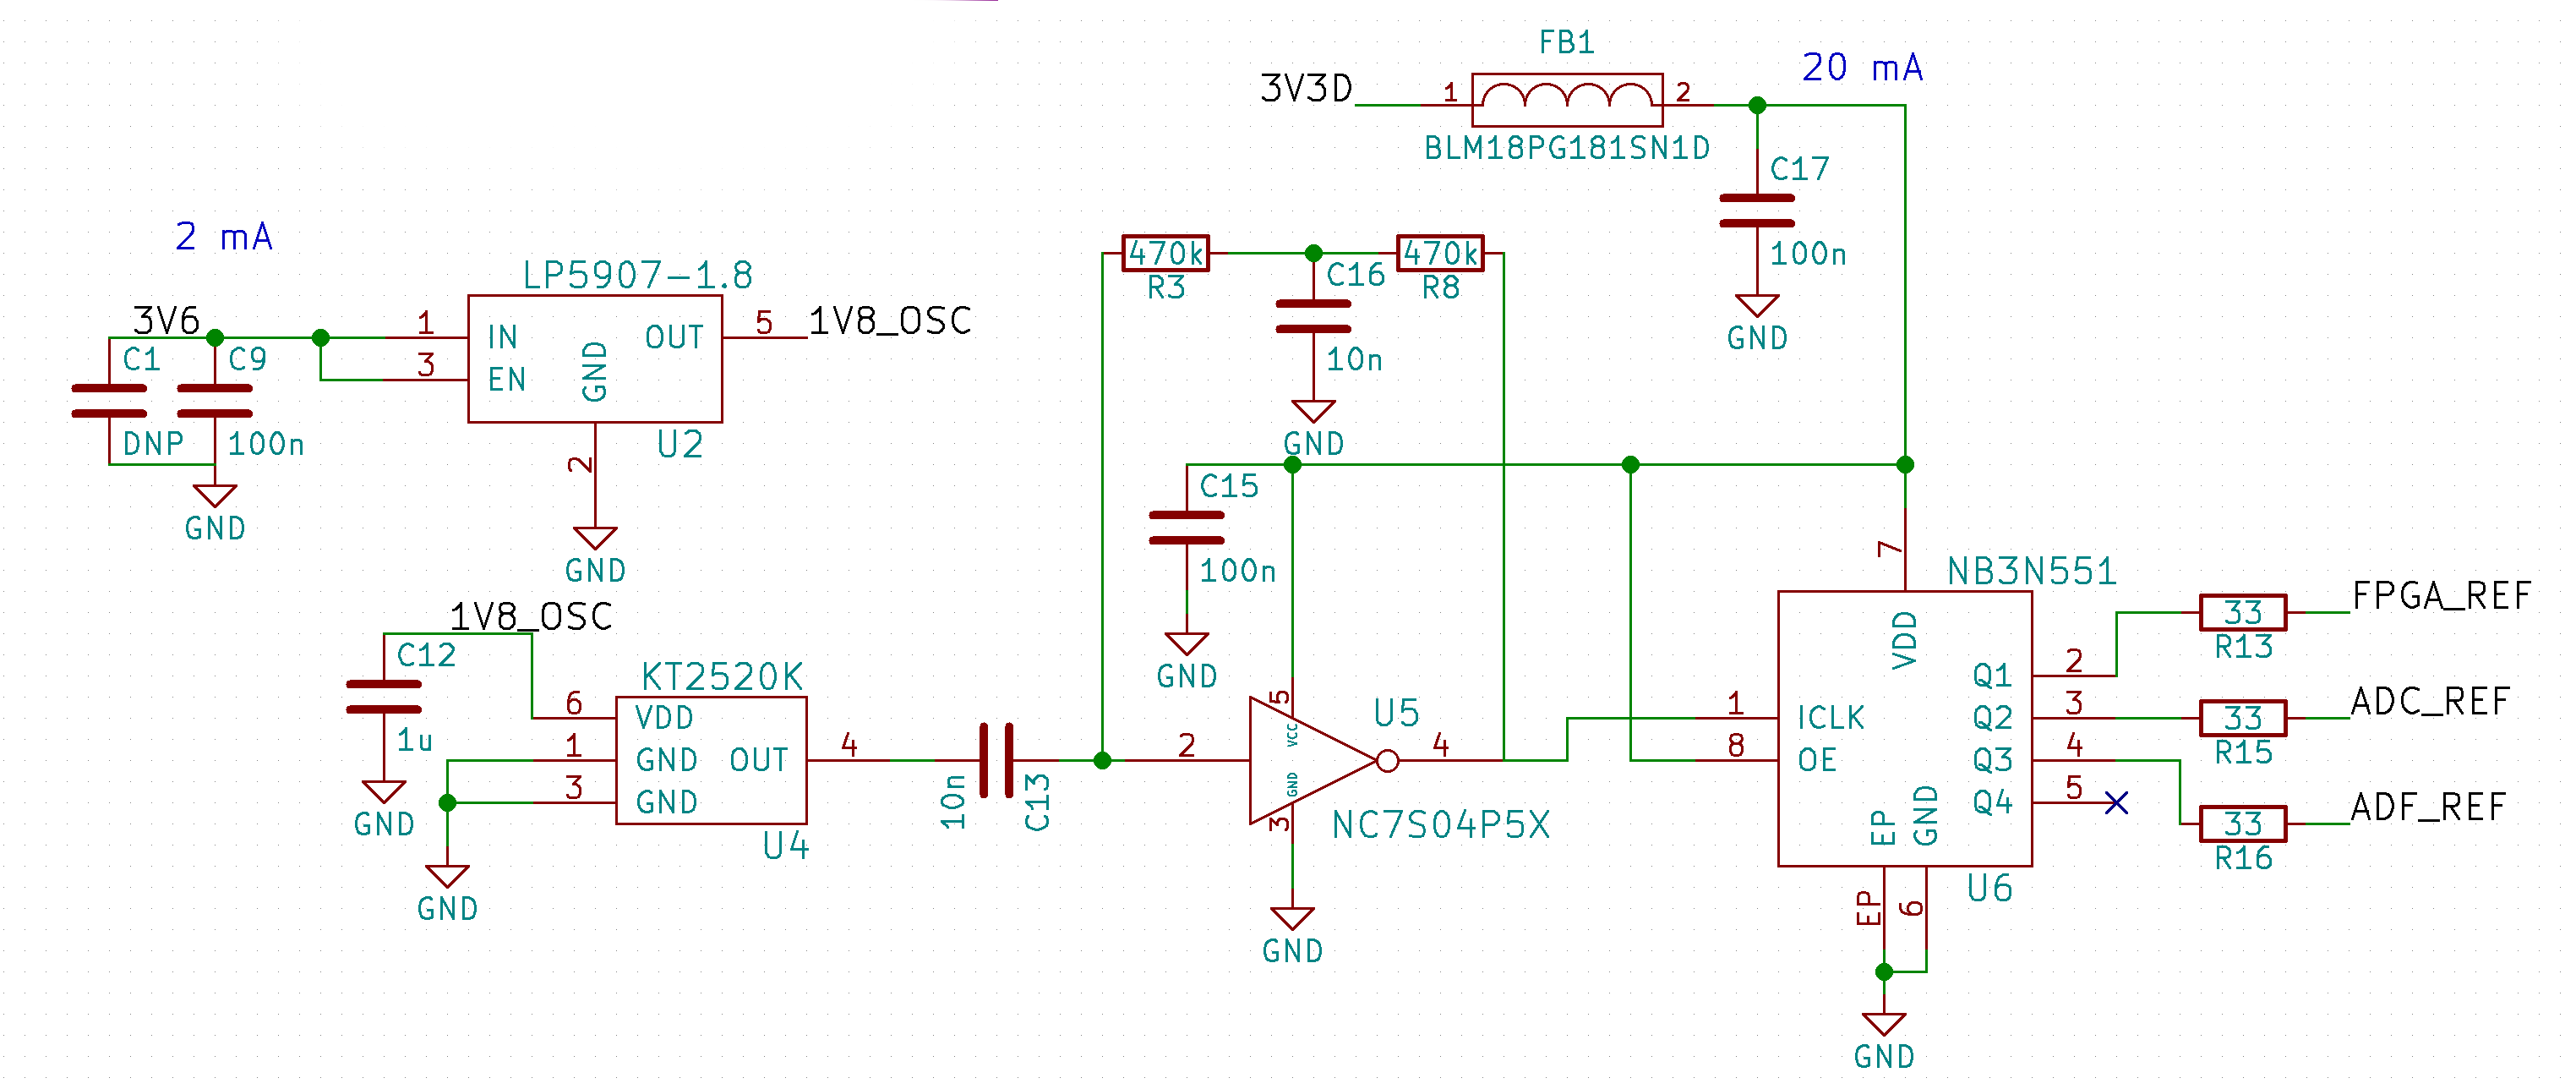
\includegraphics[width=1.0\textwidth]{data/clock-generator.png}
  \caption{A 40MHz clock signal is used to synchronize different components on the board.}
  \label{fig:clock-generator}
\end{figure}

\section{TX}

\includepdf[pages=5, landscape=true, angle=-90]{data/fmcw-schematic.pdf}

\subsection{ADF4158 Frequency Synthesizer}
\label{sec:adf4158-freq-synth}

\subsubsection{Overview}
\label{sec:adf4158-overview}

The \href{http://www.analog.com/media/en/technical-documentation/data-sheets/ADF4158.pdf}{ADF4158}
is a 6.1GHz fractional-n frequency synthesizer. A block diagram describing its functionality is shown in
Figure~\ref{fig:adf4158-block-diagram}.

\begin{figure}[h]
  \centering
  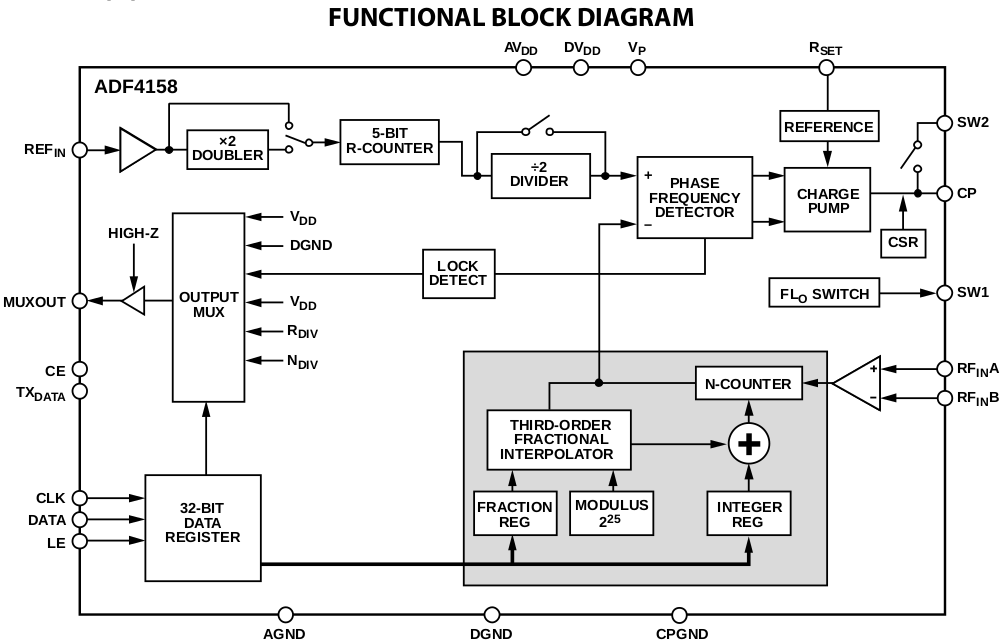
\includegraphics[width=0.75\textwidth]{data/adf4158-block-diagram.png}
  \caption{ADF4158 block diagram.}
  \label{fig:adf4158-block-diagram}
\end{figure}

The ADF4158 relies on an external VCO, described in \cref{sec:hmc431lp4} whose output frequency is
given by Equation~\ref{eq:adf4158-rfout}. The output resolution is
$f_{\text{RES}} = f_{\text{PFD}}/2^{25}$ (see Equation~\ref{eq:adf4158-rfout} and its corresponding
parameter table for an explanation of $f_{\text{PFD}}$). The $2^{25}$ arises from the FRAC value
(set in registers 0 and 1) which is given 25 bits.

\begin{align}
  \text{RF}_{\text{OUT}} &= f_{\text{PFD}} \times \left(\text{INT} +
                           \left(\text{FRAC}/2^{25}\right)\right) \label{eq:adf4158-rfout} \\
  f_{\text{PFD}} &= \text{REF}_{\text{IN}} \times \left[\left(1 + D\right)/\left(R\times \left(1 +
                   T\right)\right) \right] \nonumber
\end{align}

\label{tab:adf4158-rfout-equation-vars}
\begin{tabularx}{\textwidth}{l X>{\raggedright\arraybackslash}X}
  \toprule
  \textbf{Parameter/Variable} & \textbf{Description} \\
  \midrule
  \endhead

  $\text{RF}_{\text{OUT}}$ & The VCO's output frequency. This is the frequency that's amplified for
  transmission. \\
  $f_{\text{PFD}}$ & The input frequency to the PFD post prescaling. In our case this is 20MHz. \\
  INT & The N counter that has a multiplicative effect on the VCO output frequency. \\
  FRAC & FRAC is the numerator of the fractional number added to INT. This is what distinguishes
  fractional-n synthesis from integer-n synthesis. It allows greater precision for the VCO
  output frequency without significantly increasing the prescalers and N counter. \\
  $\text{REF}_{\text{IN}} $ & The reference input frequency, which in our case is a 40MHz clock
  signal from the fanout buffer on the top level of the schematic. \\
  D & The doubler bit, which can be 0 or 1. If set to 1, the $\text{REF}_{\text{IN}}$ frequency is
  doubled before arriving at the R counter. \\
  R & The input prescaler. \\
  T & The divide- by-2 bit, which can be 0 or 1 and divides the frequency by 2 between the R
  prescaler and PFD. \\

  \bottomrule
\end{tabularx}

\subsubsection{Waveform Generation}
\label{sec:adf4158-waveform-generation}

The ADF4158 is capable of producing several different waveforms. The one used in this design is a
sawtooth ramp in frequency as a function of time, shown in Figure~\ref{fig:adf4158-sawtooth-ramp}
. There are 3 different parameters that determine the shape of a ramp:(1)frequency deviation(the
amount the frequency increases at each time step), (2) timeout interval(the amount of time between
each time step) and (3) the number of time steps. This is shown diagrammatically in
Figure~\ref{fig:adf4158-waveform-timing}. The equations governing these parameters are given in
Equation~\ref{eq:adf4158-waveform}. The number of steps is set directly in register 6. In our
configuration $f_{\text{DEV}} = 300\si{kHz}$ and $\text{Timer} = 0.5\si{\mu s}$, which given that
the number of steps is equal to 2000 and the starting frequency is 5.3GHz, the sawtooth will ramp
from 5.3GHz to 5.9GHz in 1ms before repeating.

\begin{align}
  f_{\text{DEV}} &= \left(f_{\text{PFD}}/2^{25}\right) \times \left(\text{DEV}\times
                   2^{\text{DEV\_OFFSET}}\right) \label{eq:adf4158-waveform} \\
  \text{Timer} &= \text{CLK}_1 \times \text{CLK}_2 \times \left(1/f_{\text{PFD}}\right) \nonumber
\end{align}

\label{tab:adf4158-waveform-equation-vars}
\begin{tabularx}{\textwidth}{l X>{\raggedright\arraybackslash}X}
  \toprule
  \textbf{Parameter/Variable} & \textbf{Description} \\
  \midrule
  \endhead

  $f_{\text{DEV}}$ & The frequency deviation for each frequency jump during ramp. \\
  $f_{\text{PFD}}$ & The input frequency to the PFD post prescaling. In our case this is 20MHz. \\
  DEV & A 16-bit value set in register 5. \\
  DEV\_OFFSET & A 4-bit word set in register 5. \\
  Timer & The time between each frequency hop. \\
  CLK\textsubscript{1} & A 12-bit clock divider set in register 2. \\
  CLK\textsubscript{2} & Another 12-bit clock divider set in register 4. \\

  \bottomrule
\end{tabularx}

\begin{figure}[h]
  \centering
  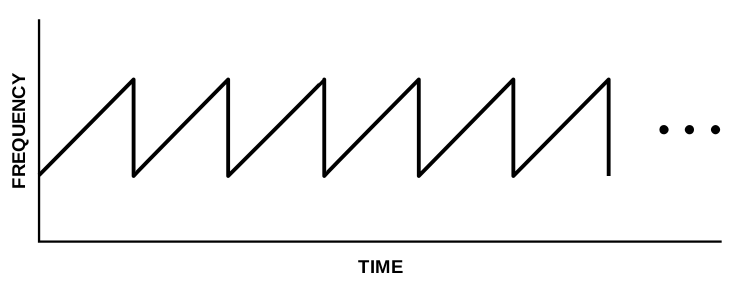
\includegraphics[width=0.5\textwidth]{data/adf4158-sawtooth-ramp.png}
  \caption{Sawtooth ramp.}
  \label{fig:adf4158-sawtooth-ramp}\end{figure}

\begin{figure}[h]
  \centering
  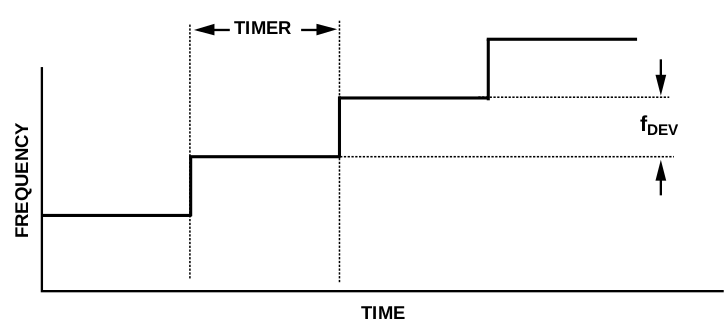
\includegraphics[width=0.5\textwidth]{data/adf4158-waveform-timing.png}
  \caption{Waveform timing.}
  \label{fig:adf4158-waveform-timing}\end{figure}

\subsubsection{Configuration Registers}
\label{sec:adf4158-config-regs}

The ADF4158 contains 8 configuration registers. The configurations are shown in the tables
below. All reserved bits should be set to 0. The control bits are the least significant 3 bits of
each register and are set to the register number for each register (e.g. register 0 is 000 and
register 1 is 001). I've left these out of the tables because their values are obvious.

\label{tab:adf4158-reg-map-0}
\begin{tabularx}{\textwidth}{l l l X>{\raggedright\arraybackslash}X}
  \caption{FRAC/INT REGISTER (R0) MAP} \\
  \toprule
  \textbf{Bits} & \textbf{Mnemonic} & \textbf{Value} & \textbf{DESCRIPTION} \\
  \midrule

  \endhead

  3-14 & FRAC(MSB) & 0 & This sets the 12 most significant bits of FRAC. We leave the fractional
  value at 0. \\
  15-26 & INT & 265 & This is the feedback, or N, counter. \\
  27-30 & MUXOUT Control & 15 & This enables ``readback to muxout'' which allows interrupting
  waveform generation and reading back the frequency at the time of interrupt. The functionality is
  not fully setup on the board(muxout connects to a DNP NMOS) and TX\_DATA, which can trigger the
  interrupt, is set to 0 by the FPGA HDL and left there. \\
  31 & Ramp On & 1 & This bit enables the ramp. \\

  \bottomrule
\end{tabularx}

\label{tab:adf4158-reg-map-1}
\begin{tabularx}{\textwidth}{l l l X>{\raggedright\arraybackslash}X}
  \caption{LSB FRAC REGISTER(R1) MAP} \\
  \toprule
  \textbf{Bits} & \textbf{Mnemonic} & \textbf{Value} & \textbf{DESCRIPTION} \\
  \midrule

  \endhead

  3-14 & Reserved & 0 & All reserved bits set to 0. \\
  15-27 & FRAC(LSB) & 0 & This sets the 13 least significant bits of FRAC. We leave the fractional
  value at 0. \\
  28-31 & Reserved & 0 & All reserved bits set to 0. \\

  \bottomrule
\end{tabularx}

\label{tab:adf4158-reg-map-2}
\begin{tabularx}{\textwidth}{l l l X>{\raggedright\arraybackslash}X}
  \caption{R-DIVIDER REGISTER(R2) MAP} \\
  \toprule
  \textbf{Bits} & \textbf{Mnemonic} & \textbf{Value} & \textbf{DESCRIPTION} \\
  \midrule

  \endhead

  3-14 & CLK\textsubscript{1} Divider & 10 & One of the determinants of the duration of a timestep in
  waveform generation. See \cref{sec:adf4158-waveform-generation} for more details. \\
  15-19 & R-Counter & 1 & This 5-bit segment is used to divide the frequency of the reference signal
  before it enters the PFD. We leave it at 1 and thus do not use it to divide the frequency. \\
  20 & Reference Doubler & 0 & We leave this at 0 and thus do not use the doubler to double the
  reference signal frequency before input to the PFD. The maximum input frequency for the PFD is
  30MHz and so doubling our 20MHz signal (we used the divider to divide the 40MHz signal by 2) would
  violate this condition. \\
  21 & RDIV2 & 1 & Inserts a divide-by-2 toggle flip-flop between the R-counter and PFD. This
  provides a 50\% duty cycle that allows cycle slip reduction to be used which improves lock times. \\
  22 & Prescaler & 1 & The prescaler limits the INT value and through that the maximum frequency to
  3GHz. Since we have an INT value of 265 and our maximum frequency is almost double 3GHz we set
  this to 1. \\
  23 & Reserved & 0 & All reserved bits set to 0. \\
  24-27 & Charge Pump Current Setting & 0 & Sets the current to the minimum value which is 0.31mA
  and is the level necessary to use cycle slip reduction which we are. \\
  28 & CSR Enable & 1 & Enables cycle slip reduction which provides better lock times. \\
  29-31 & Reserved & 0 & All reserved bits are set to 0. \\

  \bottomrule
\end{tabularx}

\label{tab:adf4158-reg-map-3}
\begin{tabularx}{\textwidth}{l l l X>{\raggedright\arraybackslash}X}
  \caption{FUNCTION REGISTER(R3) MAP} \\
  \toprule
  \textbf{Bits} & \textbf{Mnemonic} & \textbf{Value} & \textbf{DESCRIPTION} \\
  \midrule

  \endhead

  3 & Counter Reset & 0 & When this is set to 1, the synthesizer counters are held in reset. For
  normal operation we set this to 0. \\
  4 & Charge Pump Three-State & 0 & Holds the charge pump in three-state mode if set to 1. For
  normal operation it must be set to 0. \\
  5 & Power-Down & 0 & Setting this to 1 powers down the device. Setting it to 0 allows normal
  operation. \\
  6 & PD Polarity & 1 & Set to 1 for positive VCO characteristics. Set to 0 for negative VCO
  characteristics. Since our VCO outputs a positive voltage signal we set this to 1. \\
  7 & LDP & 0 & Sets the minimum number of PFD cycles before a lock detect can be set. \\
  8 & FSK Enable & 0 & Disables FSK modulation. \\
  9 & PSK Enable & 0 & Disables PSK modulation. \\
  10-11 & Ramp Mode & 0 & Sets the waveform as a continuous sawtooth. \\
  12-13 & Reserved & 0 & All reserve bits are set to 0. \\
  14 & SD Reset & 0 & Setting this to 0 resets the $\Sigma-\Delta$ modulator on each write to
  register 0, which is the recommended operation. Setting this to 1 disables resetting the
  modulator. \\
  15 & N SEL & 0 & When set to 1, this creates an additional delay in setting INT and FRAC which can
  prevent the PLL overshooting. Since we set INT once and do not update it, this is not necessary
  and we leave it as 0. \\
  16-31 & Reserved & 0 & All reserve bits are set to 0. \\

  \bottomrule
\end{tabularx}

\label{tab:adf4158-reg-map-4}
\begin{tabularx}{\textwidth}{l l l X>{\raggedright\arraybackslash}X}
  \caption{TEST REGISTER(R4) MAP} \\
  \toprule
  \textbf{Bits} & \textbf{Mnemonic} & \textbf{Value} & \textbf{DESCRIPTION} \\
  \midrule

  \endhead

  3-6 & Reserved & 0 & All reserved bits are set to 0. \\
  7-18 & CLK\textsubscript{2} Divider & 1 & This is used to set the timeout interval in ramp
  generation. See \cref{sec:adf4158-waveform-generation}for more information. \\
  19-20 & CLK DIV Mode & 3 & This enables ramp divider mode, which specifies that
  CLK\textsubscript{1} and CLK\textsubscript{2} are used for ramp generation. \\
  21-22 & Readback to MUXOUT & 3 & Confusingly, this has been set to 3, which corresponds to neither
  of the supported values. Since we don't actually use the MUXOUT, this seems to be fine. If, at
  some point in the future, we do use the MUXOUT we will probably need to fix this. \\
  23-24 & Negative Bleed Current & 0 & This setting can help improve performance in the dead
  zone. We've disabled it. Note that this setting and readback to MUXOUT cannot simultaneously be
  enabled. To understand this setting better refer to
  \href{http://www.analog.com/media/en/technical-documentation/application-notes/AN-1154.pdf?doc=ADF4158.pdf}{AN-1154
    Application Note}. \\
  25 & Reserved & 0 & All reserved bits are set to 0. \\
  26-30 & $\Sigma-\Delta$ modulator mode & 0 & 0 enables this during normal operation. We can set it
  to 14 when FRAC=0. Even though we've set FRAC to 0, we have left this as 0 which seems strange. It
  shouldn't cause anything to malfunction, but may cause the ADF4158 to draw more power. We should
  experiment with setting this to 14 when using the actual board. \\
  31 & LE SEL & 0 & LE is the load enable pin which we use to load data onto the ADF4158's internal
  registers. Setting this to 0 enables the default operation of using the pin to set LE. Setting it
  to 1 would synchronize it with the reference signal. \\

  \bottomrule
\end{tabularx}

\label{tab:adf4158-reg-map-5}
\begin{tabularx}{\textwidth}{l l l X>{\raggedright\arraybackslash}X}
  \caption{DEVIATION REGISTER (R5) MAP} \\
  \toprule
  \textbf{Bits} & \textbf{Mnemonic} & \textbf{Value} & \textbf{DESCRIPTION} \\
  \midrule

  \endhead

  3-18 & DEVIATION WORD & 31457 & This is used to set the size of successive frequency jumps during
  ramp. See \cref{sec:adf4158-waveform-generation} for more information. \\
  19-22 & DEVIATION OFFSET & 4 & This is also used to set the size of successive frequency jumps during
  ramp. See \cref{sec:adf4158-waveform-generation} for more information. \\

  \bottomrule
\end{tabularx}


\label{tab:adf4158-reg-map-6}
\begin{tabularx}{\textwidth}{l l l X>{\raggedright\arraybackslash}X}
  \caption{STEP REGISTER (R6) MAP} \\
  \toprule
  \textbf{Bits} & \textbf{Mnemonic} & \textbf{Value} & \textbf{DESCRIPTION} \\
  \midrule

  \endhead

  3-22 & STEP WORD & 2000 & This determines the number of steps in a ramp. To understand this see
  \cref{sec:adf4158-waveform-generation} on waveform generation. \\

  \bottomrule
\end{tabularx}


\label{tab:adf4158-reg-map-7}
\begin{tabularx}{\textwidth}{l l l X>{\raggedright\arraybackslash}X}
  \caption{DELAY REGISTER (R7) MAP} \\
  \toprule
  \textbf{Bits} & \textbf{Mnemonic} & \textbf{Value} & \textbf{DESCRIPTION} \\
  \midrule

  \endhead

  19-31 & Reserved & 0 All reserve bits are set to 0. \\

  \bottomrule
\end{tabularx}


\paragraph{FIXME} I need to finish describing this component along with all other component on this
sheet.

\label{tab:adf4158-pins}
\begin{tabularx}{\textwidth}{l l X>{\raggedright\arraybackslash}X}
  \caption{All ADF4158 pin connections.} \\
  \toprule
  \textbf{PIN} & \textbf{Mnemonic} & \textbf{DESCRIPTION} \\
  \midrule

  \endhead

  1 & CPGND & \\
  2, 3 & AGND &\\
  4 & RF\textsubscript{IN} B & \\
  5 & RF\textsubscript{IN} A & \\
  6, 7, 8 & AV\textsubscript{DD} & \\
  9 & REF\textsubscript{IN} & \\
  10 & DGND & \\
  11 & SDGND & \\
  12 & TX\textsubscript{DATA} & \\
  13 & CE & \\
  14 & CLK & \\
  15 & DATA & \\
  16 & LE & \\
  17 & MUXOUT & \\
  18 & SDV\textsubscript{DD} & \\
  19 & DV\textsubscript{DD} & \\
  20, 21 & SW1, SW2 & \\
  22 & V\textsubscript{P} & \\
  23 & R\textsubscript{SET} & \\
  24 & CP & \\
  25 & EPAD &\\

  \bottomrule
\end{tabularx}

\subsection{HMC431LP4RF VCO}

\label{sec:hmc431lp4rf}
The
\href{http://www.analog.com/media/en/technical_documentation/data_sheets/hmc431.pdf}{HMC431LP4RF} is a radio-frequency VCO.

The MGA-25203 power amplifier is now obsolete and there are no alternatives with an identical
interface. Therefore the design will need to be modified. The alternative I will use is the
\href{http://www.skyworksinc.com/uploads/documents/202425A.pdf}{SE2567L} which seems to be very
similar. There are a few small differences in addition to the pin differences: the original device
has a power output of 23dBm in contrast to the new device which has a power output of 21.5dBm when
VCC0,1=3.3V and VCC2,3=4.5V. I believe this is close enough to not create any issues, especially as
they are both quoted as having 30dB gain and are IEEE 802.11-compliant. Additionally, the original
device has a load current about twice that of the new device. Since the output powers are relatively
similar (and the overview of original design describes a 20dB gain), I don't believe this should be
an issue. The original chip contains BCTRL, BSW, and BSPLY that differ from the new chip. BCTRL
regulates the device current and is kept at a constant 2.8V. There is no analogous pin on the new
chip. BSW is an enable pin that turns on the device when set to 1.8V. When it is set to 0V, the
device is turned off. The original design uses a MOSFET transistor with a drain of 1.8V, source at
GND and gate controlled by the FPGA (when the gate is activated the BSW pin gets a voltage of 0V and
is disabled). The new chip contains an analogous pin, EN, which enables the power amplifier at the
input voltage level 3.3V and disables it at GND. So, to get analogous functionality, we should
connect the MOSFET drain to 3.3V instead of 1.8. Everything else should stay the same. BSPLY simply
received the input voltage of 3.3V. In the new chip, the pins that are different from the original
chip (and not already discussed) are VCC0-3 and DET. DET is a pin that outputs a voltage indicating
the power output. We should connect this to a DNP capacitor to GND to be able to detect the output
power of the amplifier with an ammeter. VCC0-1 should be connected to the 3.3V power supply. In
order to get the additional power output, we should connect VCC2-3 to a 4.5V power supply instead of
3.3V. Unfortunately, it isn't possible to simply repurpose the voltage divider to the BCTRL pin for
this since I do not know the internal impedance of the power amplifier IC and in general voltage
dividers are bad for supplying power. Additionally, the simple LP5907 voltage divider may not work
since it is only rated to 250mA of current, which doesn't leave much room above the 220mA expected
by the SE2567L. It seems to make the most sense to use the
\href{http://www.ti.com/lit/ds/symlink/tps7a91.pdf}{TPS7A91} which is rated to 1A. It has the
downside of requiring additional hardware which will need to be adjusted in the PCB accordingly. To
get the correct output voltage of 4.5V, we need to use Equation~\ref{eq:linear-reg-vout}. Since the
datasheet doesn't specify the resistors for a 4.5V output voltage this takes a bit of art to finding
the correct resistors. Ideally, we want resistors with a higher-value so that less power is
dissipated, and are commonly used to reduce cost and make them easier to replace if
necessary. Lastly, I'd like to keep the values in the ballpark of those specified in the datasheet
in case there are any other reasons I'm not thinking of. The values $R_2 = 1.47\si{k\Omega}$ and
$R_1 = 6.8\si{k\Omega}$ should work well. The modified schematic for this is shown in
Figure~\ref{fig:se2567l}.

\begin{figure}[h]
  \centering
  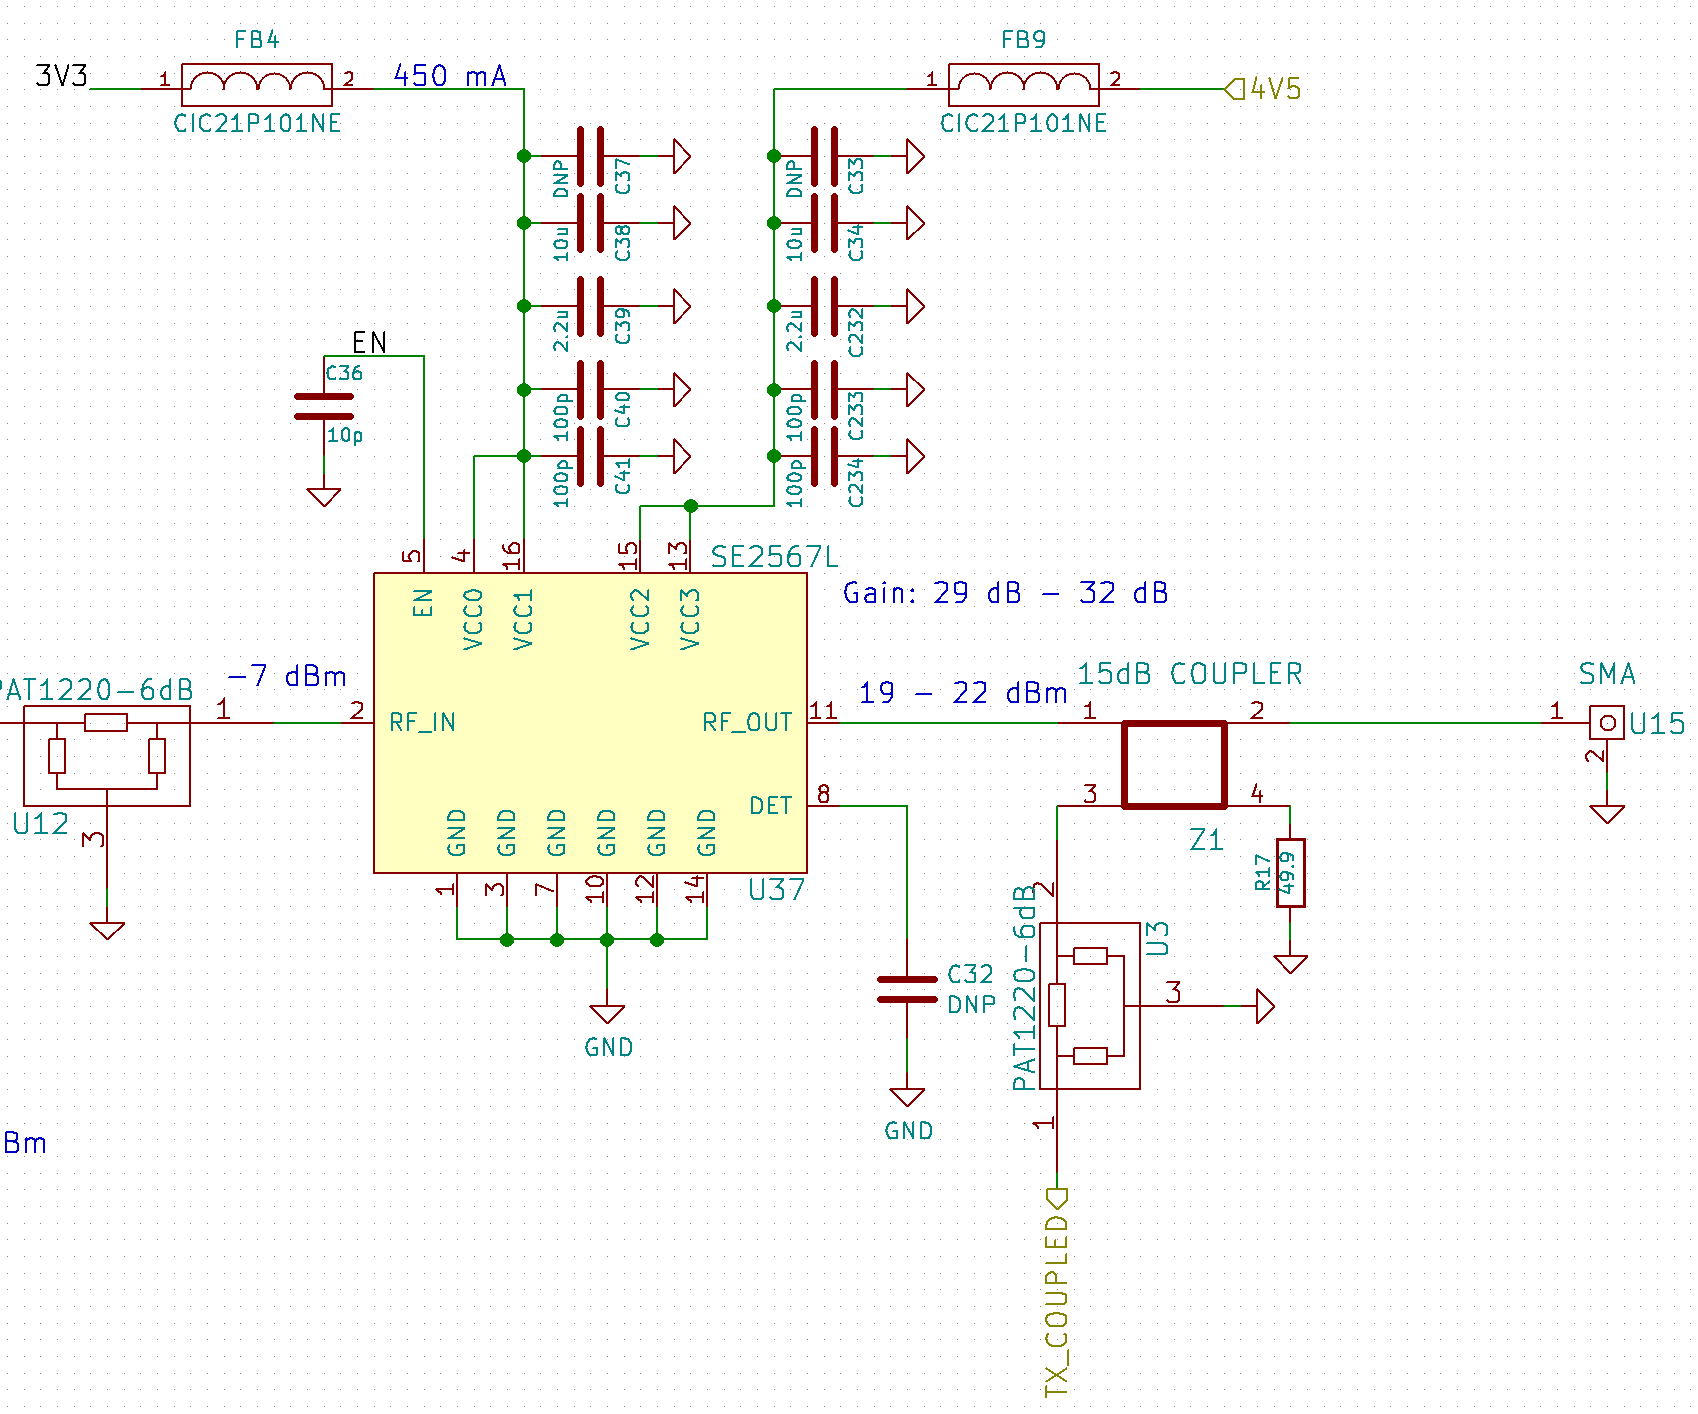
\includegraphics[width=\textwidth]{data/se2567l.png}
  \caption{The SE2567L power amplifier. This has been modified from the original design due to the
    old power amplifier having been discontinued.}
  \label{fig:se2567l}
\end{figure}

\section{USB}

In order to configure the FPGA we load the configuration bit stream onto the board using a US cable
and USB micro receptor on the PCB. The signal is then passed along to
an \href{http://www.ftdichip.com/Support/Documents/DataSheets/ICs/DS_FT2232H.pdf}{FT2232H} IC
that translates the USB signal into JTAG data which it sends to the FPGA using the TCK, TDI, TDO and
TMS pins. The schematic for this is shown in Figure~\ref{fig:usb-ft2232}. The FT2232H IC
requires several power inputs: 3 VCORE input pins that require a 1.8V input voltage (this comes from
VREGOUT, which is a pin that outputs a 1.8V signal from an internal voltage regulator), 1 3.3V VREGIN
input (which serves as the input pin to drive the 1.8V regulated output), 4 3.3V VCCIO input pins,
and 23.3V inputs (VPLL and VPHY) that are filtered with an LC filter.

\paragraph{FIXME} I'm a bit confused as to the operation of the LC filter. It is implemented as a
ferrite bead with two parallel capacitors in parallel with the load. This feeds in from an LDO
regulator that in turn received its input from a buck converter operating at roughly 700kHz. The
frequency at which the ferrite bead is in its resistive state is around 100MHz, well above the
switching regulator noise. Maybe the filter is meant to filter out noise other than that from the
buck converter. For instance, it is possible that the LDO regulator used after the buck converter
(which has a PSRR near 0 around 500kHz and above) is sufficient for filtering the switching
noise. The Art of Electronics states that ferrite beads should be placed at different points
throughout the design to raise impedance at high frequencies. It is possible that this is the
functionality provided by these ferrite beads.  OSCI and OSCO are the oscillator input and output,
respectively. These must be connected to a 12MHz oscillator with a frequency tolerance less than
30ppm (ours is 10ppm). REF is a current reference that must be connected to a 12k$\Omega$ resistor to
ground. DM and DP are the USB data signal minus and plus lines, respectively. TEST should be
connected to ground. RESET\# (the \# indicates an active low pin) is connected to a pull-up resistor
to 3.3V so the reset is deasserted whenever the input voltage is at a sufficiently high and stable
level. PWREN\# is an output that is 0 during normal operation. We don't need it here so we leave it
floating. SUSPEND\# is similar to PWREN\#; it is low when the USB is in suspend mode. This is used as
an input to the FPGA. BDBUS0-3 are used for the JTAG interface to configure the FPGA. In order, they
are TCK, TDI, TDO and TMS.

\paragraph{FIXME} The FT2232H device also communicates with the FPGA using a synchronous FIFO
interface as described
\href{http://www.ftdichip.com/Support/Documents/AppNotes/AN_130_FT2232H_Used_In_FT245\%20Synchronous\%20FIFO\%20Mode.pdf}{here}. This
seems to be the way that data is sent between the FPGA and the host computer although I'm not
clear how this works. In any event, it uses the ADBUS0-7 and ACBUS0-7 pins. The ADBUS pins
are bidirectional pins that serve as the FPGA side translation of the USB data. In other words,
they should allow the FPGA to read USB data from a host computer and send data back to that host
computer through a USB cable. The ACBUS lines seem to be used to signal reads/writes/etc. It also
seems to require the external EEPROM storage IC,
\href{http://ww1.microchip.com/downloads/en/DeviceDoc/20001749K.pdf}{93LC46B} although I'm not sure
why this interface requires additional, external memory.

\begin{figure}[h]
  \centering
  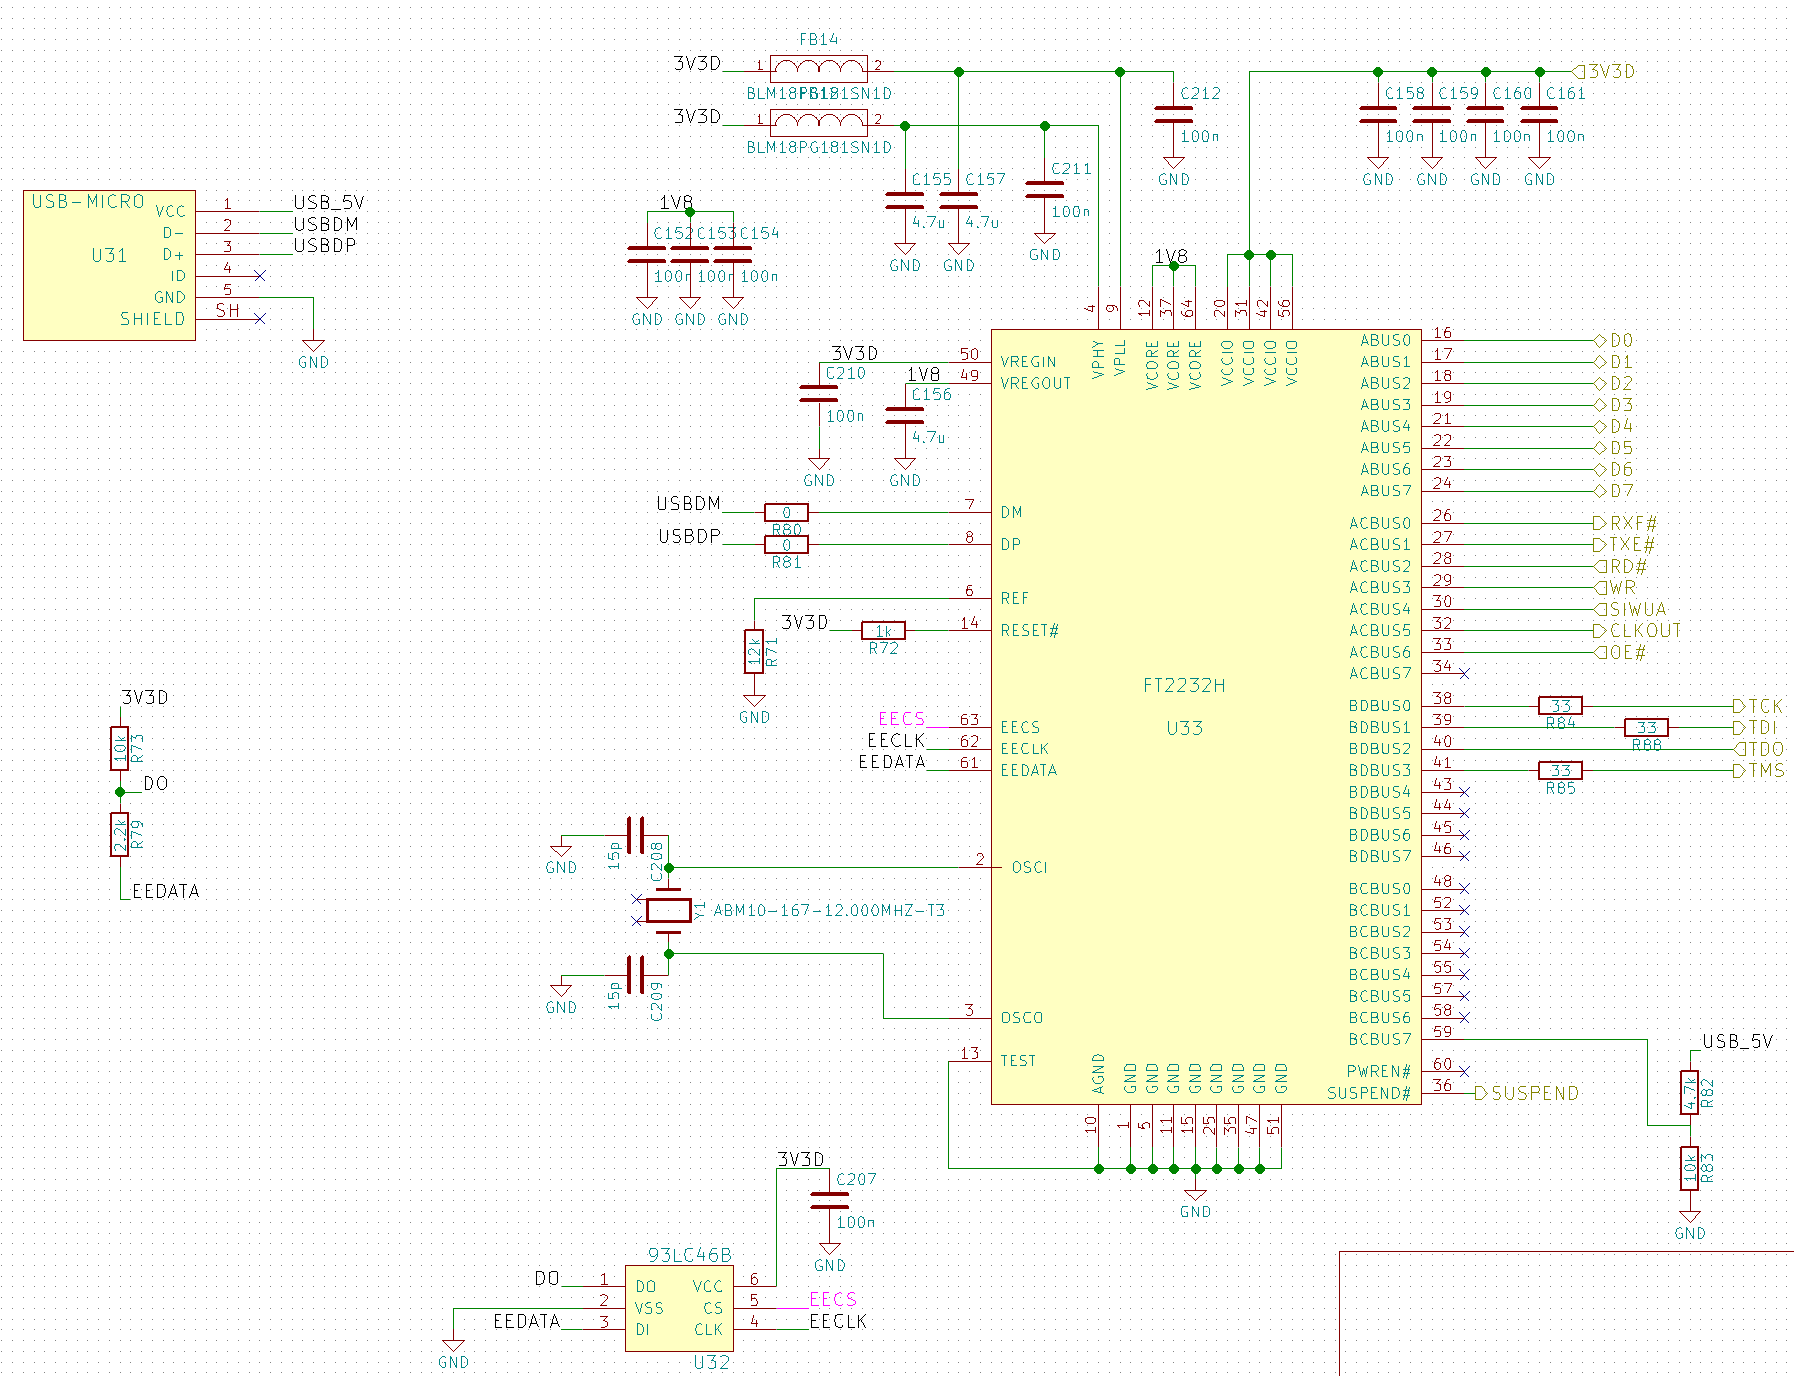
\includegraphics[width=\textwidth]{data/usb-ft2232.png}
  \caption{The configuration bit stream is loaded onto the FPGA using a USB-JTAG interface.}
  \label{fig:usb_ft2232}
\end{figure}

\section{FPGA}
There are several different documents for the
\href{https://www.xilinx.com/products/silicon-devices/fpga/artix-7.html?resultsTablePreSelect=documenttype:Data\%20Sheets#documentation}{Artix-7
  FPGA family}, which is used for this radar. There is a
\href{https://www.xilinx.com/support/documentation/user_guides/ug475_7Series_Pkg_Pinout.pdf}{package-pinout
  document} that, as its name suggests, contains information about the various package options
available and the associated pin definitions. There is an
\href{https://www.xilinx.com/support/documentation/data_sheets/ds180_7Series_Overview.pdf}{overview
  sheet} that contains very general information about the FPGA. There is a
\href{https://www.xilinx.com/support/documentation/user_guides/ug483_7Series_PCB.pdf}{PCB design
  guide} document that contains recommendations for soldering the FPGA on a PCB. There is a
\href{https://www.xilinx.com/support/documentation/user_guides/ug480_7Series_XADC.pdf}{XADC
  document} which describes the mixed-signal functionality of the FPGA. Finally, there is a
\href{https://www.xilinx.com/support/documentation/user_guides/ug470_7Series_Config.pdf}{configuration
  guide} that describes the different ways to configure the FPGA with a bitstream. The FPGA pins
follow a logical syntax: they can be of the form IO\_LXXY\_ZZZ\_\#, IO\_XX\_ZZZ\_\#, or a specific
name. If they have a specific name, they have a dedicated function described starting on page 26 of
the package-pinout document. If they have the general form IO\_LXXY\_ZZZ\_\# or IO\_XX\_ZZZ\_\#,
they can be used for several different dedicated functions, or as general purpose IO pins. L
indicates that the pin can be used as a differential pair (differential signaling), where Y=P or N
depending on whether the pin is the positive or negative side of the differential pair. XX gives a
unique number identifier that can be used to associate the two different pins forming a differential
pair. ZZZ represents one or more functions that the pin can be used for in addition to general
purpose IO. \# indicates the bank number, which separate the pins into one of several different
regions. The package used in this design is FTG256C, which contains banks 0, 14, 15, 34 and 35. Bank
0 contains the dedicated configuration pins. Each bank has 4 pairs of clock capable inputs for
differential or single ended clocks (there are no global clock pins). The bypass capacitor
recommendations are outlined in the PCB design guide. As with any other bypass capacitor design,
place the small caps as close to the pins they connect to as possible. The larger caps should also
be as close as possible, but give priority to the small caps.  The FPGA loads its configuration from
an SPI flash memory device,
\href{http://www.winbond.com/resource-files/w25q32jv\%20revg\%2003272018\%20plus.pdf}{W25Q32JV} The
CCLK\_0 pin is exported from the FPGA to the flash device to drive its operation and coordinates
writes and reads to and from the device. DO is used by the FPGA to perform SPI reads from the flash
memory device. It is connected to J14 of the FPGA. DI is connected to J13 of the FPGA and is used by
the FPGA to send data to the flash memory device. CS is active low and is used by the FPGA to signal
data transmission is about to occur. It is connected to L12 on the FPGA. WP (write protect) and HOLD
are both active low pins and are used to prevent the status configuration registers from being
written to and can pause the device when multiple devices share the same SPI signal, respectively
They are unused and thus connected to the 3.3V power supply. The device is powered with 3.3V (it
supports a range of 2.7V to 3.6V). Table~\ref{tab:fpga-pins} contains a list of all FPGA pins and
their connections.

\label{tab:fpga-pins}
\begin{tabularx}{\textwidth}{c X>{\raggedright\arraybackslash}X}
  \caption{All FPGA pin connections in alphabetical order.} \\
  \toprule
  \textbf{PIN} & \textbf{DESCRIPTION} \\
  \midrule
  \endhead

  A01 & GND. \\
  A02 & Connected to an external 1x1 pin header that is currently unused by FPGA logic. \\
  A03 & Connected to external 2x4 pin header that is currently unused by FPGA logic. \\
  A04 & Connected to same pin header as A03. Also unused. \\
  A05 & Same. \\
  A06 & One of the voltage supplies for bank 35. It uses 3.3V as with all the other voltage supplies
  to the main banks of the FPGA. \\
  A07 & Connected to same pin header as A03. Unused. \\
  A08 & A different 2x4 pin header. Unused. \\
  A09 & Connected to the same pin header as A08. Unused. \\
  A10 & Floating. \\
  A11 & GND. \\
  A12 & Connected as an output to the FT2232H USB-JTAG converter. Pulling this low allows the
  FT2232H device to output data to the FPGA through the ADBUS pins. Driving it high sets the ADBUS
  pins as inputs. Remember, the ADBUS pins serve as the bidirectional translation between JTAG data
  and USB data. \\
  A13 & SIWU (channel A). This pin is output to the FT2232H device and can be used to optimize USB
  data transfers (more info in the FT2232H datasheet). It is not currently used by the FPGA
  logic. \\
  A14 & Write output pin to the FT2232H device. When this is driven low, the FPGA writes data to the
  FT2232H. When it's driven high, the FPGA can perform a read from the FT2232H. \\
  A15 & Inputs a 60MHz clock signal that originated at the FT2232H. This clock is used to
  synchronize all data transfers between the FPGA and the FT2232H. \\
  A16 & A 3.3V input to bank 15. \\

  \midrule

  B01 & ADC\_SHDN1. One of two ADC\_SHDN outputs that, together with OEA (B02), controls the
  shutdown mode selection of the ADC. It is used by the digital FPGA logic. When both SHDN and OE
  are grounded, the ADC performs normally. When they are both pulled high, the ADC goes into sleep
  mode. There are two other states but they are not used by the FPGA logic. \\
  B02 & ADC\_OE1. See pin B01. This is used for channel A. \\
  B03 & 3.3V input for bank 35. \\
  B04 & Floating. \\
  B05 & Connected to the same 2x4 pin header as A03. Unused. \\
  B06 & Floating. \\
  B07 & Connected to the same 2x4 pin header as A03. Unused. \\
  B08 & GND. \\
  B09 & Connected to the same pin header as A08. Unused. \\
  B10 & Connected to the same pin header as A08. Unused. \\
  B11 & Floating. \\
  B12 & Floating. \\
  B13 & 3.3V input for bank 15. \\
  B14 & RD\#. A read active-low output pin to the FT2232H device. When this is driven low, the FPGA
  reads data from the FT2232H. \\
  B15 & TXE\#. An active-low input from the FT2232H. FT2232H drives this pin low to signal sending
  data to the FPGA (i.e. a read for the FPGA). \\
  B16 & RXF\#. An active-low input from the FT2232H. FT2232H drives this pin low to signal that it
  should read data. To the FPGA, this signals that it should write data. \\

  \midrule

  C01 & Floating. \\
  C02 & OF1. An input from the ADC. It is pulled high when an overflow or underflow occurs at
  channel A. It is currently unused by the FPGA logic. \\
  C03 & Floating. \\
  C04 & Floating. \\
  C05 & GND. \\
  C06 & Floating. \\
  C07 & Floating. \\
  C08 & Floating. \\
  C09 & Floating. \\
  C10 & 3.3V input to bank 15. \\
  C11 & Connected to the same pin header as A08. Unused. \\
  C12 & Connected to the same pin header as A08. Unused. \\
  C13 & Floating. \\
  C14 & Floating. \\
  C15 & GND. \\
  C16 & FT\_SUSPEND. An active-low input to the FPGA. FT223H drives this low when the USB is in
  suspend mode. It is currently unused by the FPGA logic. \\

  \midrule
  D01 & LED. Connects to an LED that is used by the FPGA to signal data processing. \\
  D02 & GND. \\
  D03 & Floating. \\
  D04 & Floating. \\
  D05 & Floating. \\
  D06 & Floating. \\
  D07 & 3.3V input to bank 35. \\
  D08 & Floating. \\
  D09 & Floating. \\
  D10 & Floating. \\
  D11 & Floating. \\
  D12 & GND. \\
  D13 & Floating. \\
  D14 & Floating. \\
  D15 & FT\_D7. Bidirectional pin 7/7 of ADBUS, used to transmit data between the FPGA andFT2232H. \\
  D16 & FT\_D6. Bidirectional pin 6/7 of ADBUS, used to transmit data between the FPGA andFT2232H. \\

  \midrule
  E01 & D10. Input pin 10/11 of the ADC's channel A digital outputs. It is used to transmit data
  from the ADC to FPGA. \\
  E02 & D11. Input pin 11/11 of the ADC's channel A digital outputs. It is used to transmit data
  from the ADC to FPGA. \\
  E03 & Floating. \\
  E04 & 3.3V input to bank 35. \\
  E05 & Floating. \\
  E06 & Floating. \\
  E07 & CFGPVS\_0. A dedicated pin that is part of the configuration logic of the FPGA. It is used
  to specify the voltage level used for all banks. Since we use 3.3V, we connect this pin to the
  same 3.3V voltage level. \\
  E08 & CCLK\_0. An output pin exported from the FPGA to the flash memory device, W25Q32JV, to drive
  its operation and coordinate writes and reads to and from the device. \\
  E09 & GND. \\
  E10 & VCCBRAM. One of the two power supply pins to the FPGA's internal RAM. It requires 1.0V. \\
  E11 & Floating. \\
  E12 & Floating. \\
  E13 & Floating. \\
  E14 & 3.3V power supply to bank 15. \\
  E15 & FT\_D5. Bidirectional pin 5/7 of ADBUS, used to transmit data between the FPGA and
  FT2232H. \\
  E16 & FT\_D4. Bidirectional pin 4/7 of ADBUS, used to transmit data between the FPGA and
  FT2232H. \\

  \midrule

  F01 & VCC0\_35. 3.3V power supply to bank 35. \\
  F02 & D9. Input pin 9/11 of the ADC's channel A digital outputs. It is used to transmit data from
  the ADC to FPGA. \\
  F03 & Floating. \\
  F04 & Floating. \\
  F05 & Floating. \\
  F06 & GND. \\
  F07 & VCCINT. 1.0V power supply for the internal core logic of the FPGA. \\
  F08 & VCCBATT\_0. Can be used for memory backup. We do not use it so we tie it to GND. \\
  F09 & VCCINT. 1.0V power supply for the internal core logic of the FPGA. \\
  F10 & GND. \\
  F11 & VCCBRAM. One of the two power supply pins to the FPGA's internal RAM. It requires 1.0V. \\
  F12 & Floating. \\
  F13 & Floating. \\
  F14 & FT\_D3. Bidirectional pin 3/7 of ADBUS, used to transmit data between the FPGA and
  FT2232H. \\
  F15 & FT\_D0. Bidirectional pin 0/7 of ADBUS, used to transmit data between the FPGA and
  FT2232H. \\
  F16 & GND. \\

  \midrule

  G01 & D10. Input pin 10/11 of the ADC's channel A digital outputs. It is used to transmit data
  from the ADC to FPGA. \\
  G02 & D7. Input pin 7/11 of the ADC's channel A digital outputs. It is used to transmit data from
  the ADC to FPGA. \\
  G03 & GND. \\
  G04 & Floating. \\
  G05 & Floating. \\
  G06 & VCCINT. 1.0V power supply for the internal core logic of the FPGA. \\
  G07 & GNDADC\_0. The reference voltage for the onchip ADC. \\
  G08 & VCCADC\_0. A 1.8V power supply used to power the onchip ADC. \\
  G09 & GND. \\
  G10 & VCCAUX. A 1.8V power supply for auxiliary circuits in the FPGA IC. \\
  G11 & Floating. \\
  G12 & Floating. \\
  G13 & GND. \\
  G14 & Floating. \\
  G15 & FT\_D2. Bidirectional pin 2/7 of ADBUS, used to transmit data between the FPGA and
  FT2232H. \\
  G16 & FT\_D1. Bidirectional pin 1/7 of ADBUS, used to transmit data between the FPGA and
  FT2232H. \\

  \midrule

  H01 & D4. Input pin 4/11 of the ADC's channel A digital outputs. It is used to transmit data from
  the ADC to FPGA. \\

  H02 & D5. Input pin 5/11 of the ADC's channel A digital outputs. It is used to transmit data from
  the ADC to FPGA. \\
  H03 & D6. Input pin 6/11 of the ADC's channel A digital outputs. It is used to transmit data from
  the ADC to FPGA. \\
  H04 & Floating. \\
  H05 & Floating. \\
  H06 & GND. \\
  H07 & VREFN\_0. A dedicated pin that is used as a 1.25V reference GND voltage. Tied to GND. \\
  H08 & VP\_0. A dedicated pin that is used as the XADC differential analog input (positive side). It
  is left floating and is unused. \\
  H09 & VCCINT. 1.0V power supply for the internal core logic of the FPGA. \\
  H10 & DONE\_0. A bidirectional dedicated pin. It is pulled high when configuration is done. It
  is connected to a pull-up resistor and an external connector, presumably for debugging purposes. \\
  H11 & Floating. \\
  H12 & Floating. \\
  H13 & Floating. \\
  H14 & Floating. \\
  H15 & VCC0\_15. 3.3V power supply for bank 15. \\
  H16 & CARD\_DETECT. Connects to the SD card. Currently unused by FPGA logic. \\

  \midrule

  J01 & Floating. \\
  J02 & VCC0\_35. 3.3V power supply for bank 35. \\
  J03 & D3. Input pin 3/11 of the ADC's channel A digital outputs. It is used to transmit data from
  the ADC to FPGA. \\
  J04 & MIX\_ENBL. An enable pin that is output to the ADL5802 mixer. It is pulled low to enable
  the mixer and pulled high to disable it. \\
  J05 & Floating. \\
  J06 & VCCINT. 1.0V power supply for the internal core logic of the FPGA. \\
  J07 & VN\_0. A dedicated pin that is used as the XADC differential analog input (negative
  side). It is tied to GND and is unused. \\
  J08 & VREFP\_0. A dedicated pin that is used as a 1.25V reference input. It is tied to GND and
  unused. \\
  J09 & GND. \\
  J10 & VCCAUX. A 1.8V power supply for auxiliary circuits in the FPGA IC. \\
  J11 & GND. \\
  J12 & VCC0\_15. 3.3V power supply for bank 15. \\
  J13 & SPI\_MOSI. Used by the FPGA to send data to the flash memory device. \\
  J14 & SPI\_DIN. Used by the FPGA to read data from the flash memory device. \\
  J15 & Floating. \\
  J16 & Floating. \\

  \midrule

  K01 & D2. Input pin 2/11 of the ADC's channel A digital outputs. It is used to transmit data from
  the ADC to FPGA. \\
  K02 & D1. Input pin 1/11 of the ADC's channel A digital outputs. It is used to transmit data from
  the ADC to FPGA. \\
  K03 & ADF\_MUXOUT. Input from the frequency synthesizer. It indicates that a sweep is done. \\
  K04 & GND. \\
  K05 & Floating. \\
  K06 & GND. \\
  K07 & DXN\_0. The cathode of two temperature-monitoring diode pins. It is not used and is
  therefore tied to GND. \\
  K08 & DXP\_0. The anode of two temperature-monitoring diode pins. It is not used and is therefore
  tied to GND. \\
  K09 & VCCINT. 1.0V power supply for the internal core logic of the FPGA. \\
  K10 & INIT\_B. Indicates initialization of configuration memory. It is pulled high and is unused. \\
  K11 & VCCAUX. A 1.8V power supply for auxiliary circuits in the FPGA IC. \\
  K12 & Floating. \\
  K13 & Floating. \\
  K14 & GND. \\
  K15 & Floating. \\
  K16 & Floating. \\

  \midrule

  L01 & GND. \\
  L02 & D0. Input pin 0/11 of the ADC's channel A digital outputs. It is used to transmit data from
  the ADC to FPGA. \\
  L03 & Floating. \\
  L04 & Floating. \\
  L05 & Floating. \\
  L06 & VCC0\_0. 3.3V power supply for bank 0 (i.e. the bank for dedicated configuration pins). \\
  L07 & TCK. An input pin originating at the output of FT2232H and is used to transmit the
  JTAG clock. It is not used by the FPGA logic. \\
  L08 & VCCINT. 1.0V power supply for the internal core logic of the FPGA. \\
  L09 & PROGRAM\_B. Connected to a pushbutton switch and can be used to perform an asynchronous
  reset of the configuration logic. \\
  L10 & VCCAUX. A 1.8V power supply for auxiliary circuits in the FPGA IC. \\
  L11 & GND. \\
  L12 & SPI\_CS. An output pin that can be brought low to indicate that a transmission will take
  place between the FPGA and flash storage device. It is currently left in the high-impedance
  state in FPGA logic, seemingly indicating that the flash storage device is not yet used. \\
  L13 & Floating. \\
  L14 & Floating. \\
  L15 & PUDC\_B. Pulled low, which configures all I/O pins to enable their internal pull-up
  resistors. \\
  L16 & VCC0\_14. 3.3V power supply to bank 14. \\

  \midrule

  M01 & OF2. An input from the ADC. It is pulled high when an overflow or underflow occurs at
  channel
  B. It is currently unused by the FPGA logic. \\
  M02 & ADF\_DATA. A serial data output pin the frequency synthesizer. \\
  M03 & VCC0\_34. 3.3V power supply to bank 34. \\
  M04 & Floating. \\
  M05 & Floating. \\
  M06 & Floating. \\
  M07 & TMS. Output pin that is fed into the FT223H as a mode select pin. It is unused by the
  current FPGA logic. \\
  M08 & GND. \\
  M09 & M0. Along with M1 and M2, this specifies the configuration mode of the FPGA. M[2:0] =
  001 which indicates the FPGA acts as a master in an SPI interface. Because a DNP resistor is
  placed between M0 and 3.3V, it is not actually connected to the power supply. However, since all
  pull-up resistors should be enabled by pulling PUDC\_B low, it should register a logic 1. \\
  M10 & M1. See M09. \\
  M11 & M2. See M09. \\
  M12 & Floating. \\
  M13 & VCC0\_14. 3.3V power supply to bank 14. \\
  M14 & Floating. \\
  M15 & Floating. \\
  M16 & SD\_DAT1. A data line to the SD card reader. Not currently used by the FPGA logic. \\

  \midrule

  N01 & ADF\_LE. An output that connects to the ADF4158 frequency synthesizer. When it is
  pulled high, data stored in the ADF4158 shift registers is loaded into one of the 8 latches. \\
  N02 & ADC\_SHDN2. See B01. \\
  N03 & Floating. \\
  N04 & Floating. \\
  N05 & GND. \\
  N06 & Floating. \\
  N07 & TDI. JTAG data input from FT2232H. It is not currently used by the FPGA logic. \\
  N08 & TDO. JTAG data output to FT2232H. It is not currently used by the FPGA logic. \\
  N09 & Floating. \\
  N10 & VCC0\_14. 3.3V power supply for bank 14. \\
  N11 & CLK\_REF. An input pin that takes the main 40MHz reference clock used by the FPGA. It is
  one of the outputs of the clock fanout buffer. \\
  N12 & Floating. \\
  N13 & Floating. \\
  N14 & SD\_CLK. A clock that synchronizes activity with the SD card reader. It is not currently used
  by the FPGA logic. \\
  N15 & GND. \\
  N16 & SD\_DAT0. A data line to the SD card reader. Not currently used by the FPGA logic. \\

  \midrule

  P01 & ADC\_OE2. See pin B01. This is used for channel B. \\
  P02 & GND. \\
  P03 & ADF\_TXDATA. Output pin that transmits data to be used by the ADF4158 frequency
  synthesizer for FSK or PSK transmission. This is unused by the FPGA logic. \\
  P04 & Floating. \\
  P05 & Floating. \\
  P06 & Floating. \\
  P07 & VCC0\_14. 3.3V power supply for bank 14. \\
  P08 & Floating. \\
  P09 & Floating. \\
  P10 & Floating. \\
  P11 & Floating. \\
  P12 & GND. \\
  P13 & Floating. \\
  P14 & Floating. \\
  P15 & Floating. \\
  P16 & SD\_CMD. A pin used to communicate with the SD card reader. Currently unused by the FPGA
  logic. \\

  \midrule

  R01 & ADF\_CLK. An output clock used to synchronize the operation of the ADF4158 frequency
  synthesizer. \\
  R02 & Floating. \\
  R03 & ADF\_CE. An output pin to the ADF4158. When this pin is driven low, it powers down
  the frequency synthesizer. \\
  R04 & VCC0\_34. 3.3V power supply for bank 34. \\
  R05 & Floating. \\
  R06 & Floating. \\
  R07 & Floating. \\
  R08 & Floating. \\
  R09 & GND. \\
  R10 & Floating. \\
  R11 & Floating. \\
  R12 & Floating. \\
  R13 & Floating. \\
  R14 & VCC0\_14. 3.3V power supply for bank 14. \\
  R15 & SD\_DAT3. A data line to the SD card reader. Not currently used by the FPGA logic. \\
  R16 & SD\_DAT2. A data line to the SD card reader. Not currently used by the FPGA logic. \\

  \midrule

  T01 & VCC0\_34. 3.3V power supply for bank 34. \\
  T02 & PA\_OFF. Output pin that connects to the base of a transistor and can be used to
  enable (high) or disable (low) the operation of the power amplifier, SE2567L. \\
  T03 & Floating. \\
  T04 & ADF\_DONE. Input pin that that is unused by the FPGA logic. \\
  T05 & Floating. \\
  T06 & GND. \\
  T07 & Floating. \\
  T08 & Floating. \\
  T09 & Floating. \\
  T10 & Floating. \\
  T11 & VCC0\_14. 3.3V power supply for bank 14. \\
  T12 & Floating. \\
  T13 & Floating. \\
  T14 & Floating. \\
  T15 & Floating. \\
  T16 & GND. \\

  \bottomrule
\end{tabularx}

PROGRAM\_B\_0 is connected to a pushbutton switch and can be used to perform an asynchronous reset
to the configuration logic. TDI, TDO, TMS, and TCK are used for the JTAG clock, data input, data
output, and mode select, respectively. They are connected to the FT2232H IC that translates between
USB signals and JTAG signals. They are used to configure the FPGA (which is also stored in the flash
memory). M[2:0] specify the configuration mode for the FPGA. In our configuration, M0 is pulled high
while the other 2 are pulled low, indicating a Master SPI interface. CFGBVS\_0 is used to specify
the voltage level used for all banks. Since we use 3.3V, we connect this pin to the same 3.3V. The
PUDC\_B pin is pulled low, which configures all I/O pins to enable their internal
pull-upresistors. \textbf{\{STARTINCOMPLETE\}} The FPGA seems to have a built-in ADC. However, it
doesn't appear to be used \textbf{\{END INCOMPLETE\}}. There is an SD card reader connected up to
the FPGA, however, it is unused by the current FPGA code. VCCAUX is used for auxiliary circuits and
must be 1.8V. VCCADC\_0 is also 1.8V and is used to power the onchip ADC. VCCINT powers the internal
core logic of the FPGA and must be 1.0V. VCCBRAM is the power supply for the FPGA internal RAM,
which requires 1.0V.

\section{ADC}

The \href{http://www.analog.com/media/en/technical-documentation/data-sheets/229321fa.pdf}{LTC2292}
is a 40MHz, 12-bit differential input ADC. The schematic for this device is shown in
Figure~\ref{fig:ltc2292-schematic}. We use this device instead of the built-in FPGA ADCs
because those sample at a rate of 1Msps, which is insufficient for our needs. The difference signal
received by the ADC and passed to the FPGA has a frequency in the range of kHz to a few MHz, for a
which a 40MHz sampling rate is significantly more than the Nyquist frequency. The received signal
is received on two antennas, which allows for the angle of the received signal to be computed. These
are amplified, mixed and then amplified again before feeding into the ADC. By connecting the CLKA,
CLKB, and MUX pins together, we multiplex both channels together through the same output pins,
D01-D11A. The timing for this multiplexed output is shown in
Figure~\ref{fig:ltc2292-multiplex}. Table~\ref{tab:ltc2292-pinout} contains a list of all the ADC
pins and their connections.

\begin{figure}[h]
  \centering
  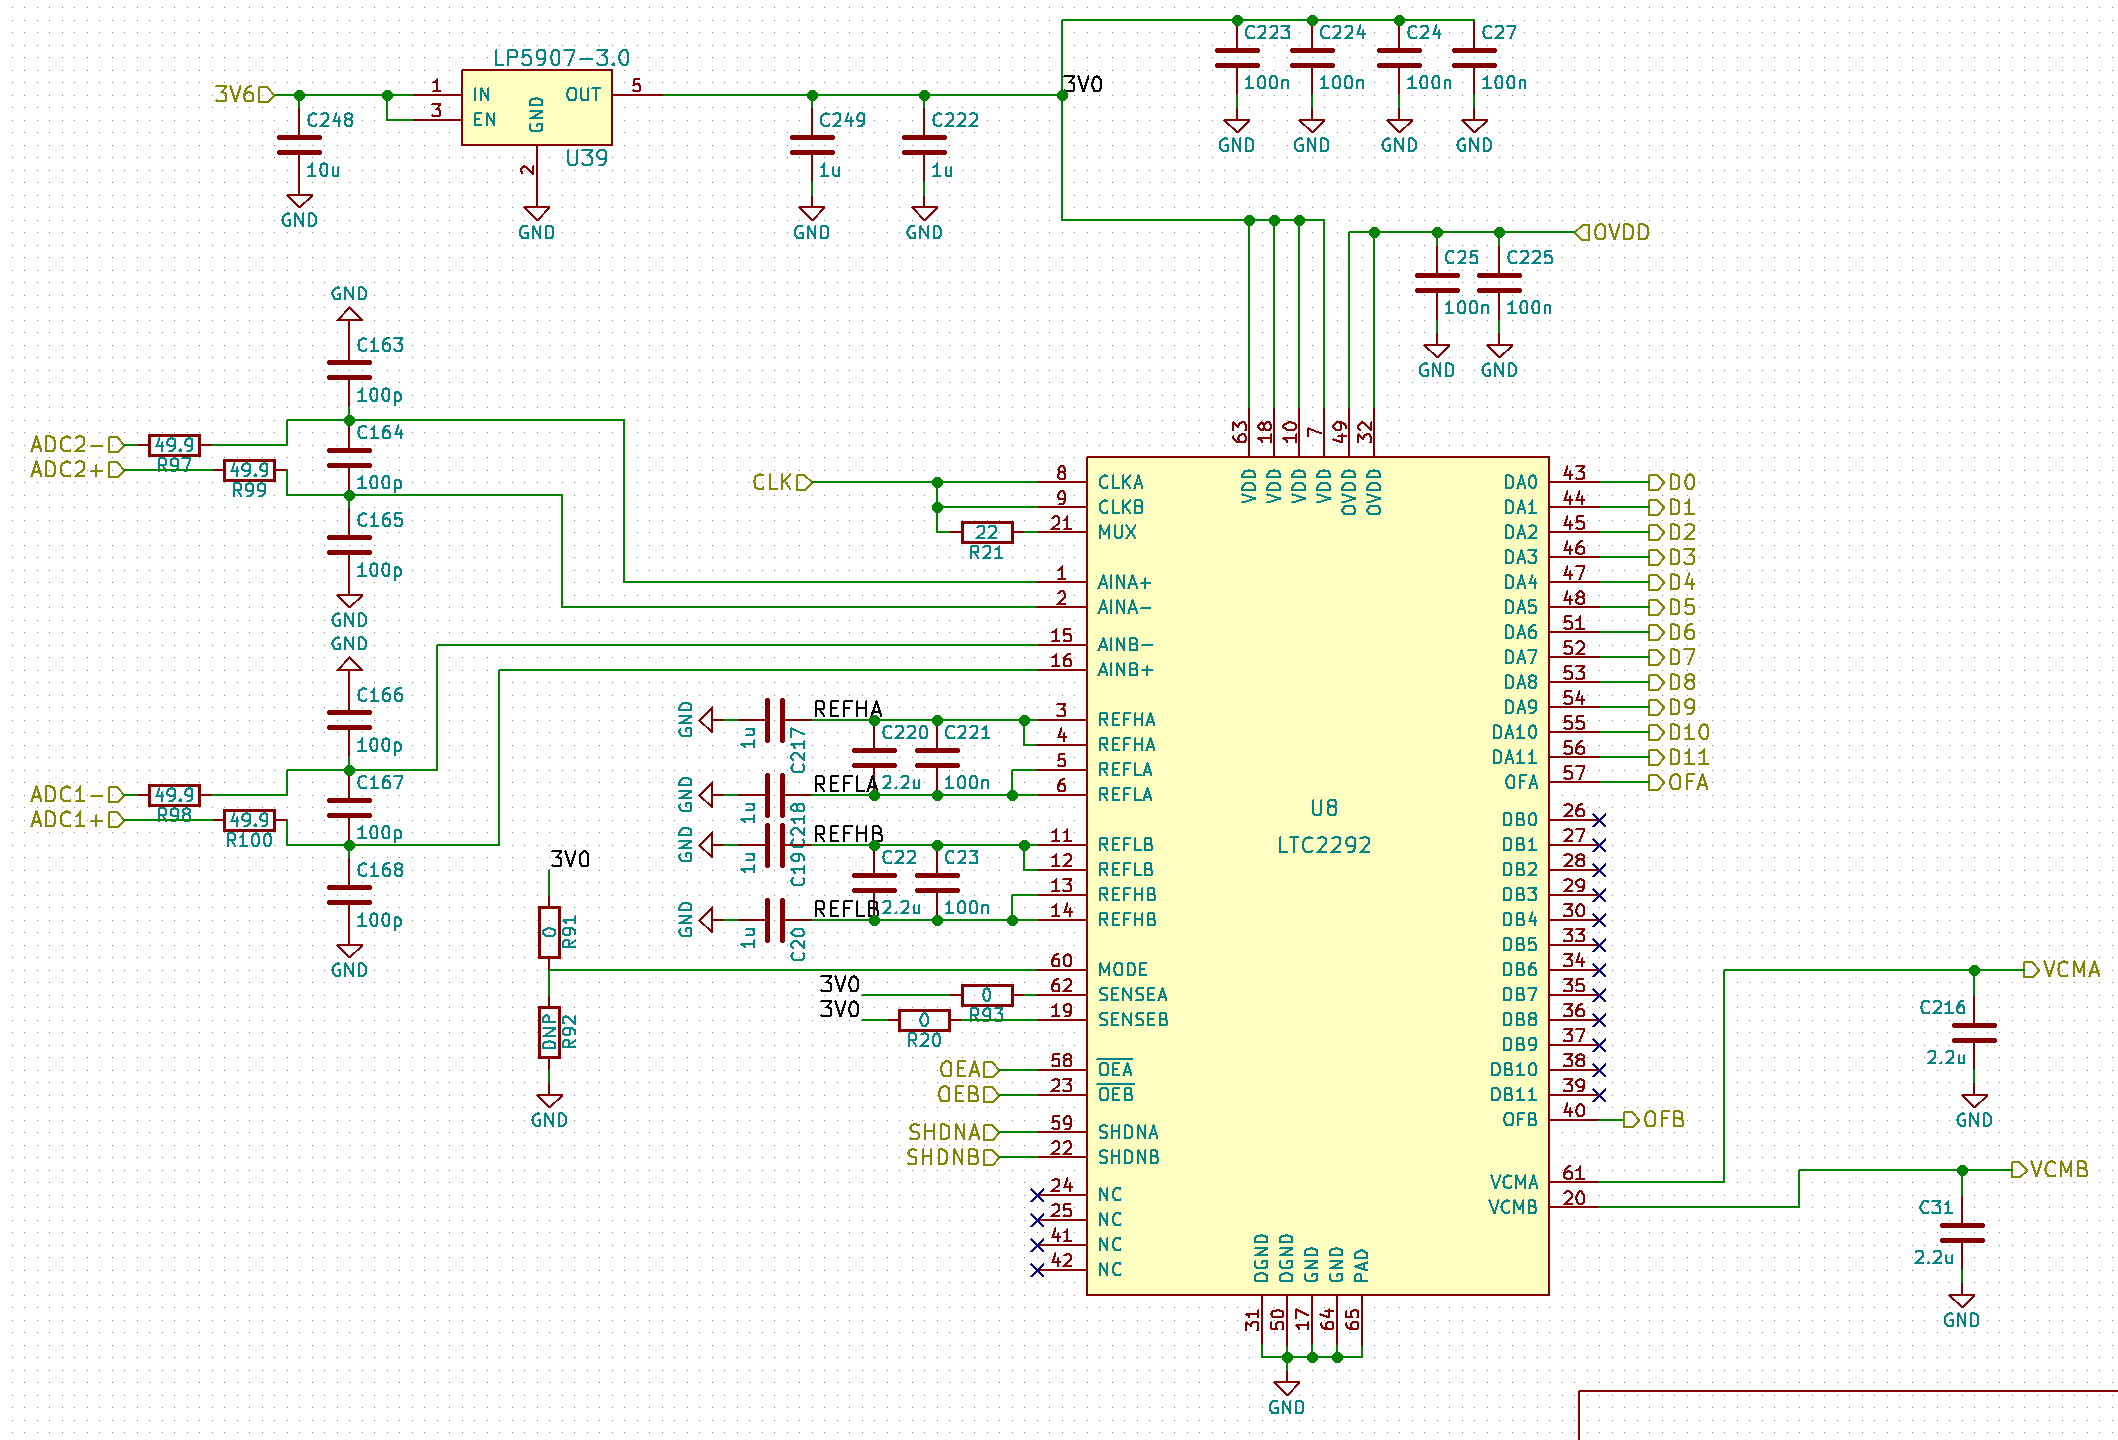
\includegraphics[width=\textwidth]{data/ltc2292-schematic.png}
  \caption{The LTC2292ADC schematic.}
  \label{fig:ltc2292-schematic}
\end{figure}

\begin{figure}[h]
  \centering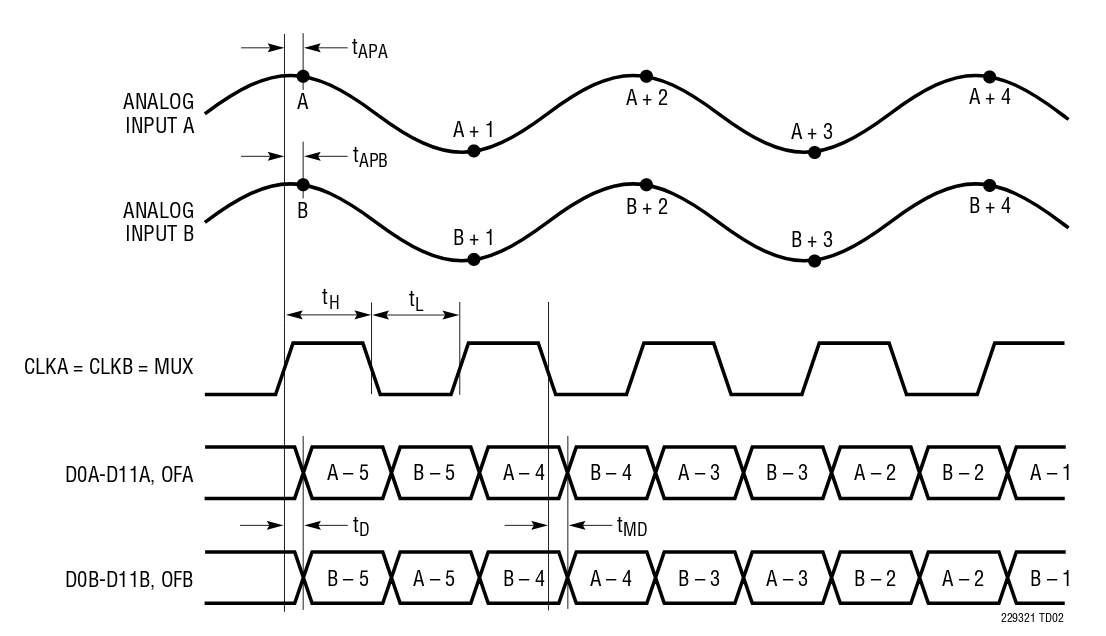
\includegraphics[width=0.75\textwidth]{data/LTC2292-multiplex.png}
  \caption{Multiplexed digital output bus timing for the LTC2292 ADC.}
  \label{fig:ltc2292-multiplex}
\end{figure}

\label{tab:ltc2292-pinout}
\begin{tabularx}{\textwidth}{>{\hsize=.25\hsize} X >{\hsize=.25\hsize} XX}
  \caption{All LTC2292 ADC pin connections in logical groupings.} \\
  \toprule\textbf{LABELS} & \textbf{PIN \#s} & \textbf{DESCRIPTION} \\
  \midrule
  \endhead

  VDD & 7, 10, 18, 63 & The power supply required is 3.0V and each pin requires its own 0.1$\mu$F
  capacitor. When designing the PCB, ensure that each capacitor is placed as close to its
  corresponding pin as possible to minimize the trace inductance. The 3.0V signal itself
  is generated by using an LP5907 LDO regulator that takes in a 3.6V signal.\\
  OVDD & 39, 42 & The power supply for the output that the ADC feeds to, which is the FPGA and takes
  a 3.3V power supply. So, we connect this to the 3.3V power rail and bypass it with two 0.1$\mu$F
  capacitors, one for each pin. Again, each should be placed adjacent to their corresponding pins
  (39 and 42). \\
  CLKA, CLKB, MUX & 8, 9, 21 & Feeds a 40MHz clock signal to the device and specifies that the
  digitized channel A and B data should be multiplexed and pass through both output buses A and
  B. We leave B unconnected, so only bus A matters. \\
  DA0-DA11 & 43-48, 51-56 & The digitized output data that contains the input data from both
  channels A and B, multiplexed. This is fed into the FPGA for processing. \\
  OFA & 57 & This pin is driven high when overflow or underflow occurs. Otherwise it is kept low. We
  export this to the FPGA, although it is not currently used by the FPGA logic. \\
  DB0-DB11 & 26-30, 33-39 & The channel B data bus. Since we multiplex everything through the
  channel A data bus, this data bus is redundant and therefore left unconnected. \\
  OFB & 40 & Similar to OFA, but for channel B. This is exported to the FPGA, but is also unused. \\
  VCMA, VCMB & 61, 20 & A 1.5V signal that is used to set the common-mode voltage of the IF
  differential amplifiers, whose outputs are sent to this ADC. They are each bypassed to GND with a
  2.2$\mu$F capacitor, which should be placed directly next to their respective pins. \\
  GND, OGND & 17, 64, 65, 31, 50 & The ADC power ground and output power ground, respectively. These
  can all be routed to the same ground plane. \\
  NC & 24-25, 41-42 & No connect. \\
  SHDNA, SHDNB, OEA, OEB & 59, 22, 58, 23 & These are input pins that are connected to the FPGA. The
  FPGA logic can ground both SHDNA and OEA to allow channel A to operate normally or bring them both
  high to put channel A in sleep mode. Channel B works the same way. \\
  SENSEA, SENSEB & 62, 19 & These are connected to VDD, which specifies that the input voltage range
  of the differential signals for both channels A and B is 1.5V $\pm$ 1V. 1.5V is the common-mode
  voltage and the channels allow a 2V range around that. \\
  MODE & 60 & Connecting mode to VDD specifies the output format as 2s complement and turns of the clock duty stabilizer, which is unnecessary because the input clock has a 50\% duty cycle. \\
  REFHA, REFLA, REFLB, REFHB & 3-6, 11-14 & These are the high and low reference for channels A and
  B, respectively. Their connection is specified exactly by the datasheet. It is critical that the
  0.1$\mu$F capacitor is placed as close to the pins as possible. \\
  AINA+, AINA-, AINB-, AINB+ & 1-2, 15-16 & The positive and negative differential inputs for
  channels A and B. \textbf{\{STARTINCOMPLETE\}} These lines have a capacitor between the positive
  and negative analog inputs, as well as capacitors connecting each line to GND. The capacitor value
  between the lines of 0.1$\mu$F is different from the suggested value of 12pF and the capacitors
  connecting the lines to GND are not suggested from the datasheet (see page 18 of the
  datasheet). Additionally, the resistance value of 49.9$\Omega$ differs from the suggested
  resistance of 25$\Omega$. Lastly, the negative output of the differential amplifier for channel
  Ais feeding into the positive input line \textbf{\{END INCOMPLETE\}}. \\

  \bottomrule
\end{tabularx}

\section{Mixer}
The mixer schematic shown in Figure~\ref{fig:mixer-sch} is composed of three high-frequency baluns
that convert two rx and one local oscillator (the original transmitted signal) single-ended signal
into differential signals and then feed them into the mixer. The baluns are
\href{https://www.johansontechnology.com/datasheets/baluns/Balun_5400BL15B050.pdf}{5400BL15B050E}
and the mixer is
\href{http://www.analog.com/media/en/technical_documentation/data_sheets/ADL5802.pdf}{ADL5802}. The
mixer outputs the difference of the local oscillator frequency and each R input which ranges from
hundreds of kHz to a few MHz.

\begin{figure}[ht]
  \centering
  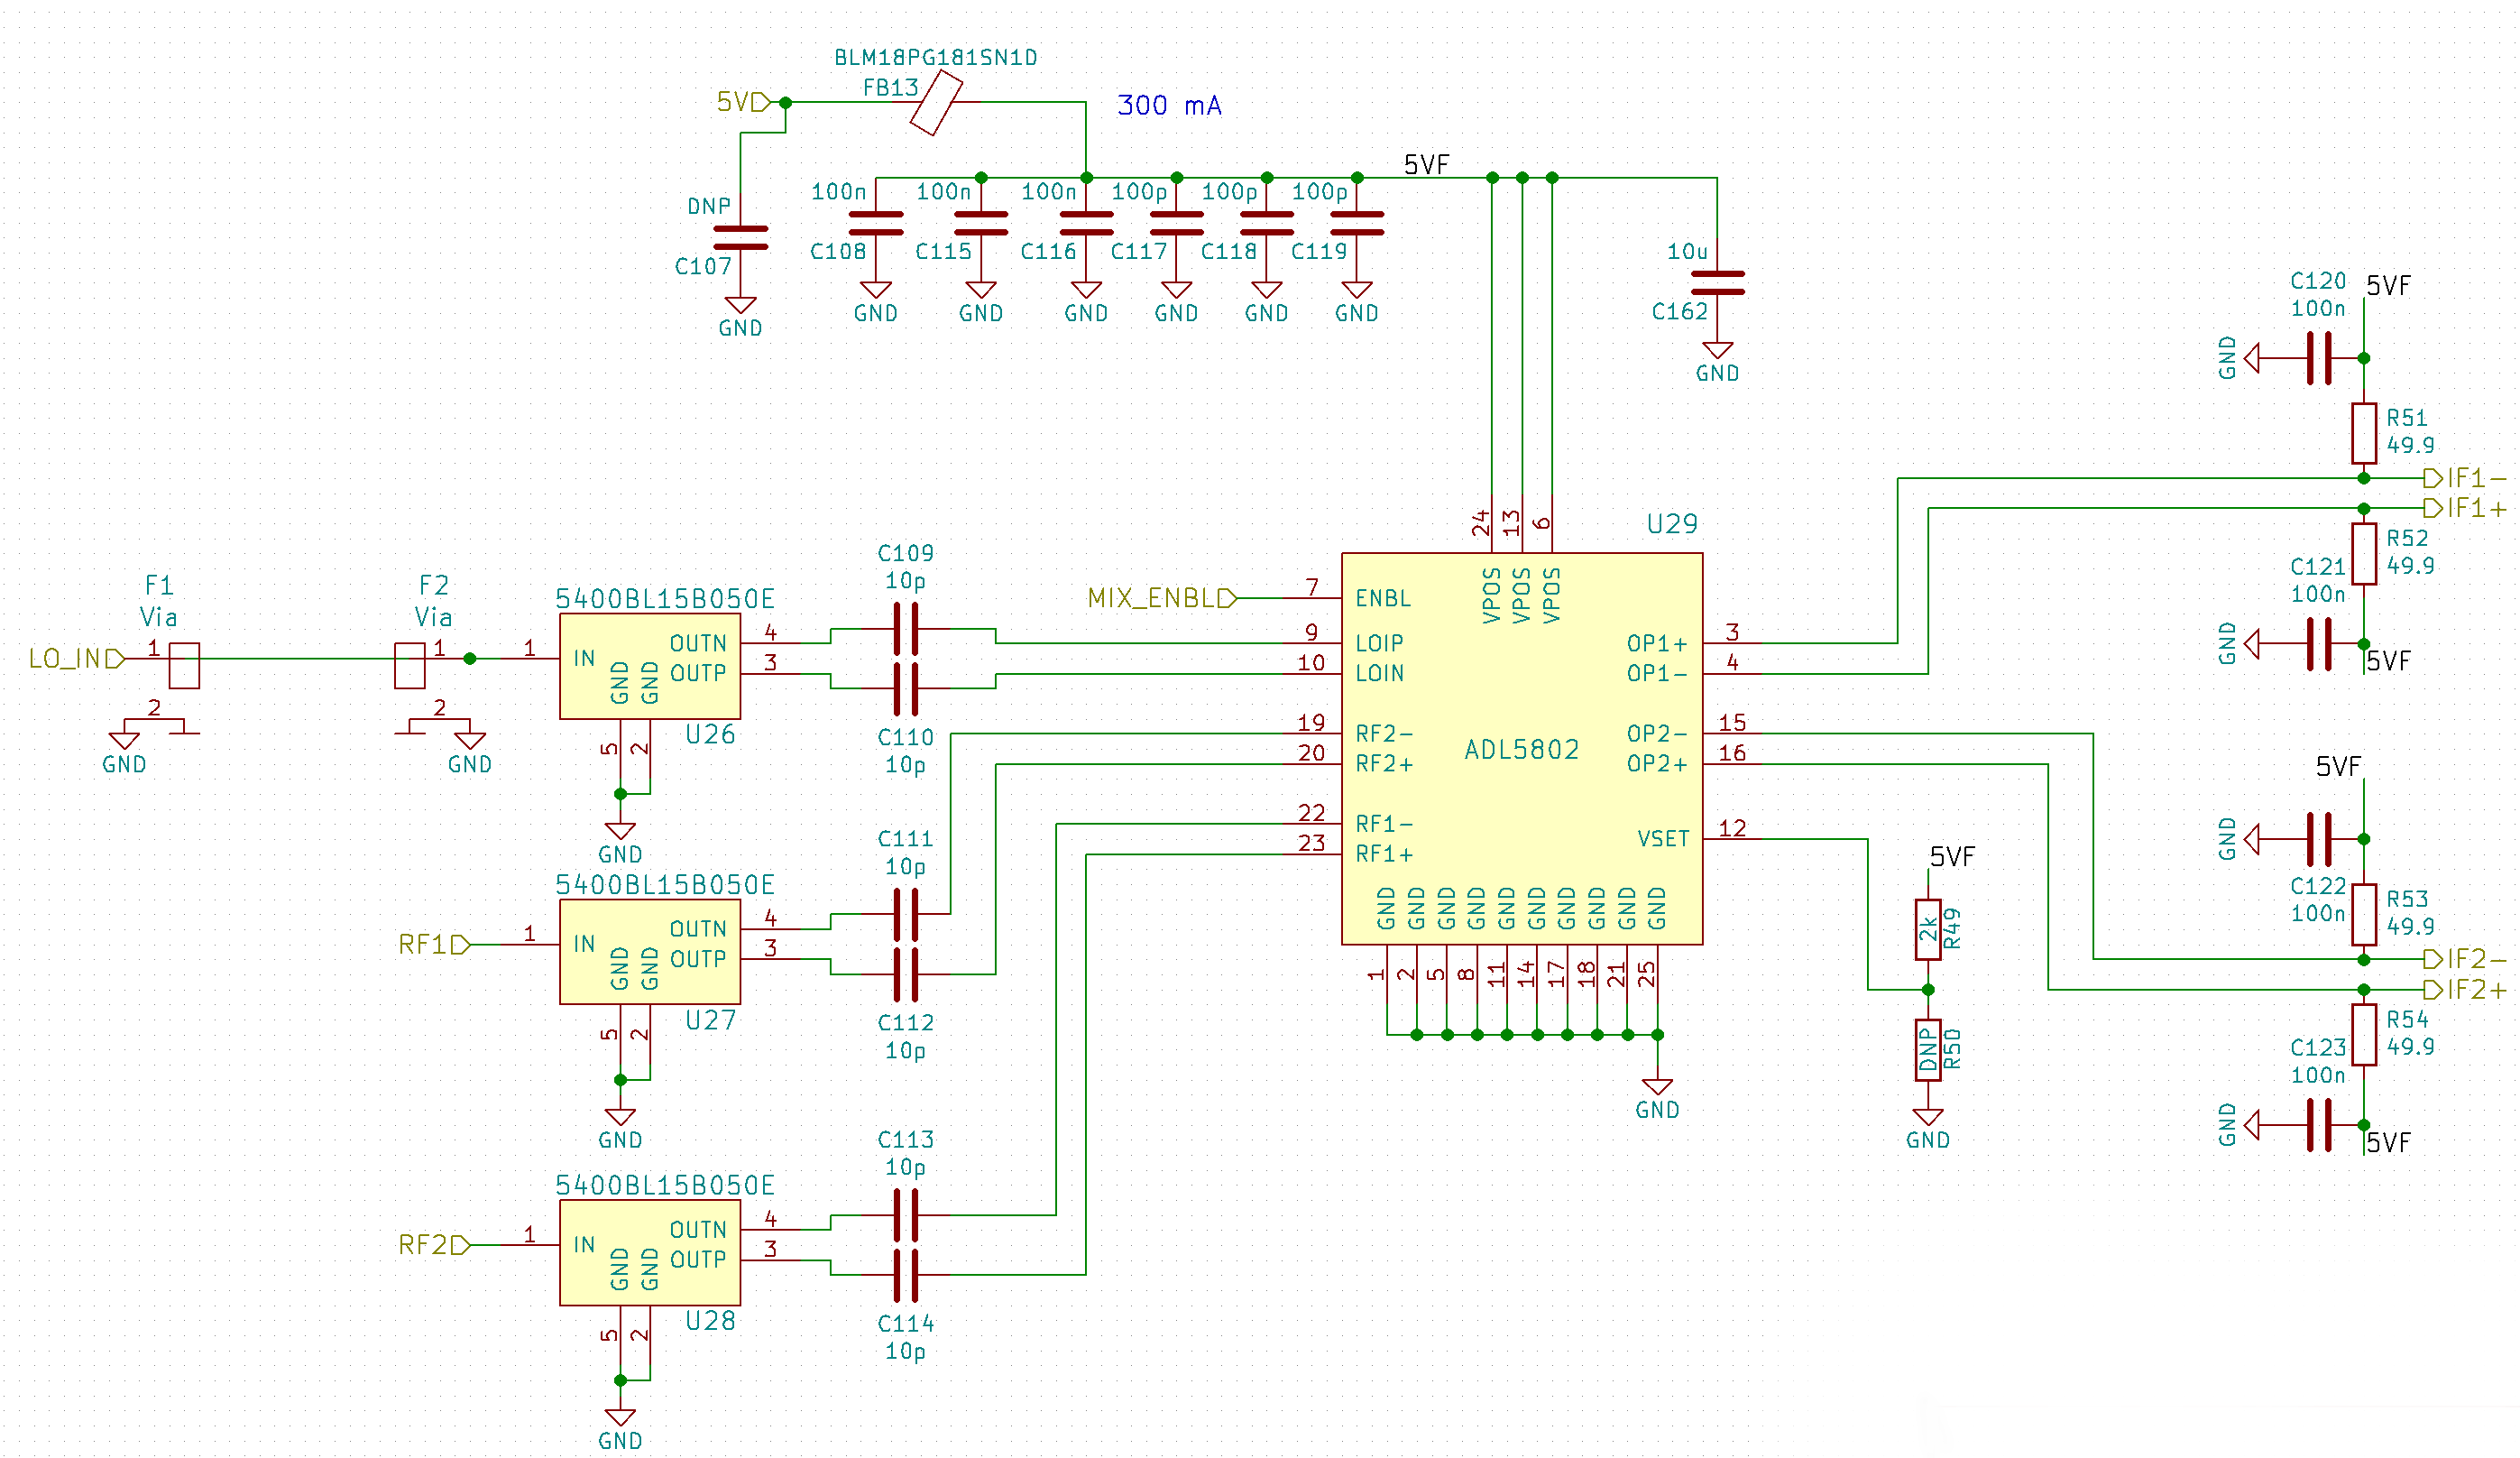
\includegraphics[width=\textwidth]{data/mixer-sch.png}
  \caption{The mixer schematic.}
  \label{fig:mixer-sch}
\end{figure}

The RF and LO input interfaces are designed for a differential input impedance of 50$\Omega$. This
is already the differential balanced impedance of the baluns, so we do not need to perform any
additional impedance matching at the inputs. The inputs require AC coupling and the datasheet
recommends 3pF coupling capacitors placed between the balun outputs and pin inputs. It also shows
that the positive balun output of the local oscillator should be hooked up to the positive pin
input.

\section{IF}

The IF amplifier,
\href{http://www.analog.com/media/en/technical-documentation/data-sheets/ADA4940-1_4940-2.pdf}{ADA4940-2},
receives the output of the mixer, whose frequency is in the range of hundreds of kHz to a few MHz.

\section{RX1 \& RX2}

The sheets RX1 and RX2 are identical. They each consist of two amplifiers connected in series, shown
in Figure~\ref{fig:rx-sch}. The first amplifier is a
\href{http://www.skyworksinc.com/uploads/documents/SKY65404_31_201512J.pdf}{SKY65404} LNA which
operates in the 4.9GHz-5.9GHz range, has a gain of 13dB, a NF of 1dB and a P1dB of -4dBm. It is
hooked up exactly as specified in the datasheet, with the addition of a ferrite bead filtering its
power supply.

\begin{figure}[h]
  \centering
  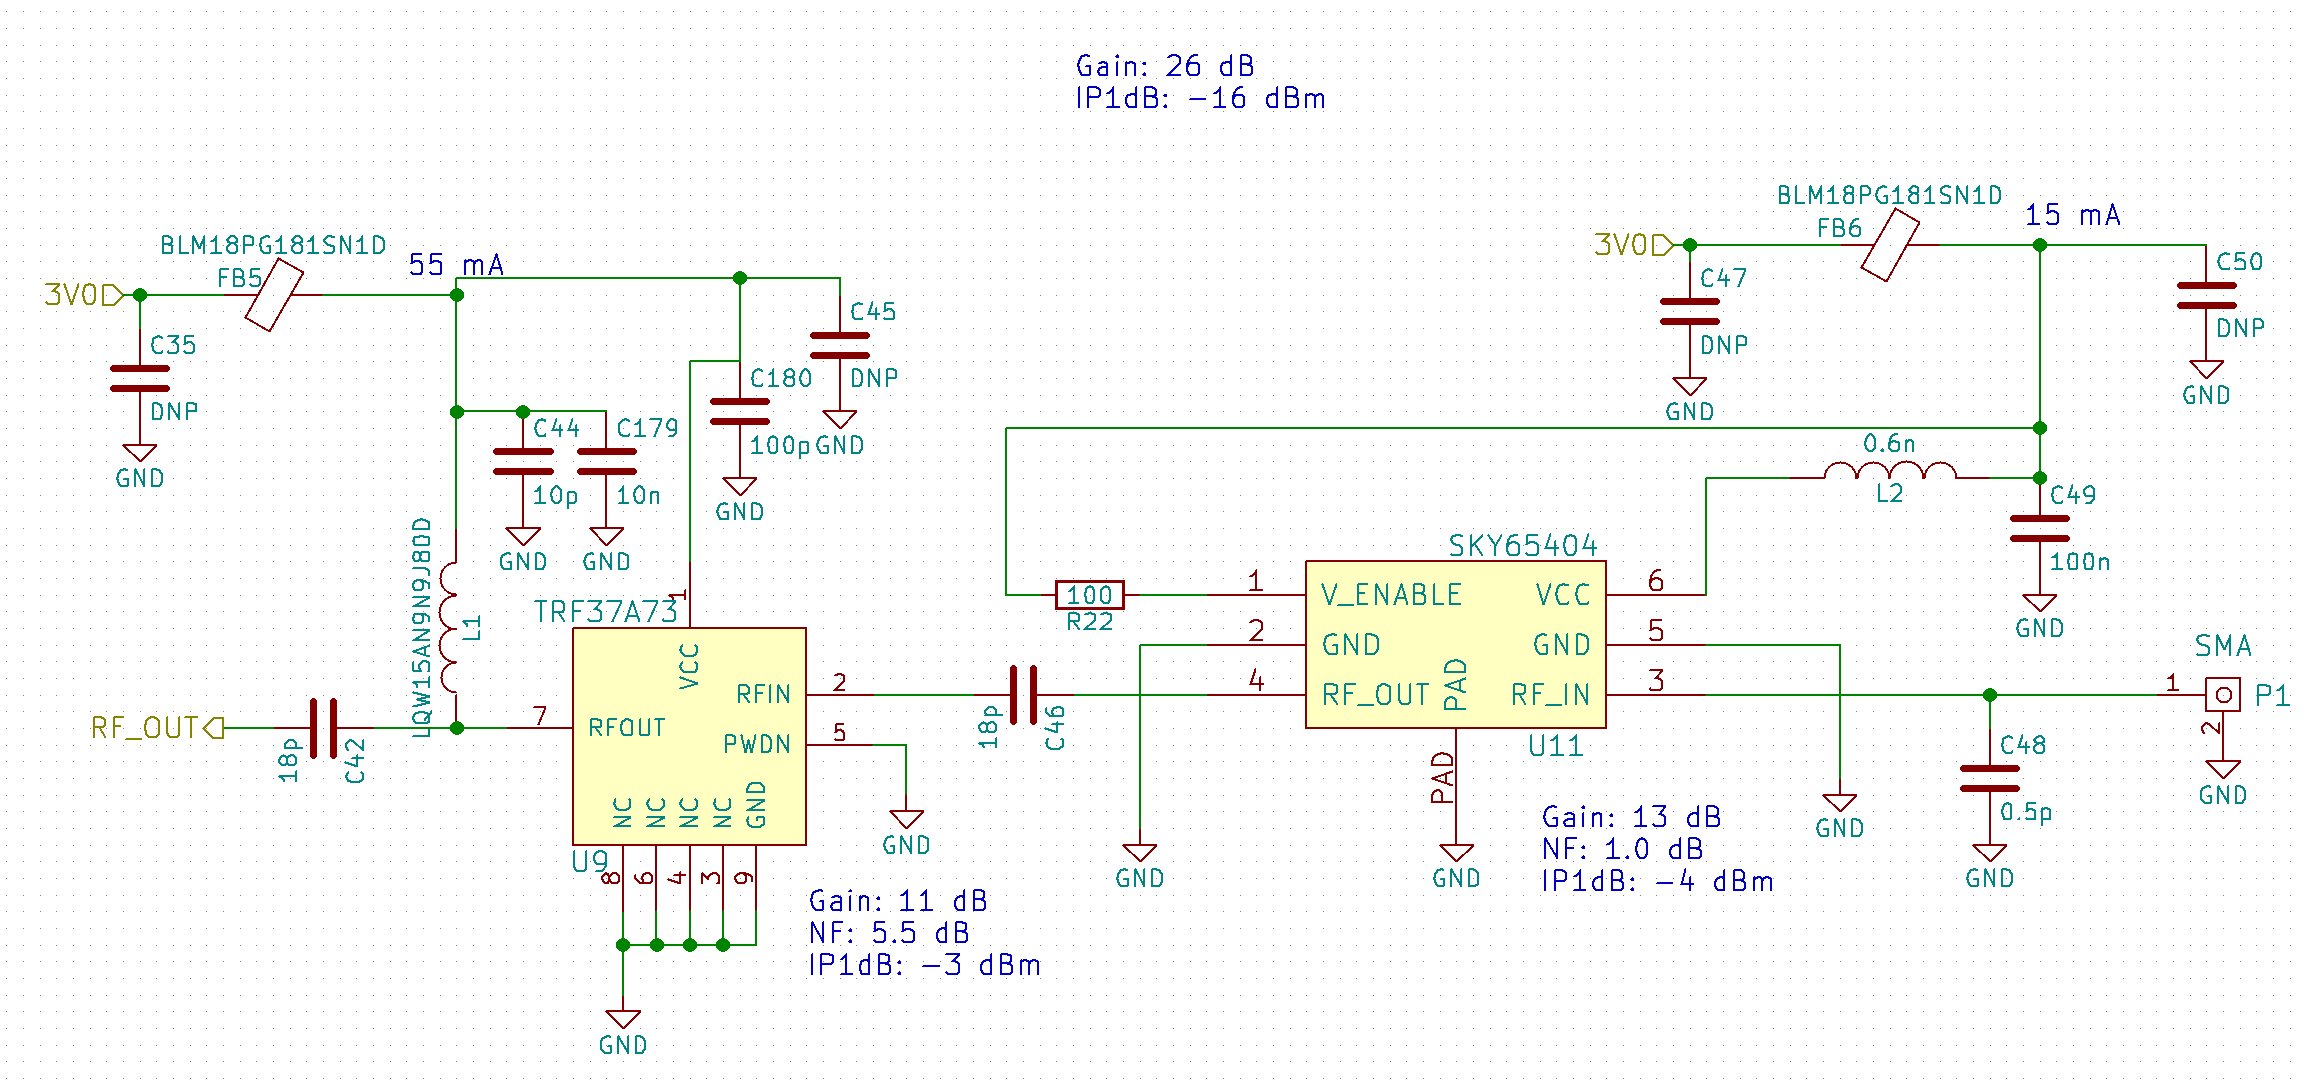
\includegraphics[width=\textwidth]{data/rx-sch.png}
  \caption{One of two RX schematic sheets. Both sheets are identical and consist of two amplifiers
    connected in series.}
  \label{fig:rx-sch}
\end{figure}

The second amplifier is a \href{http://www.ti.com/lit/ds/symlink/trf37a73.pdf}{TRF37A73} RF gain
amplifier. It is wired up as recommended in the datasheet, with the addition of a ferrite bead to
filter the power supply. Values for the various capacitors and inductor are left out of the
datasheet. A 100pF capacitor is used to short high frequency noise to the power supply, which is
typical of microwave devices. \textbf{\{START INCOMPLETE\}} I am not sure how the values for the RF
bypass capacitors, the inductor, and the DC blocking capacitors was chosen. Additionally, I'm not
sure how he arrives at a gain of 26dB, since I've read that gains in series should be additive (and
hence 24dB), and I'm not sure where the IP1dB value of -16dBm comes from \textbf{\{ENDINCOMPLETE\}}.

\chapter{PCB}
\section{General Layout}

The radar is constructed using a 4-layer board and uses both surfaces of the board. The front layer
contains nearly all of the board's components while the back layer contains a few surface mount
resistors and capacitors. The top layer primarily contains signal traces for top layer SMD
components. In particular, it connects many of the signal traces of the ADC to the FPGA, which is
placed next to it. Note, however, that most of the signal traces extending from the FPGA only start
on the top layer but travel through layer 3. The buck converters and subsequent linear regulators
are placed near the top of the board, not necessarily near the components they drive. In addition to
the large number of signal traces, the top copper layer contains a large ground plane around the
periphery of the board. The 2nd layer is entirely a ground plane. The 3rd layer is largely a ground
plane, although it also contains a significant number of traces extending from the FPGA as well as a
few other components. The 4th layer primarily contains large power planes for each of the different
voltages driving logic in the design. It is worth noting that even though it contains significant
power planes, it still has a ground plane that is the largest copper fill zone in this layer. The
PCB also has 3 large corner mounting vias with smaller vias placed in a circle in the large via's
annular ring. The reason for the small vias is to ensure a continued connection to GND (the mounting
vias are connected to GND) even if a screw thread strips too much copper from the main
via. Additionally, it helps prevent the PCB from being crushed if too much torque is used to tighten
the screw. The 4th corner is occupied by the connections to the DC barrel jack. Power rail tracesare
made 0.5mm in width whereas signal traces are 0.2mm in width. Grounded vias are placed liberally
throughout the design. They have a diameter of 0.46mm and a drill hole size of 0.254mm. I've included
several screenshots of the PCB and highlighted important
components (Figures~\ref{fig:fmcw-layer1-layout}, ~\ref{fig:fmcw-layer1-gnd},
~\ref{fig:fmcw-layer2-gnd}, ~\ref{fig:fmcw-layer3-gnd}, ~\ref{fig:fmcw-layer4-gnd},
~\ref{fig:fmcw-layer4-12v}, ~\ref{fig:fmcw-layer4-3v6}, ~\ref{fig:fmcw-layer4-3v0},
~\ref{fig:fmcw-layer4-3v3a}, ~\ref{fig:fmcw-layer4-3v3d}, ~\ref{fig:fmcw-layer4-5v},
~\ref{fig:fmcw-layer4-5vf}).

\begin{figure}[h]
  \centering
  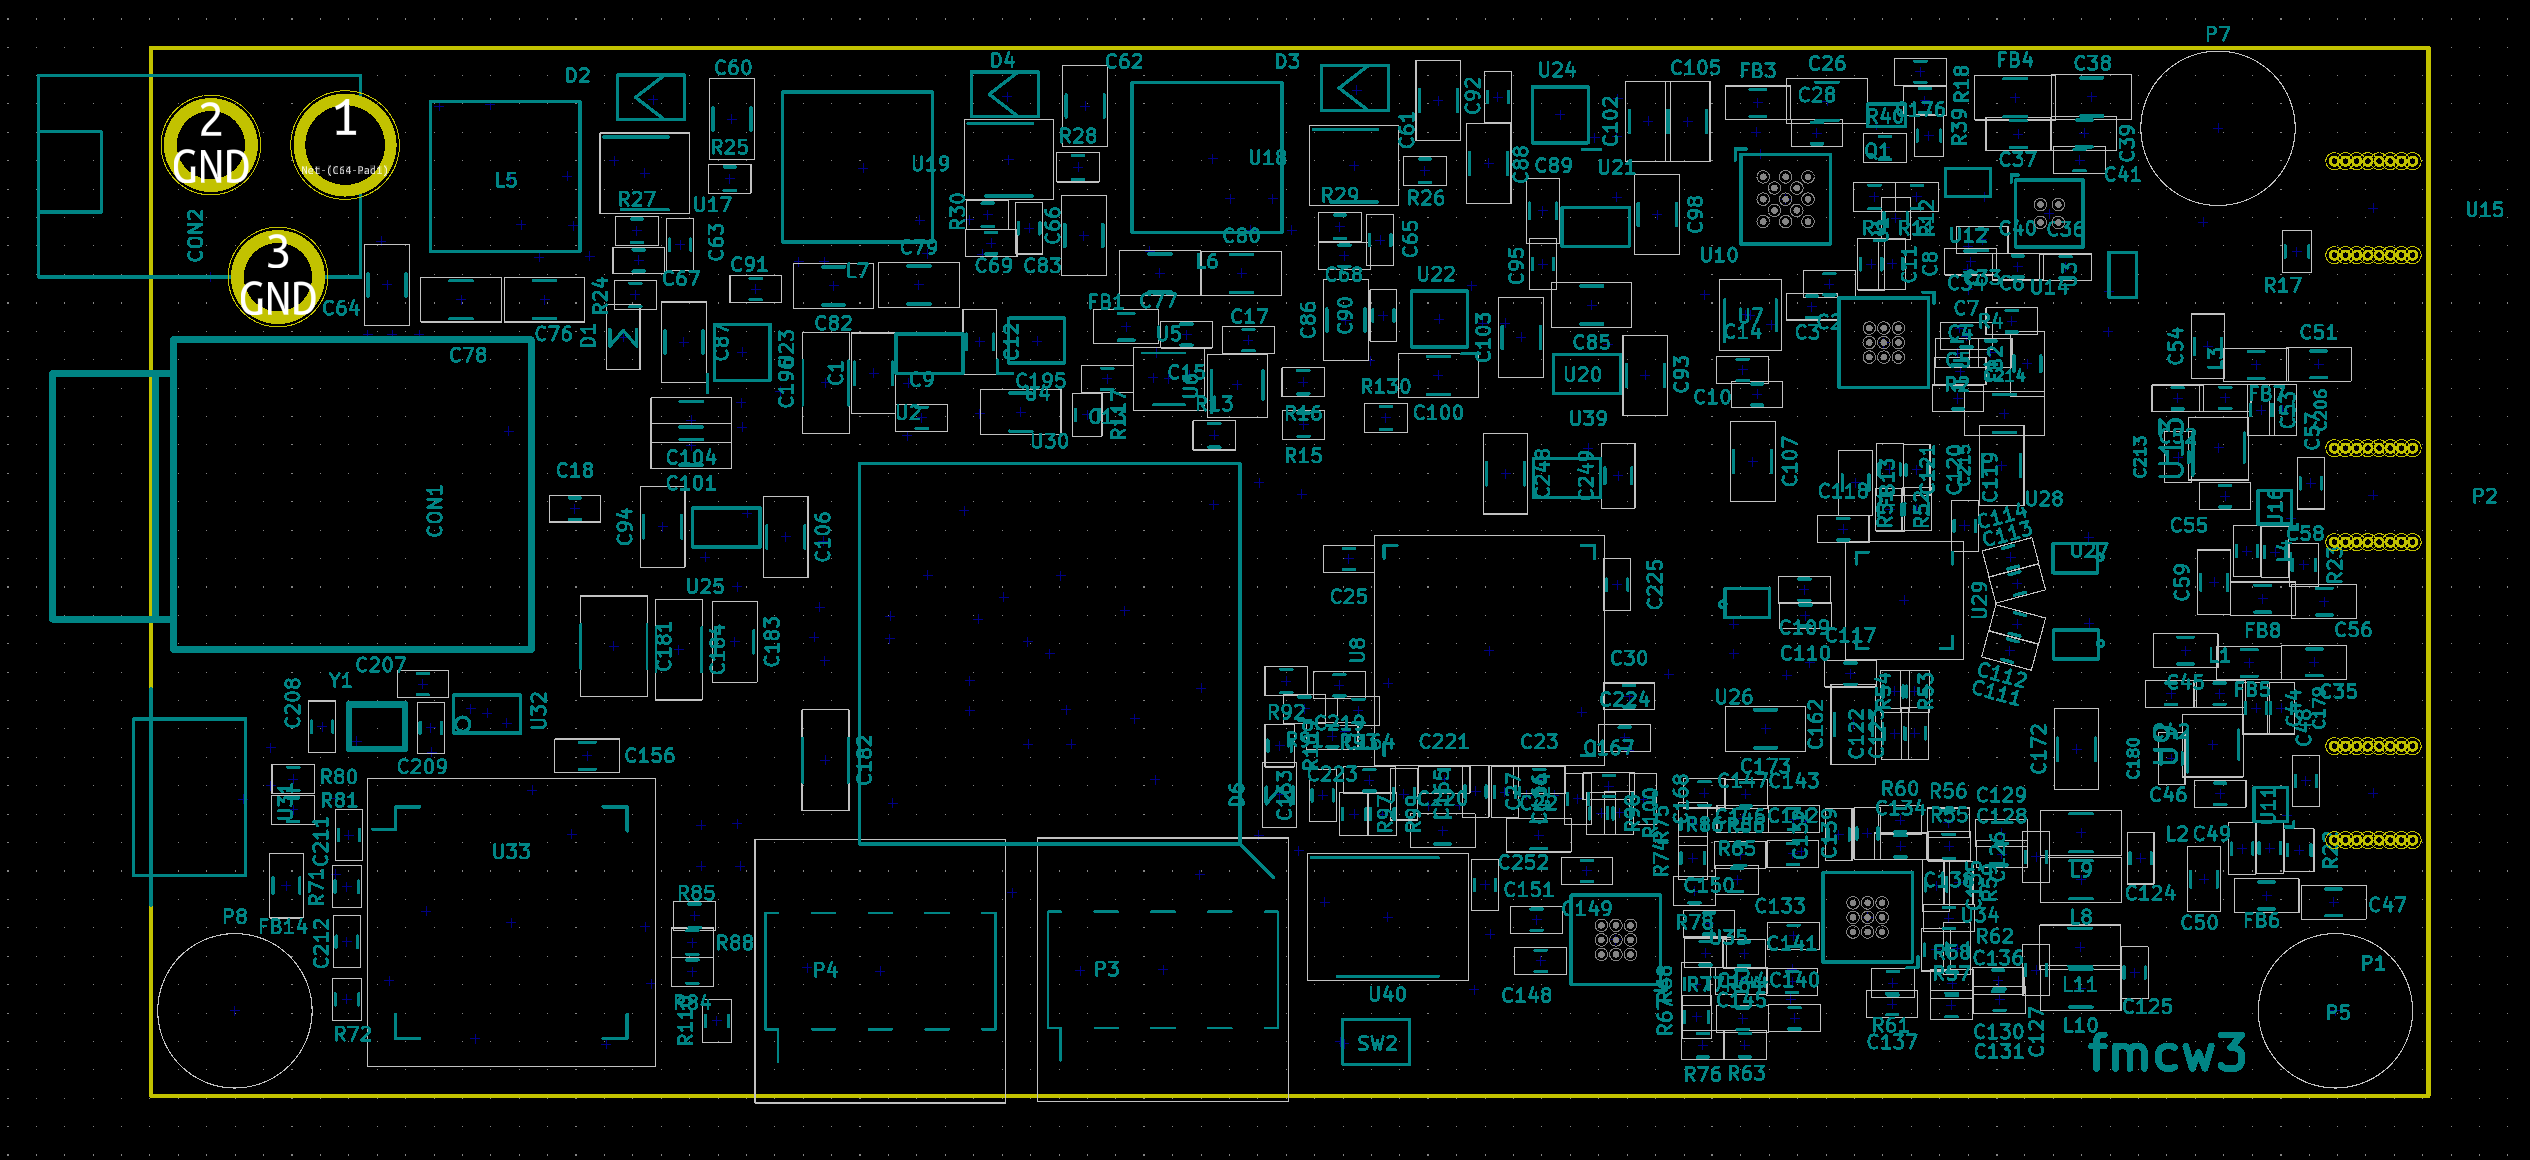
\includegraphics[width=\textwidth]{data/fmcw-layer1-layout.png}
  \caption{\textbf{Board layout}. The top left of the board is where the power source (barrel jack)
    is connected. The output of the 12V power source is connected to a power plane at the top
    left-middle of the board, that feeds into the buck converters. Large inductors connected to the
    buck converters are placed adjacent to their corresponding buck converters. The outputs of the
    buck converters feed into linear regulators that are mostly placed directly below the buck
    converters. This is also the region where the main crystal oscillator is placed and its
    associated fan-out buffer. Transmission circuitry (the frequency synthesizer and some RF
    amplifiers) are placed at the upper right side of the board near the antenna connectors which
    are placed on the right side of the board. Circuitry for signal reception are placed along the
    right side, adjacent to the antenna connectors. The mixer is placed slight inward from here,
    vertically centered but toward the right side of the board. Below this are intermediate
    frequency op-amps that feed the mixed signal into an ADC located just above it and to the left
    (U8). Located just to the left of the IF amplifiers and below the ADC is a flash memory IC (U40)
    which feeds data to the FPGA (U30), located just to the left of the ADC. Connectors below the
    FPGA (P3 and P4) can be used to externally monitor the FPGA. In the bottom left of the board is
    a component to convert USB data to UART data to configure the FPGA as well as a micro USB
    connection to connect to a host computer. On the left side of the board between the USB
    connection and barrel jack is a SD card reader that stores data that can be read back out the
    FPGA.}
  \label{fig:fmcw-layer1-layout}
\end{figure}

\begin{figure}[h]
  \centering
  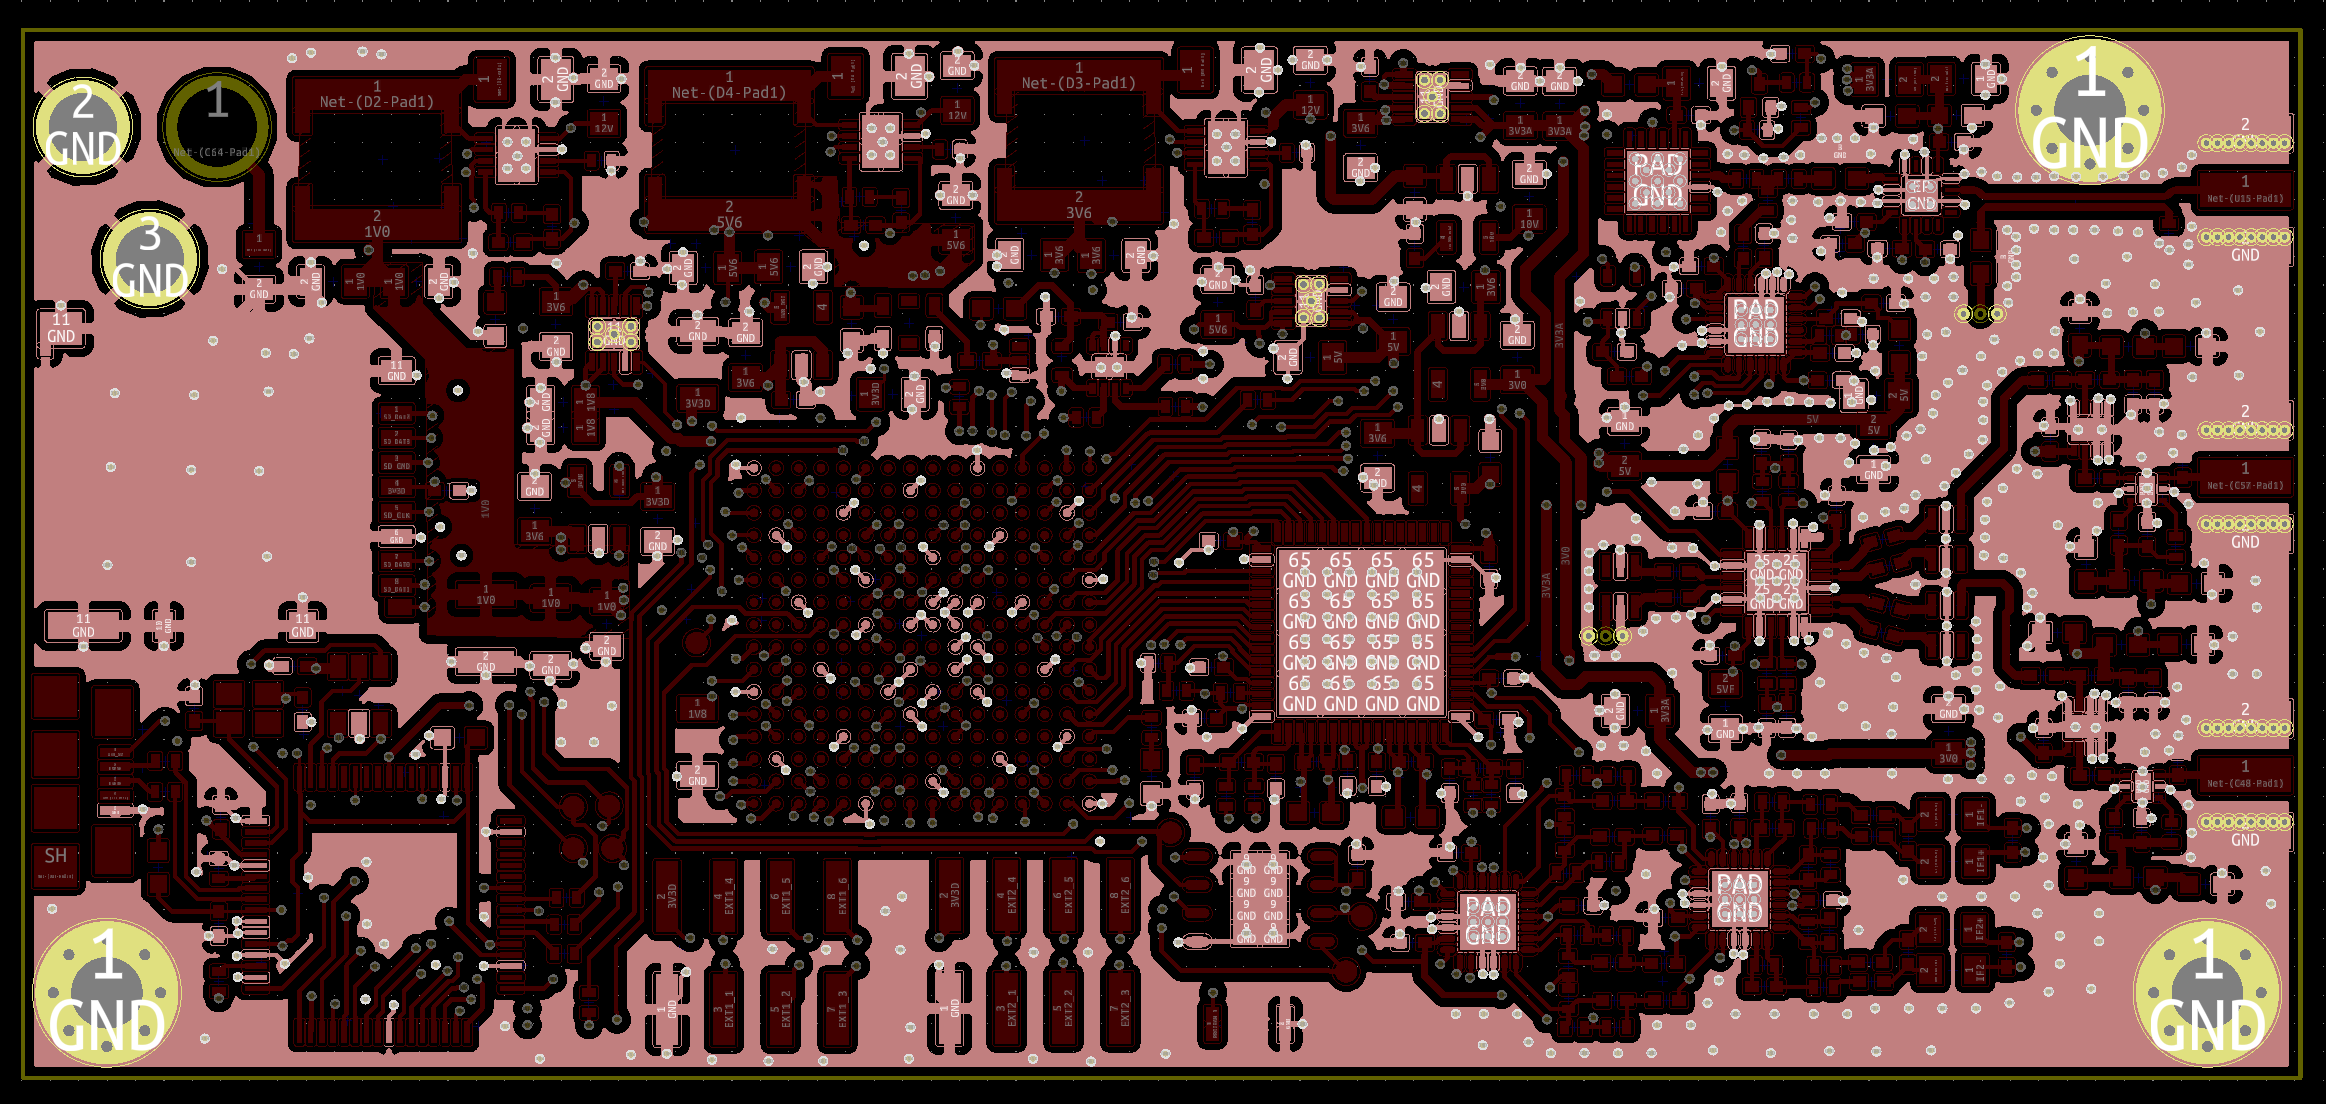
\includegraphics[width=\textwidth]{data/fmcw-layer1-gnd.png}
  \caption{A significant portion of layer 1 is a ground plane and the other large part of it is
    signal traces connecting components. There is also a small 1V power plane toward the upper left
    not highlighted here.}
  \label{fig:fmcw-layer1-gnd}
\end{figure}

\begin{figure}[h]
  \centering
  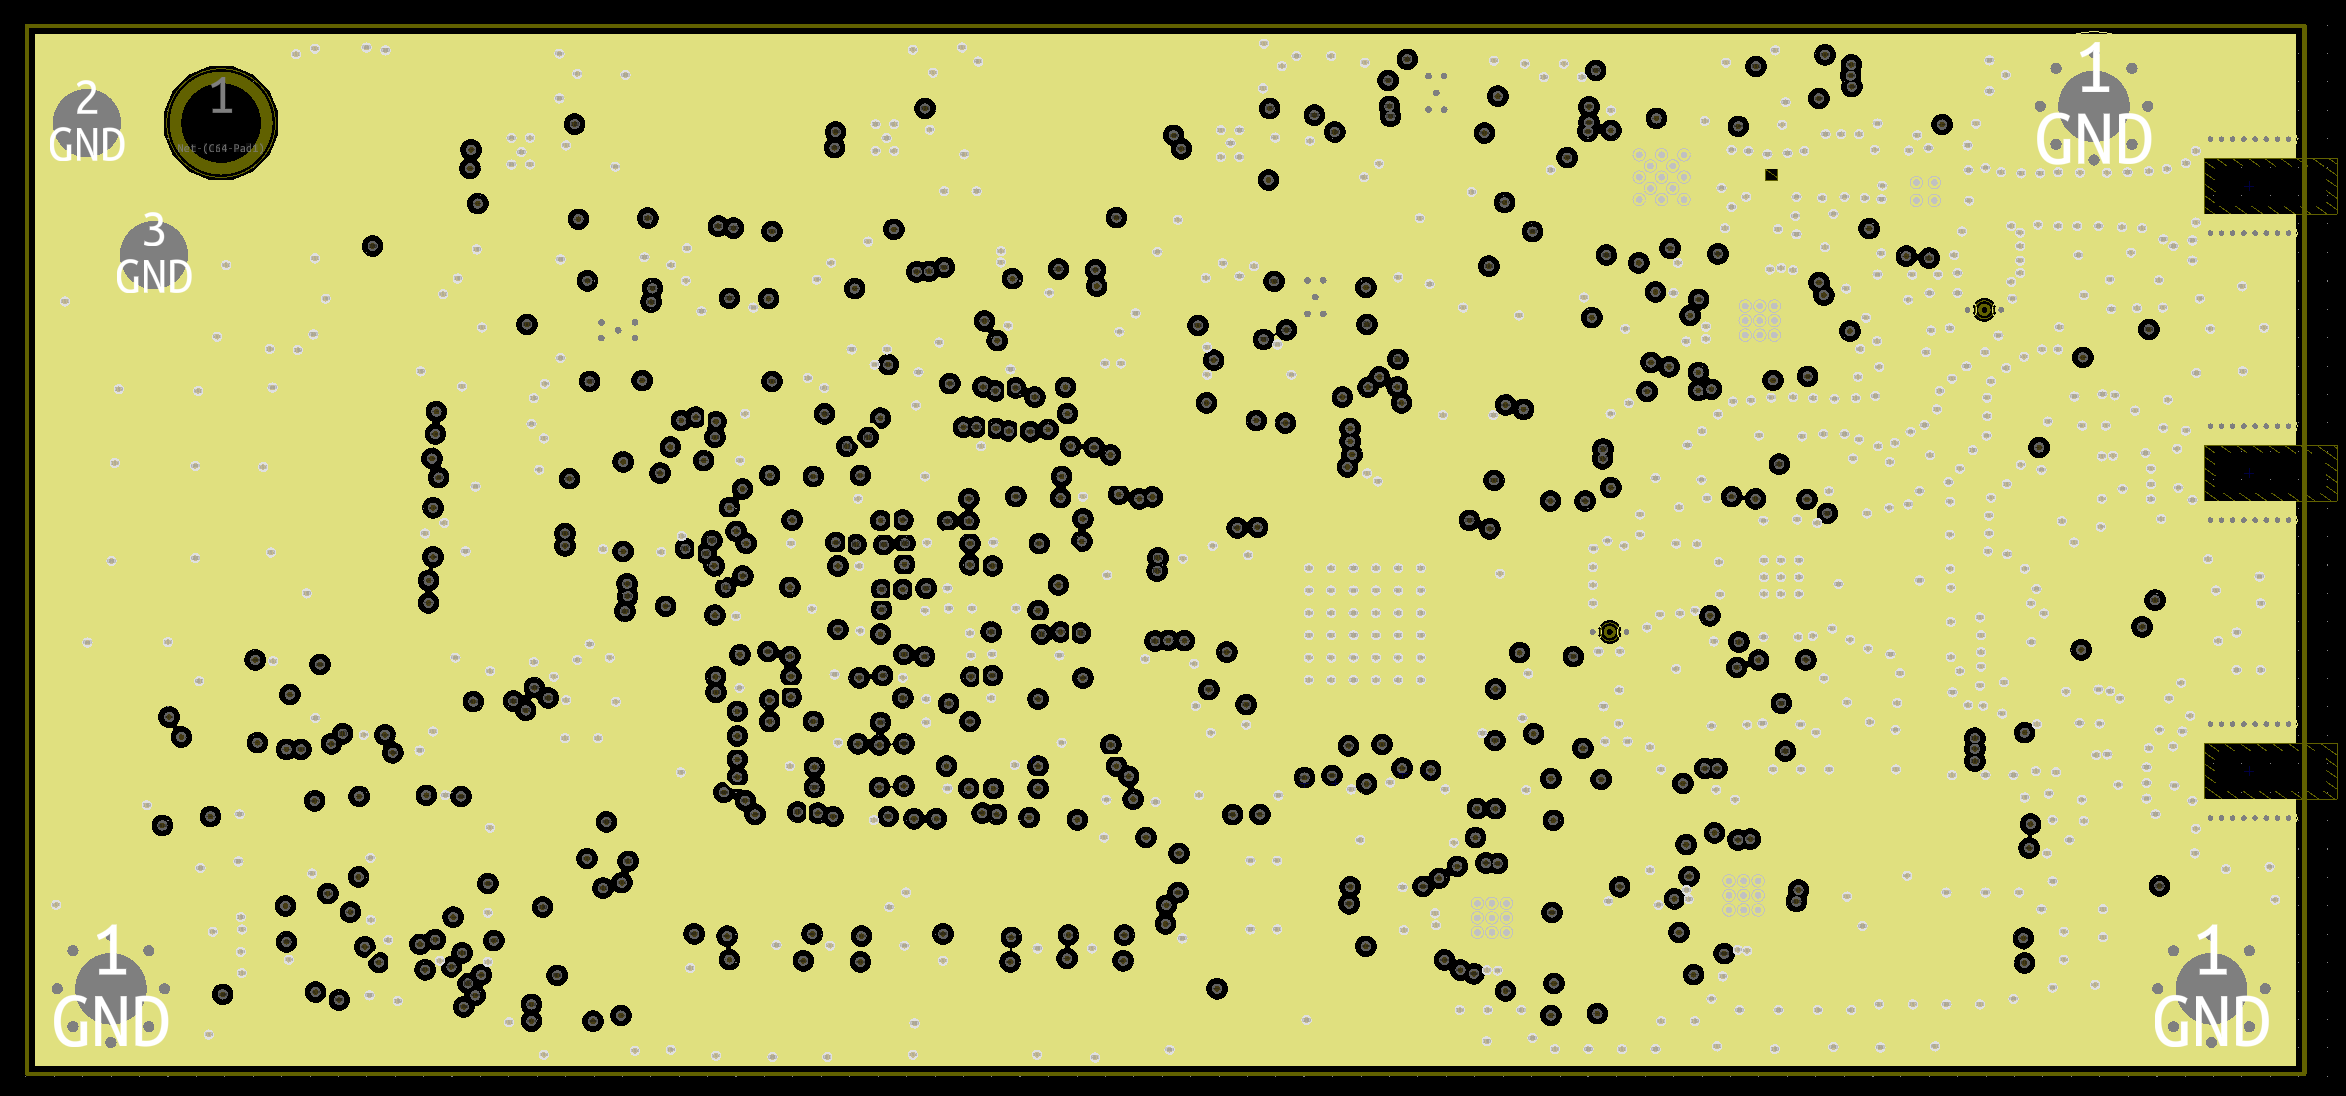
\includegraphics[width=\textwidth]{data/fmcw-layer2-gnd.png}
  \caption{All of layer 2 is a ground plane.}
  \label{fig:fmcw-layer2-gnd}
\end{figure}

\begin{figure}[h]
  \centering
  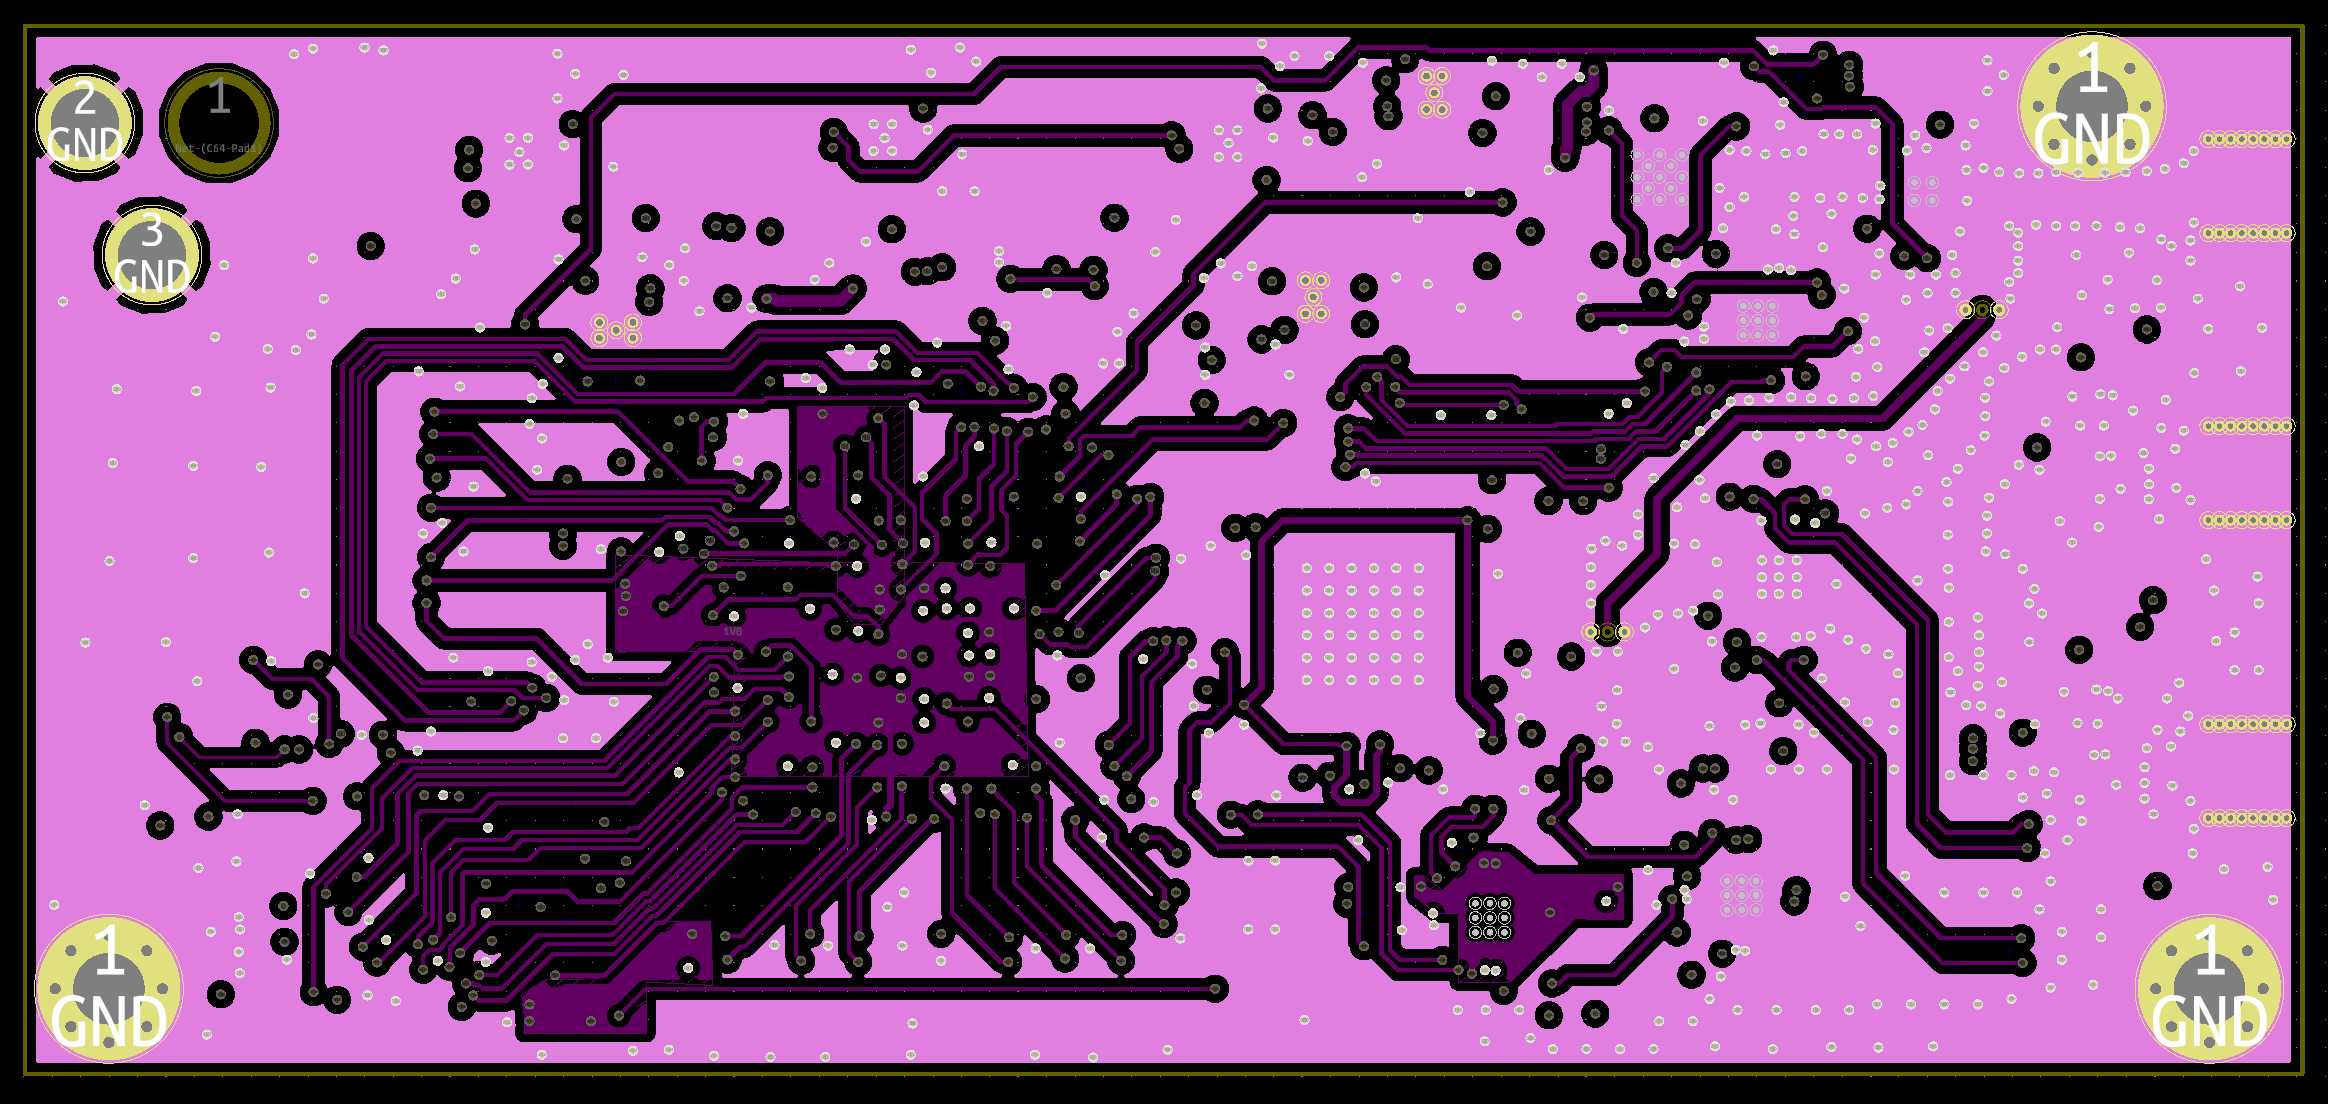
\includegraphics[width=\textwidth]{data/fmcw-layer3-gnd.png}
  \caption{Most of layer 3 is a ground plane but there are also a substantial number of trace
    connecting to the FPGA. It does also contain 1V an 3.3V power planes.}
  \label{fig:fmcw-layer3-gnd}
\end{figure}

\begin{figure}[h]
  \centering
  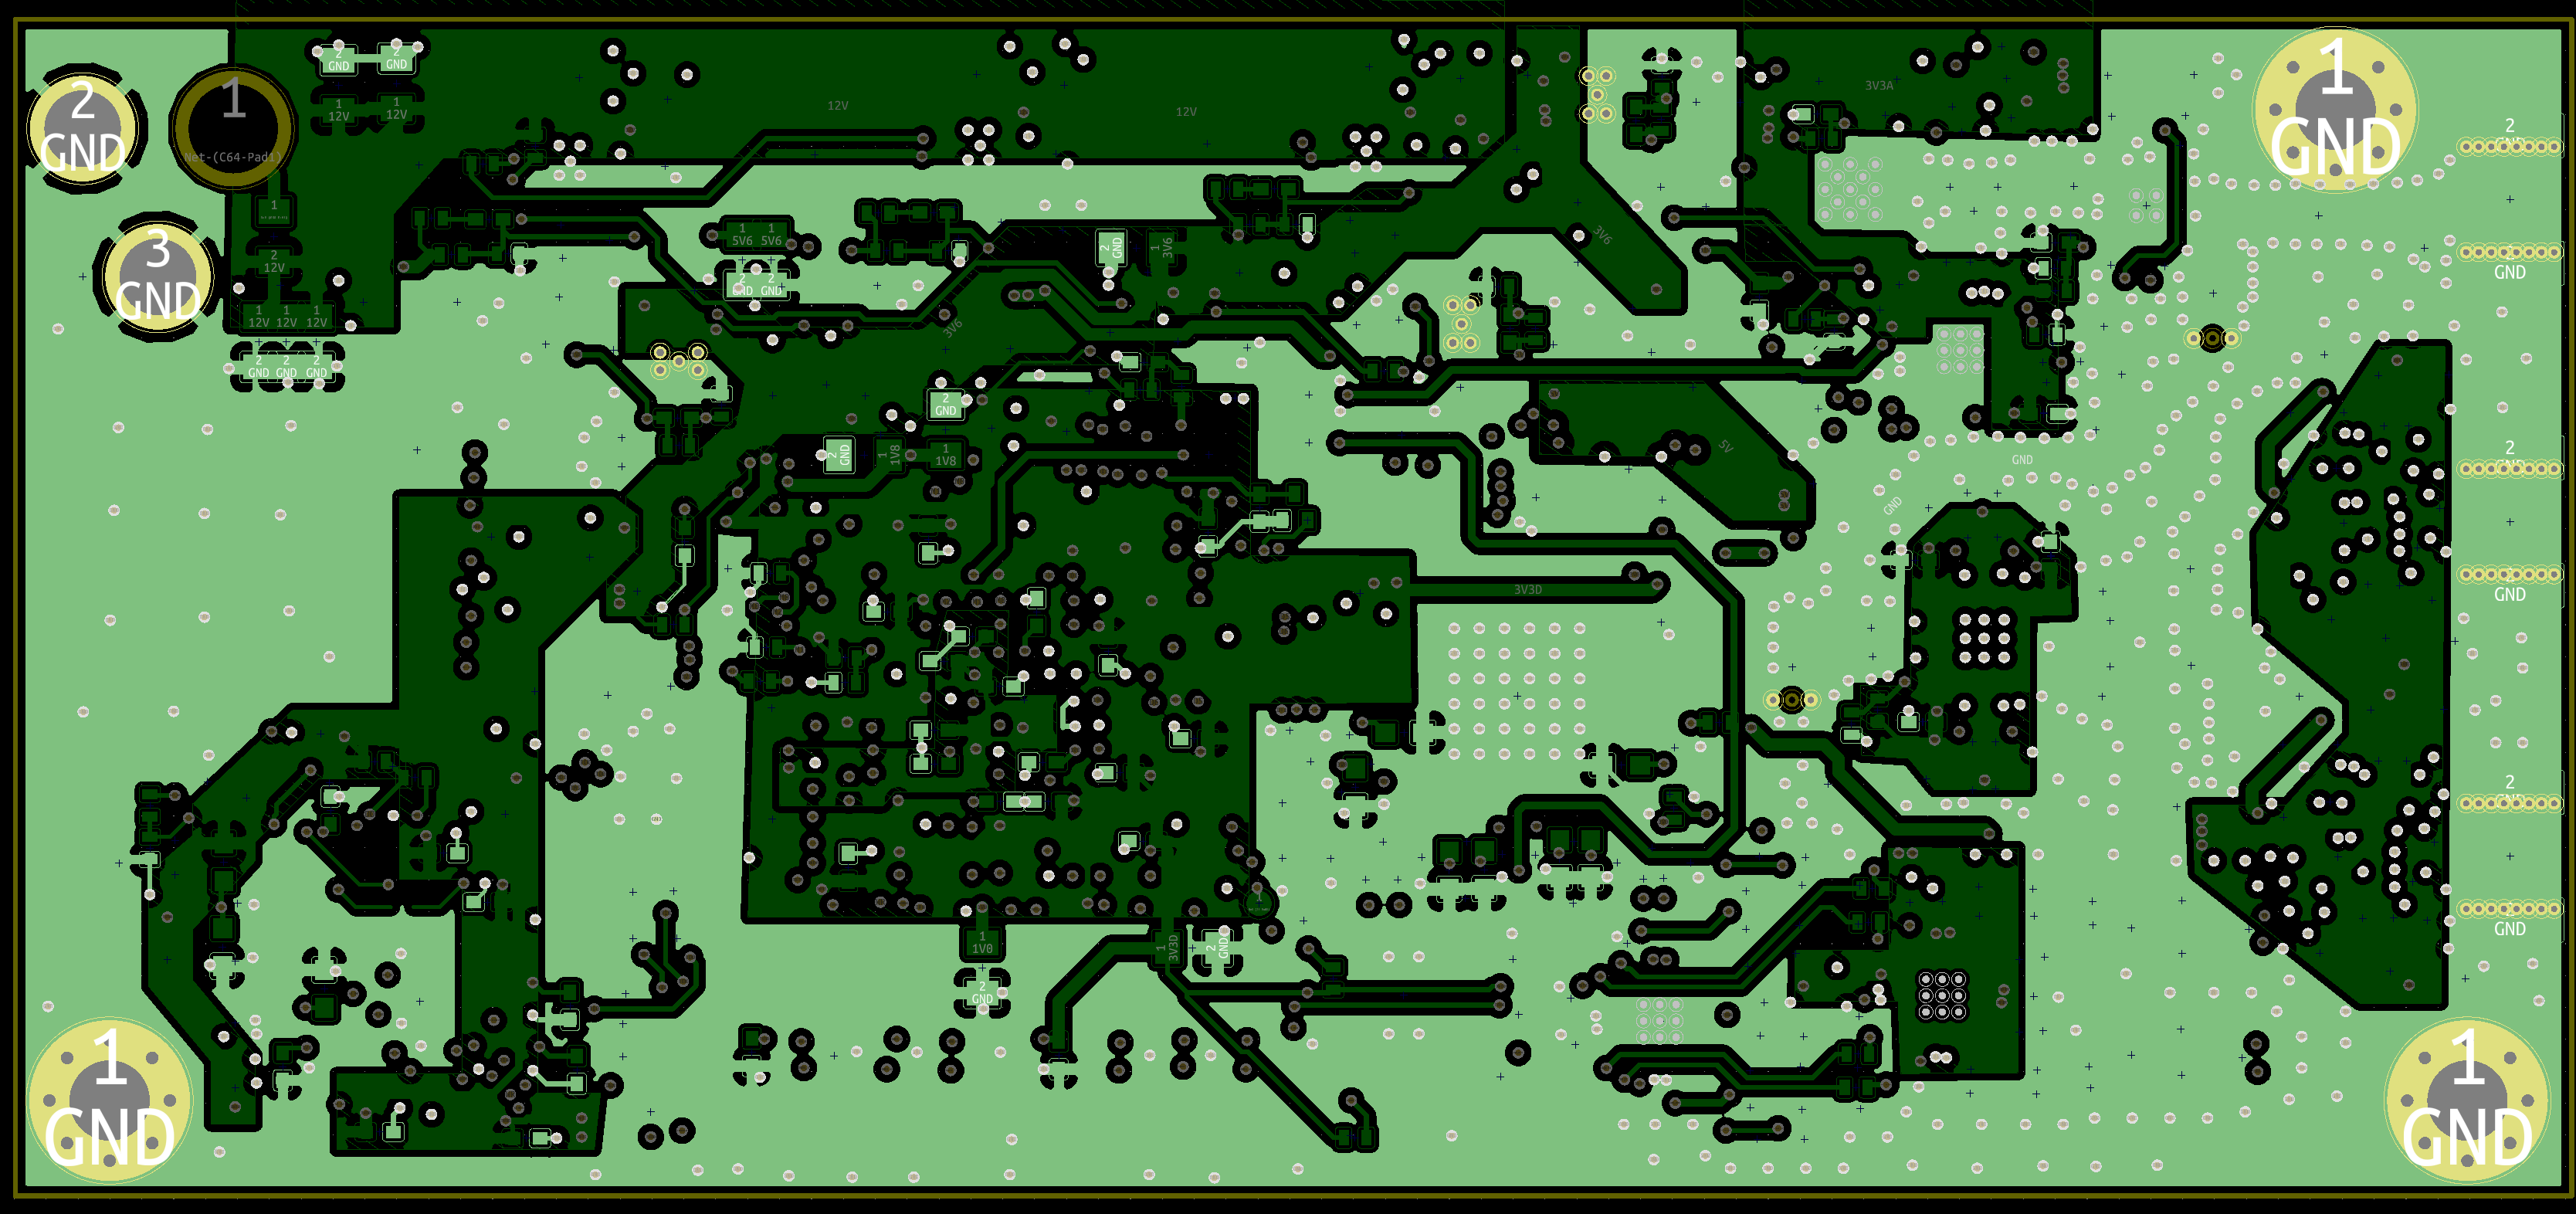
\includegraphics[width=\textwidth]{data/fmcw-layer4-gnd.png}
  \caption{The 4th layer of the PCB contains a large ground plane with many vias interspersed.}
  \label{fig:fmcw-layer4-gnd}
\end{figure}

\begin{figure}[h]
  \centering
  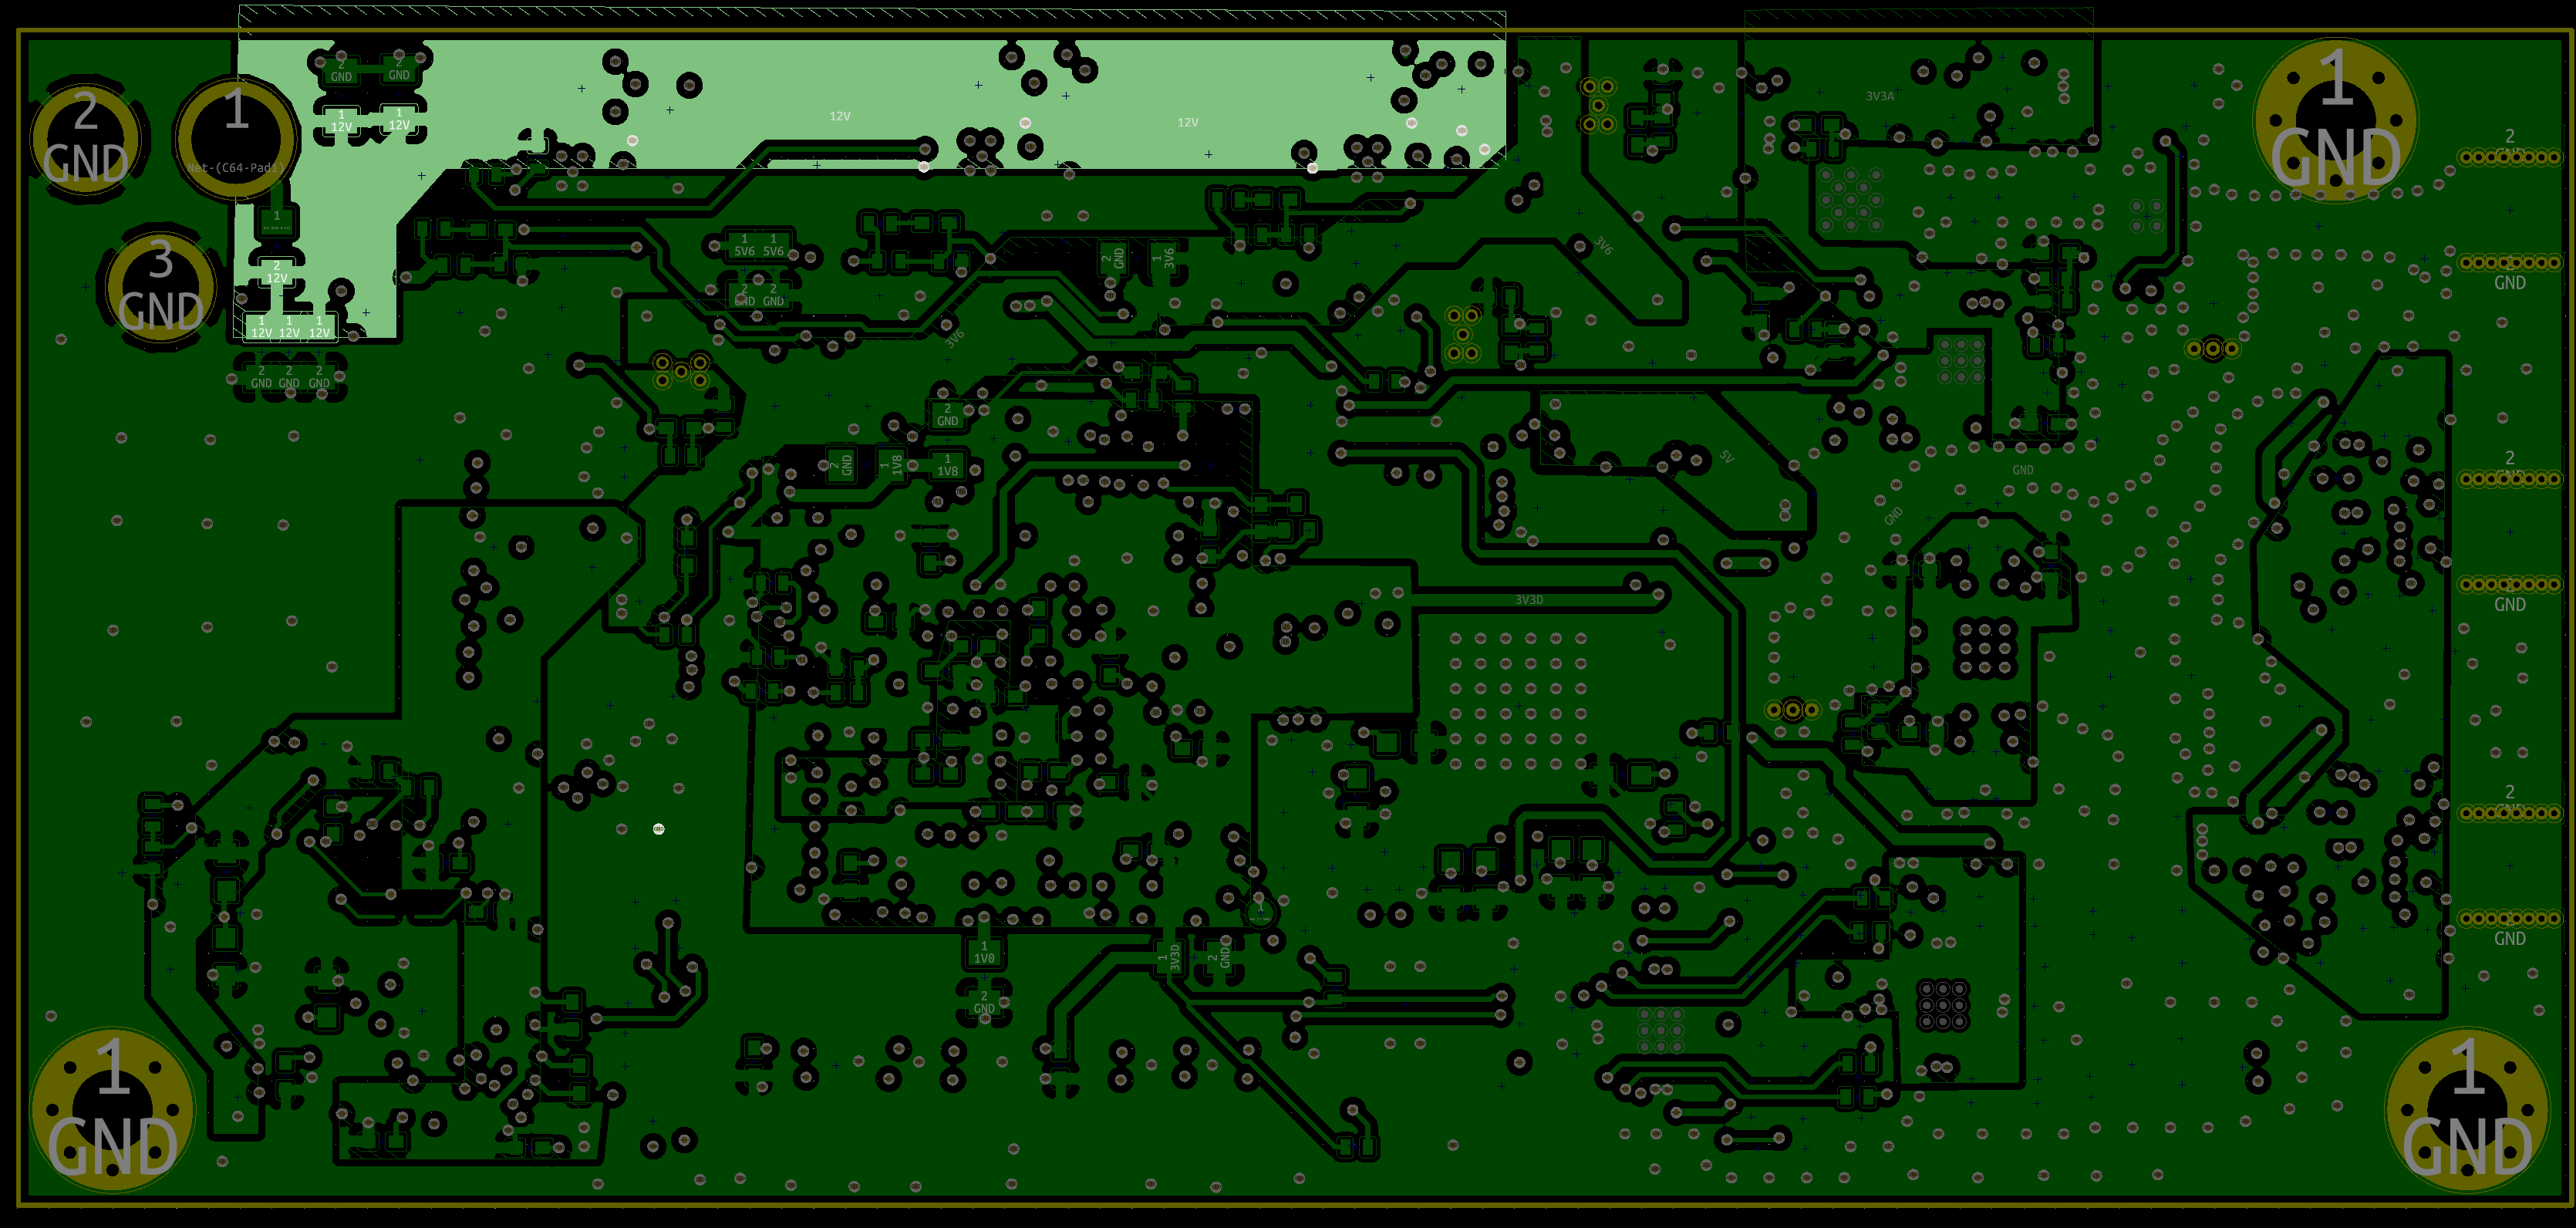
\includegraphics[width=\textwidth]{data/fmcw-layer4-12v.png}
  \caption{The 12V power plane is located at the top of the board adjacent to the D barrel jack and
    the buck converters it feeds.}
  \label{fig:fmcw-layer4-12v}
\end{figure}

\begin{figure}[h]
  \centering
  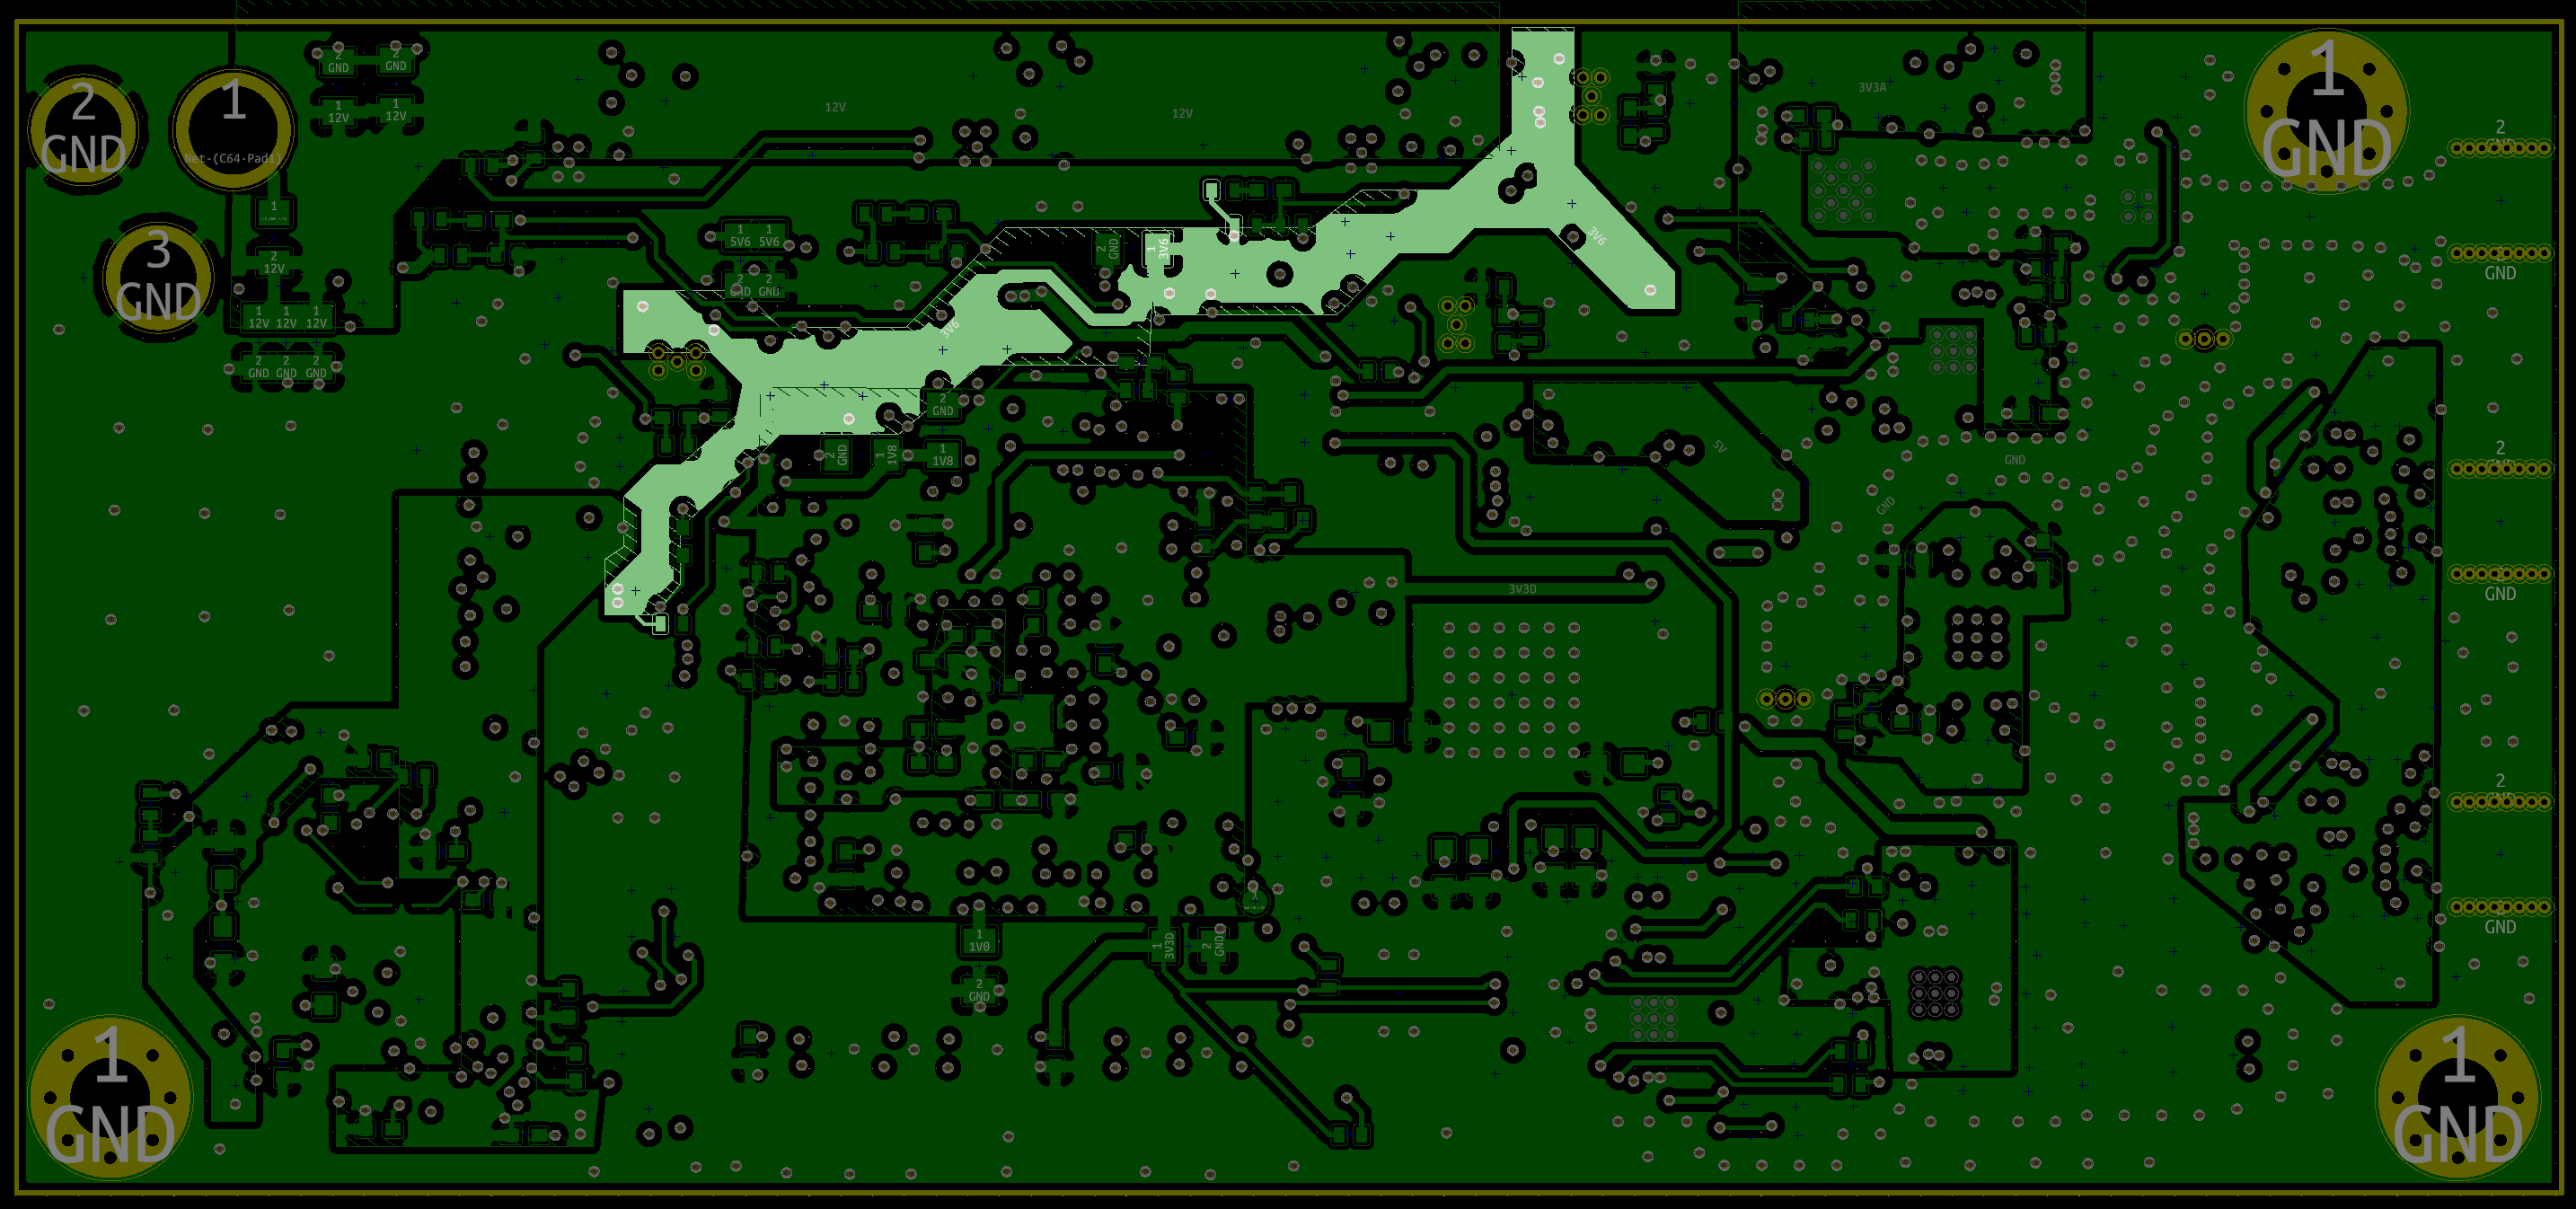
\includegraphics[width=\textwidth]{data/fmcw-layer4-3v6.png}
  \caption{There is a 3.6V power plane that is the output of one of the buck converter and is use as
    the input to several linear regulators that output 1.8V 3.0V and 3.3V.}
  \label{fig:fmcw-layer4-3v6}
\end{figure}

\begin{figure}[h]
  \centering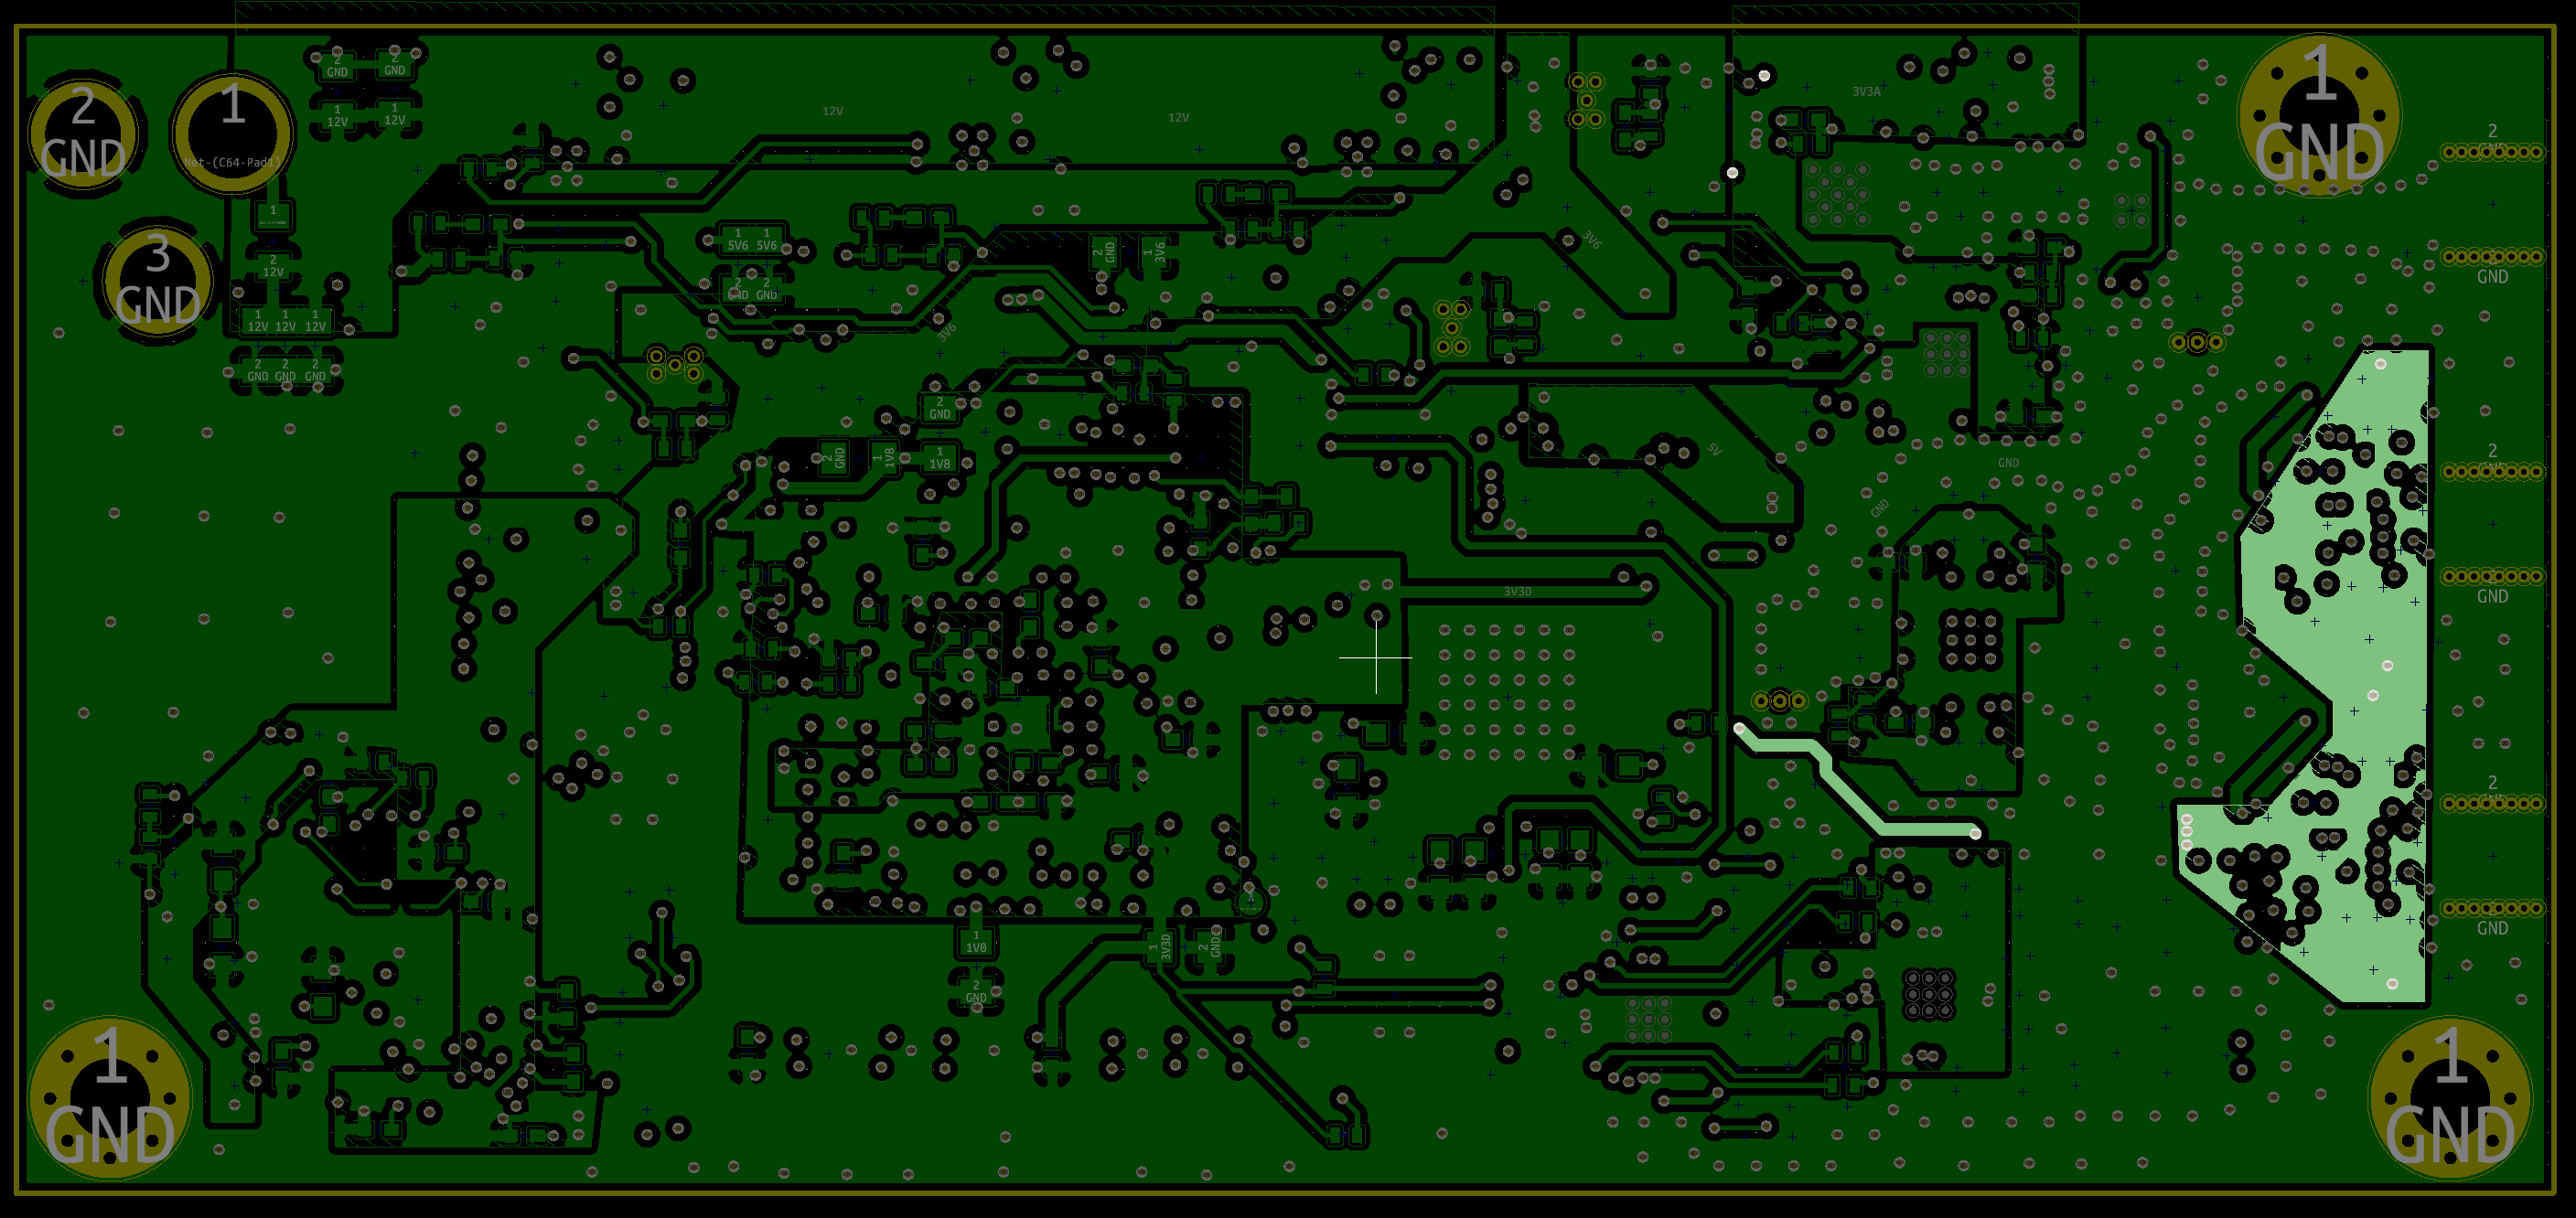
\includegraphics[width=\textwidth]{data/fmcw-layer4-3v0.png}
  \caption{A 3V power plane is used to power components near the right side of the boar (the
    righside of the board is where signal transmission and reception occur that amplify receive
    signals so they can be mixed with the transmitted signal and fed into the ADC before FPGA
    processing Notably, the 3V power plane is located near the components but far from the linear
    regulator that outputs it.}
  \label{fig:fmcw-layer4-3v0}
\end{figure}

\begin{figure}[h]
  \centering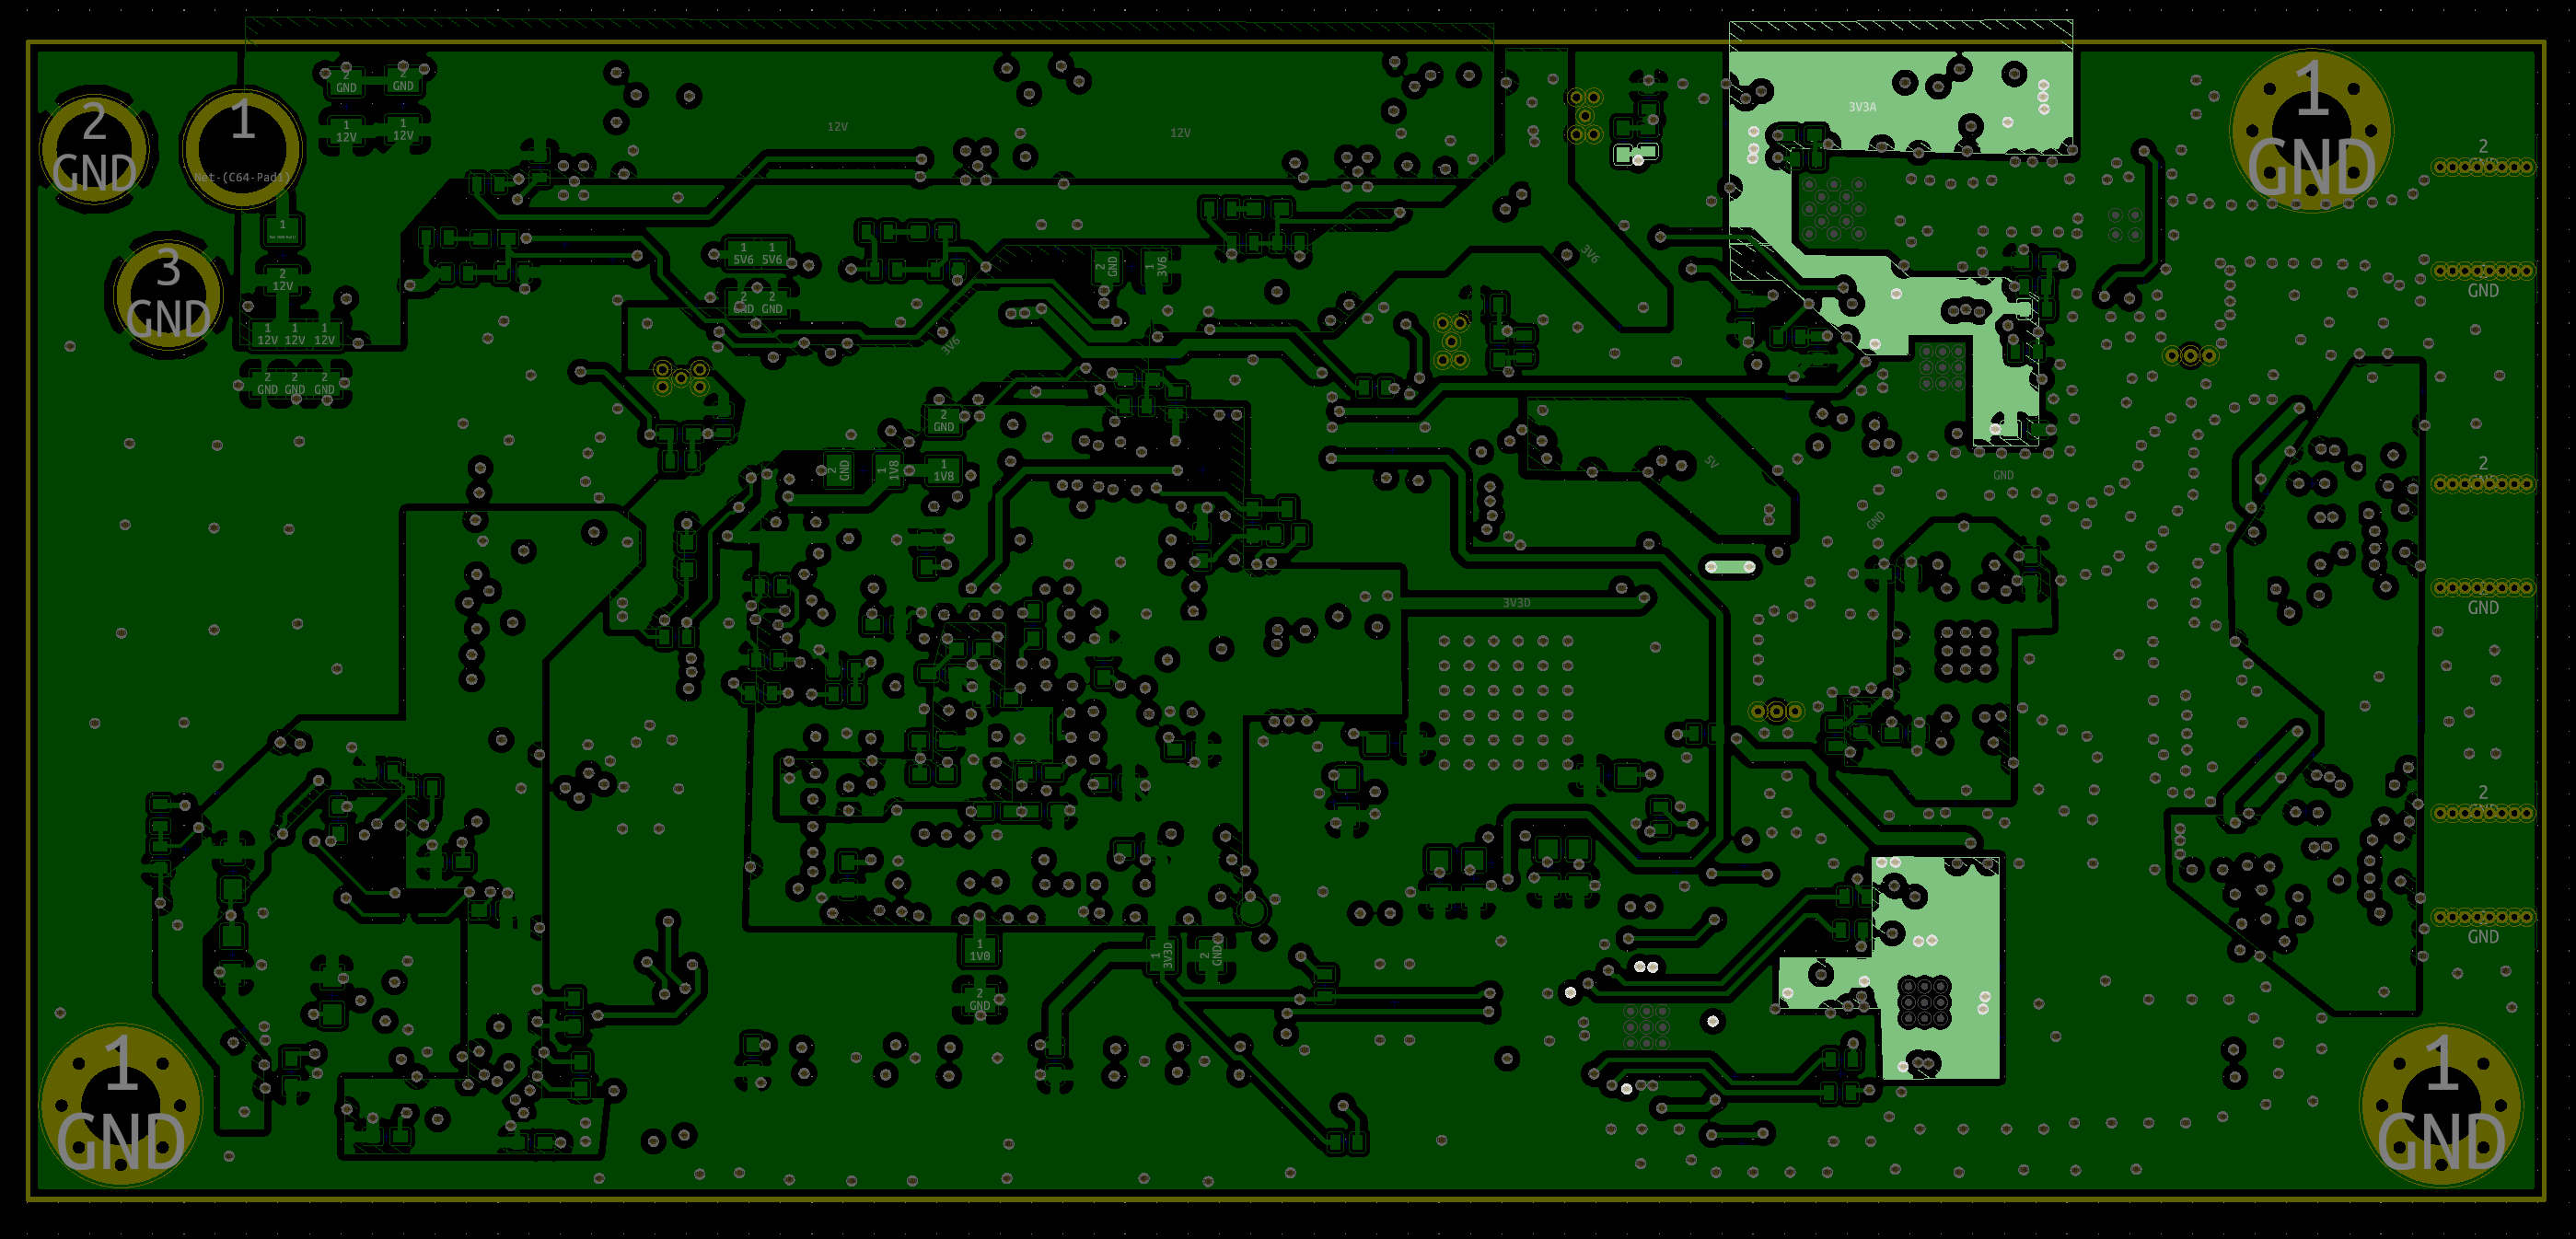
\includegraphics[width=\textwidth ]{data/fmcw-layer4-3v3a.png}
  \caption{A 3.3V power plane is used to power several components for signal transmission, such as
    a frequency synthesizer, and RF amplifier. These, along with all other reception and
    transmission circuitry, are located on the right side of the board.}
  \label{fig:fmcw-layer4-3v3a}
\end{figure}

\begin{figure}[h]
  \centering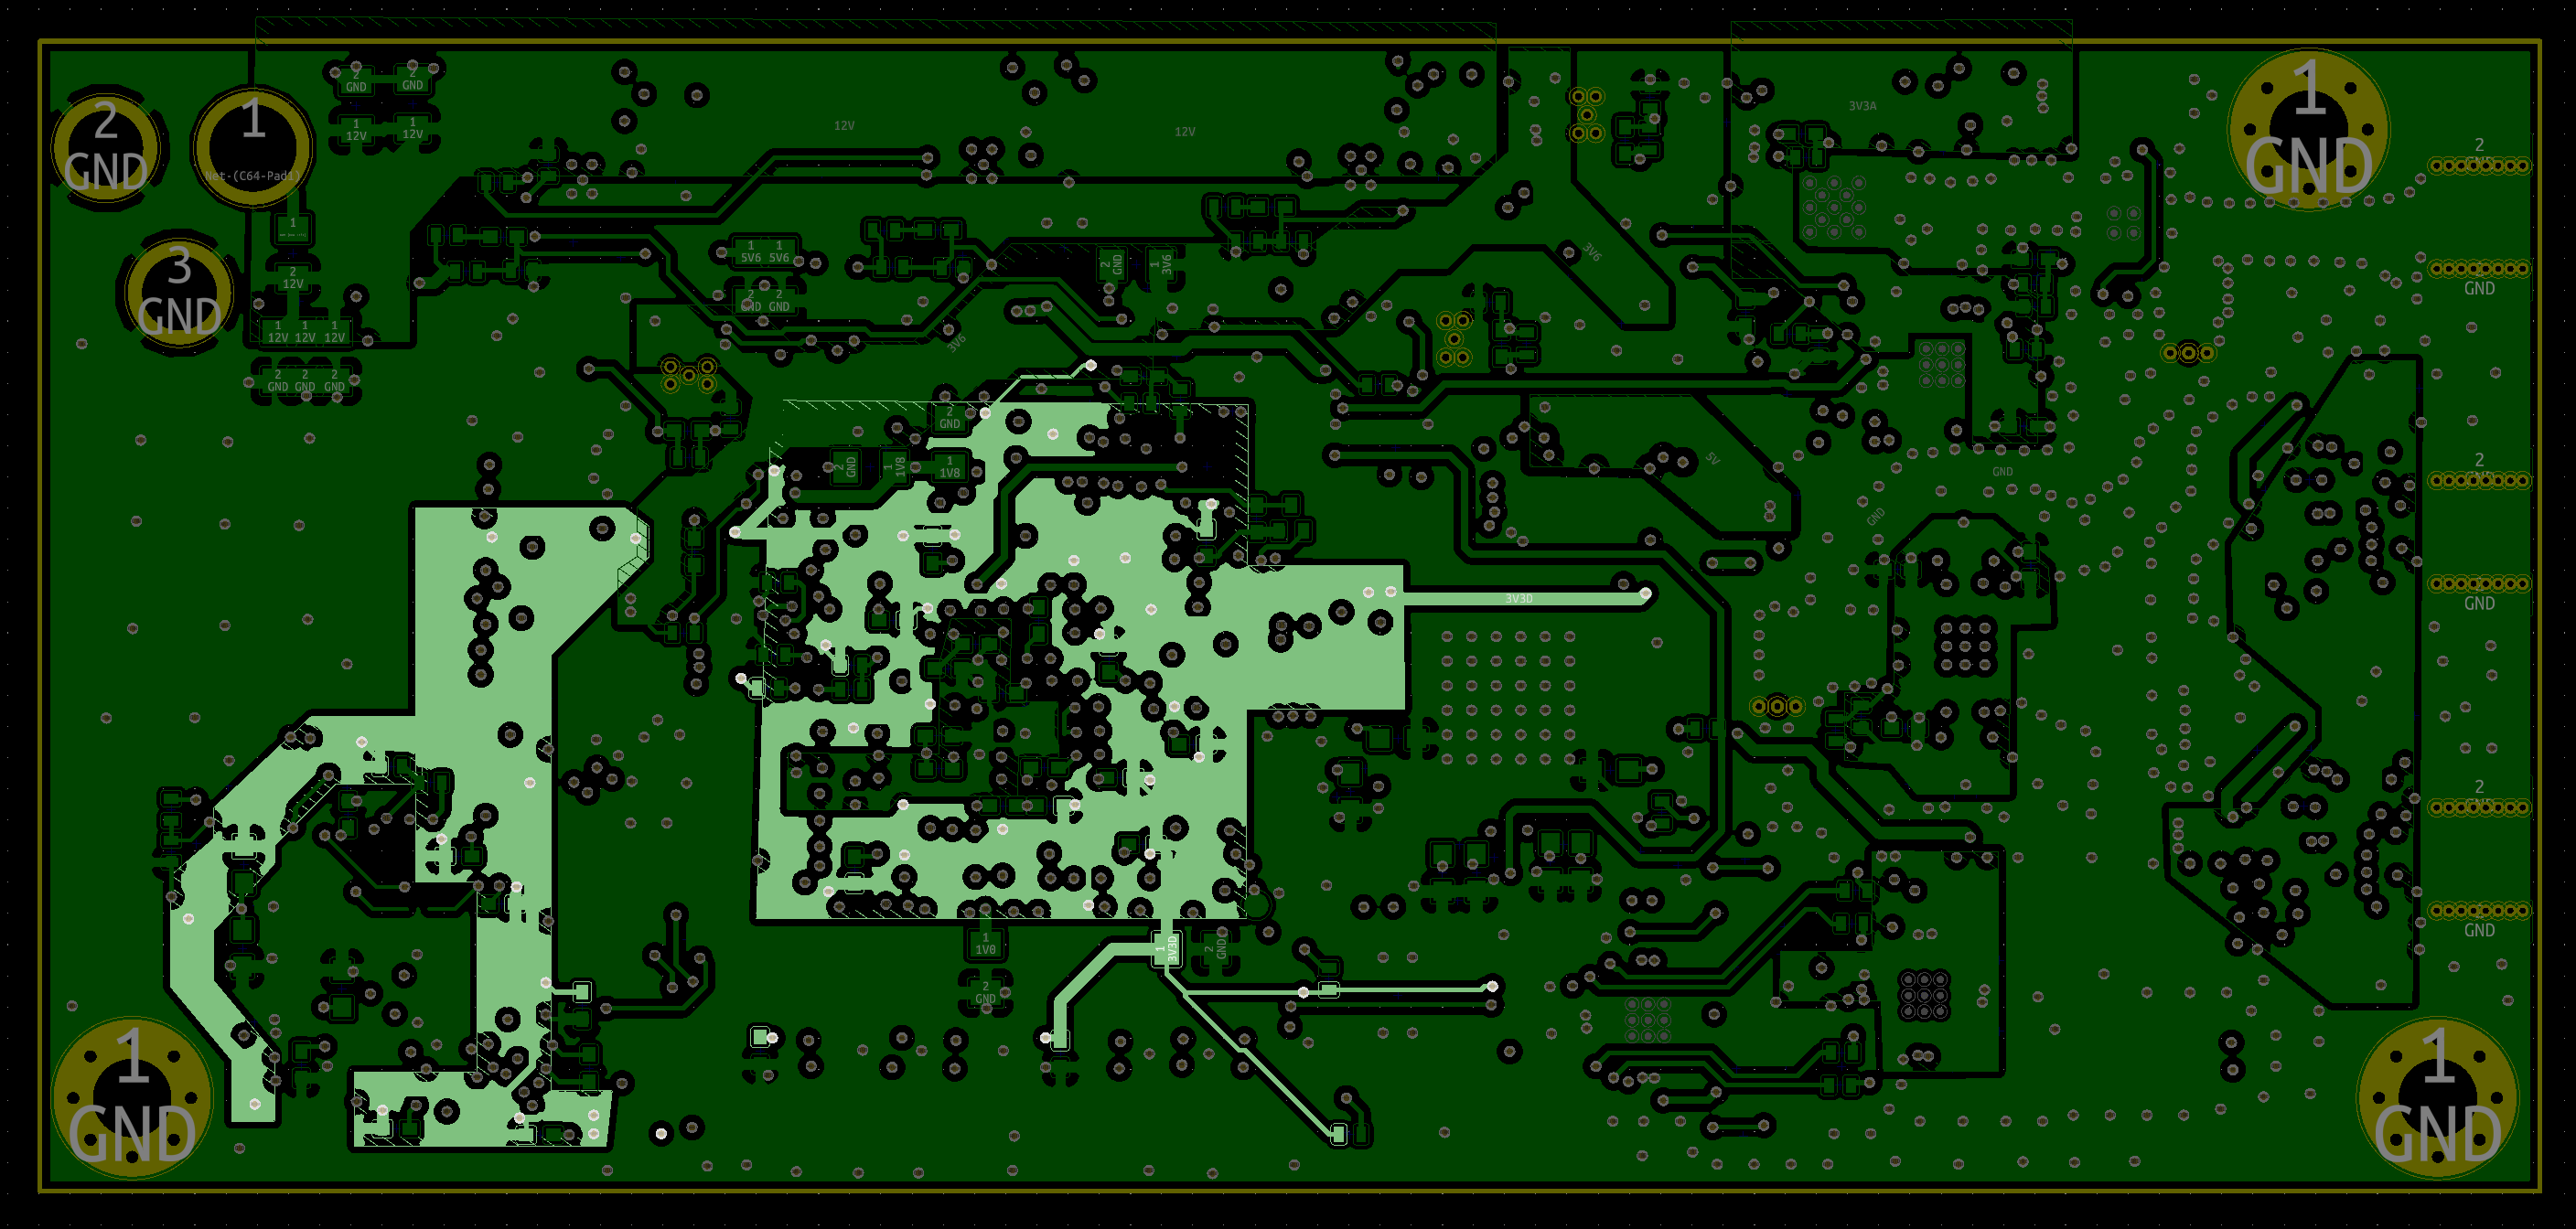
\includegraphics[width=\textwidth]{data/fmcw-layer4-3v3d.png}
  \caption{Another 3.3V power plane is used as one of the power inputs to the FPGA as well as to a
    USB-to-UART device (a configuration bit stream is sent from a host computer through a USB cable
    to the PCB where this device converts it into the proper UART format to be transmitted to
    the FPGA) and an ADC (the ADC converts the mixed transmitted-received signals to digital and
    thensends them to the FPGA for processing).}
  \label{fig:fmcw-layer4-3v3d}
\end{figure}

\begin{figure}[h]
  \centering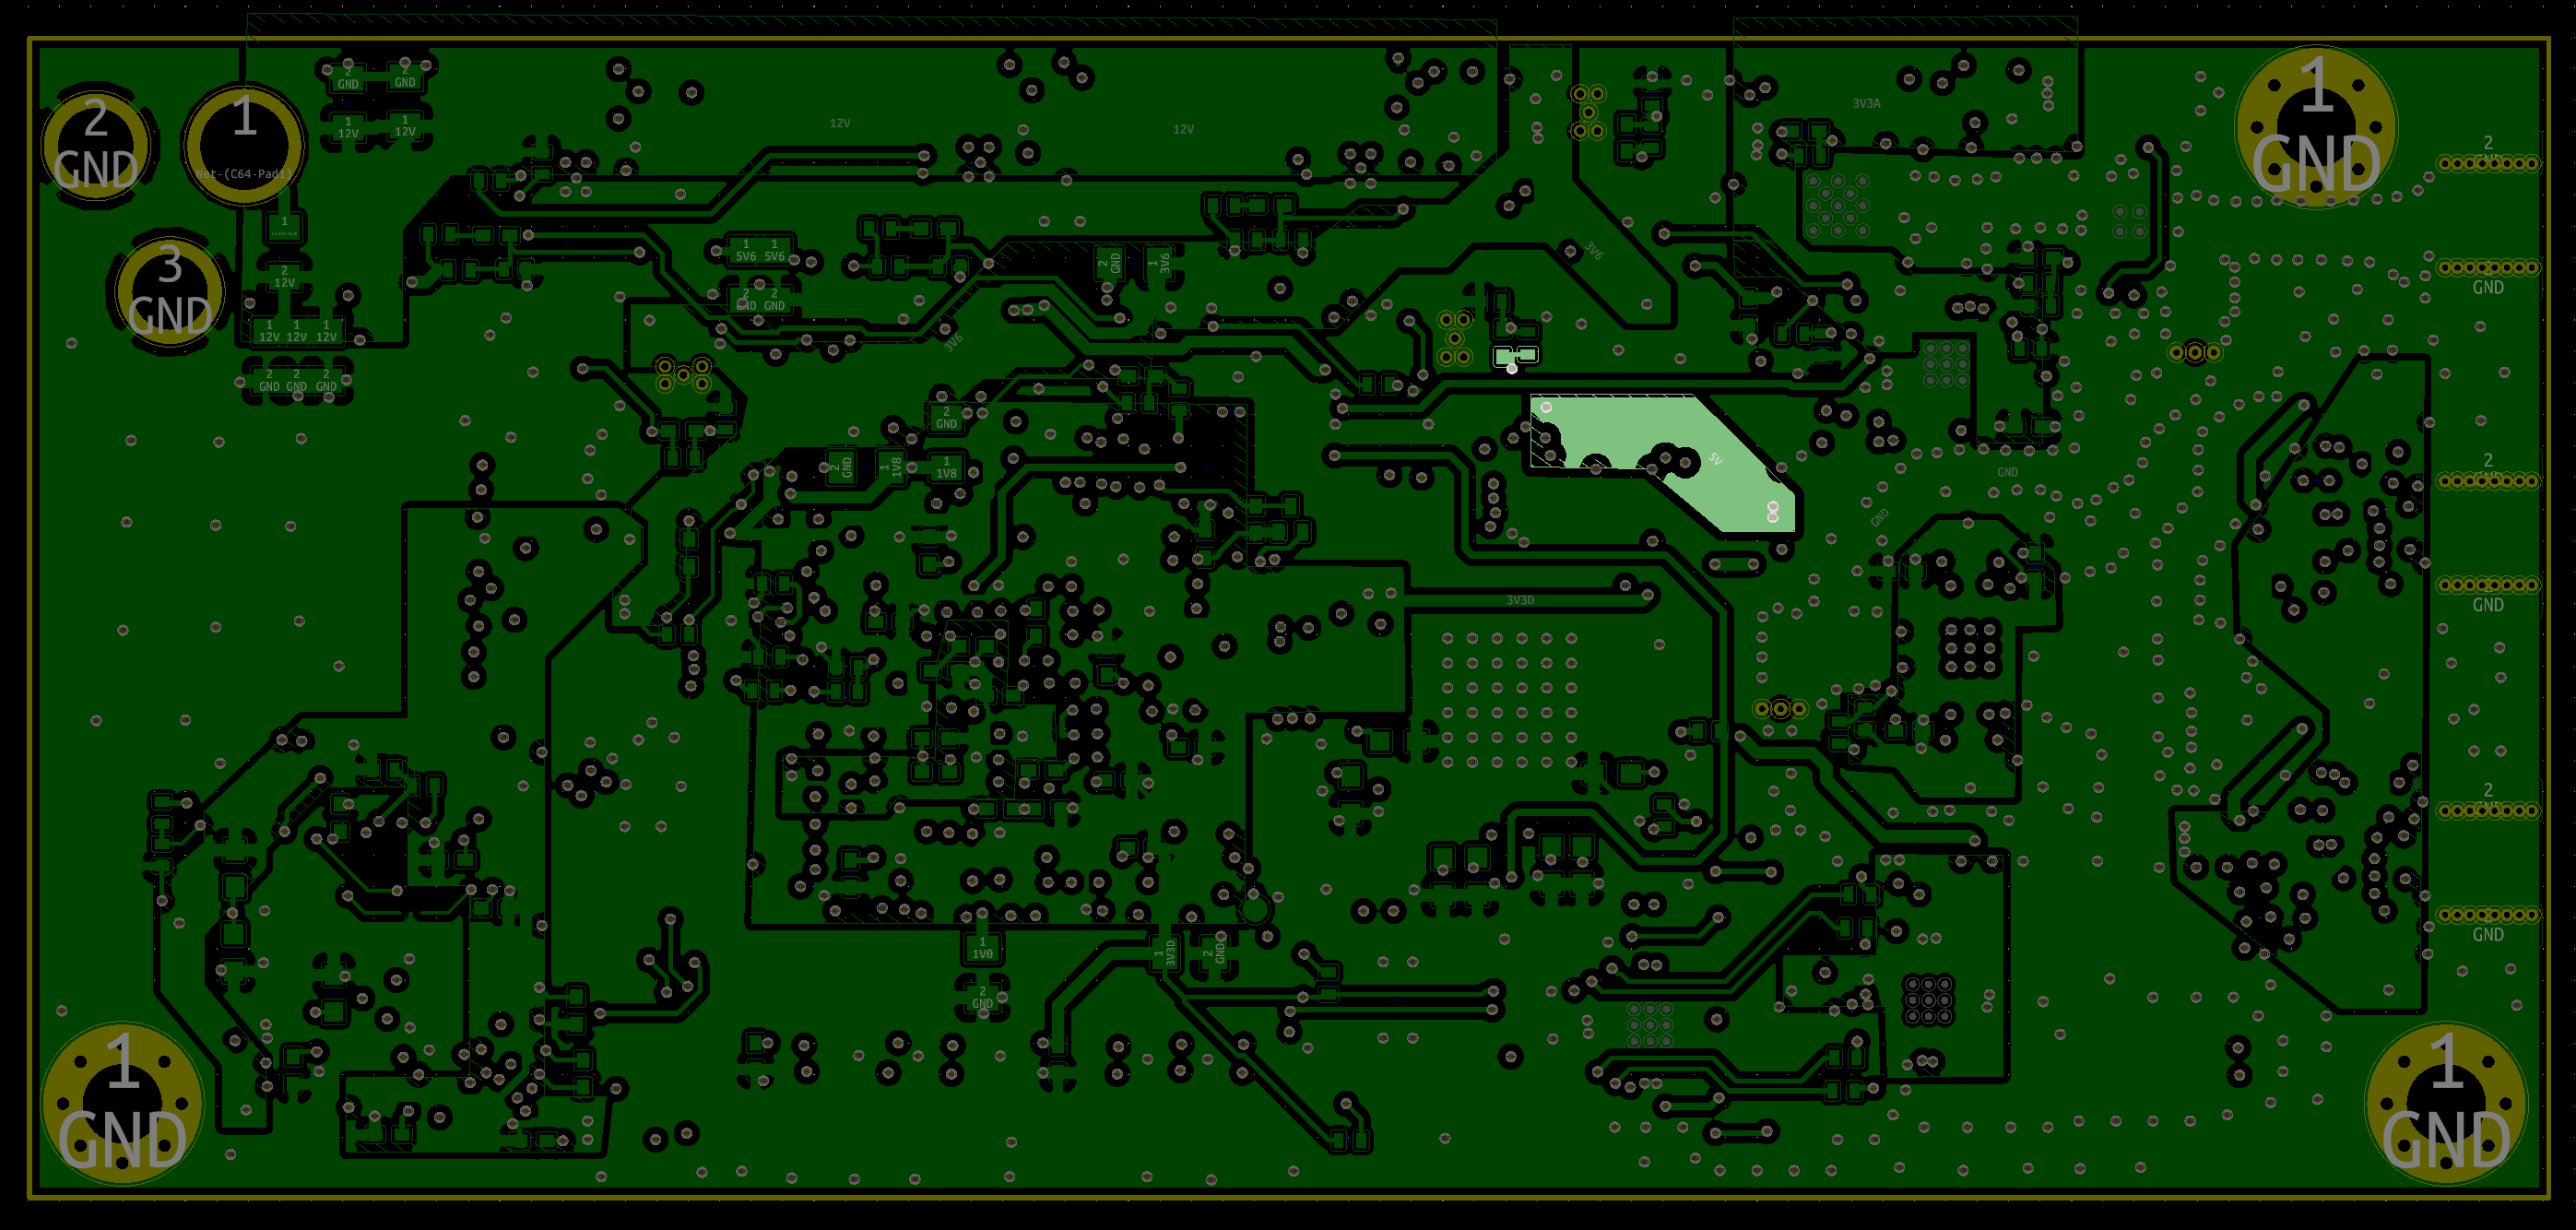
\includegraphics[width=\textwidth]{data/fmcw-layer4-5v.png}
  \caption{A 5V power plane powers one of the inputs to the frequency synthesizer for transmission.}
  \label{fig:fmcw-layer4-5v}
\end{figure}

\begin{figure}[h]
  \centering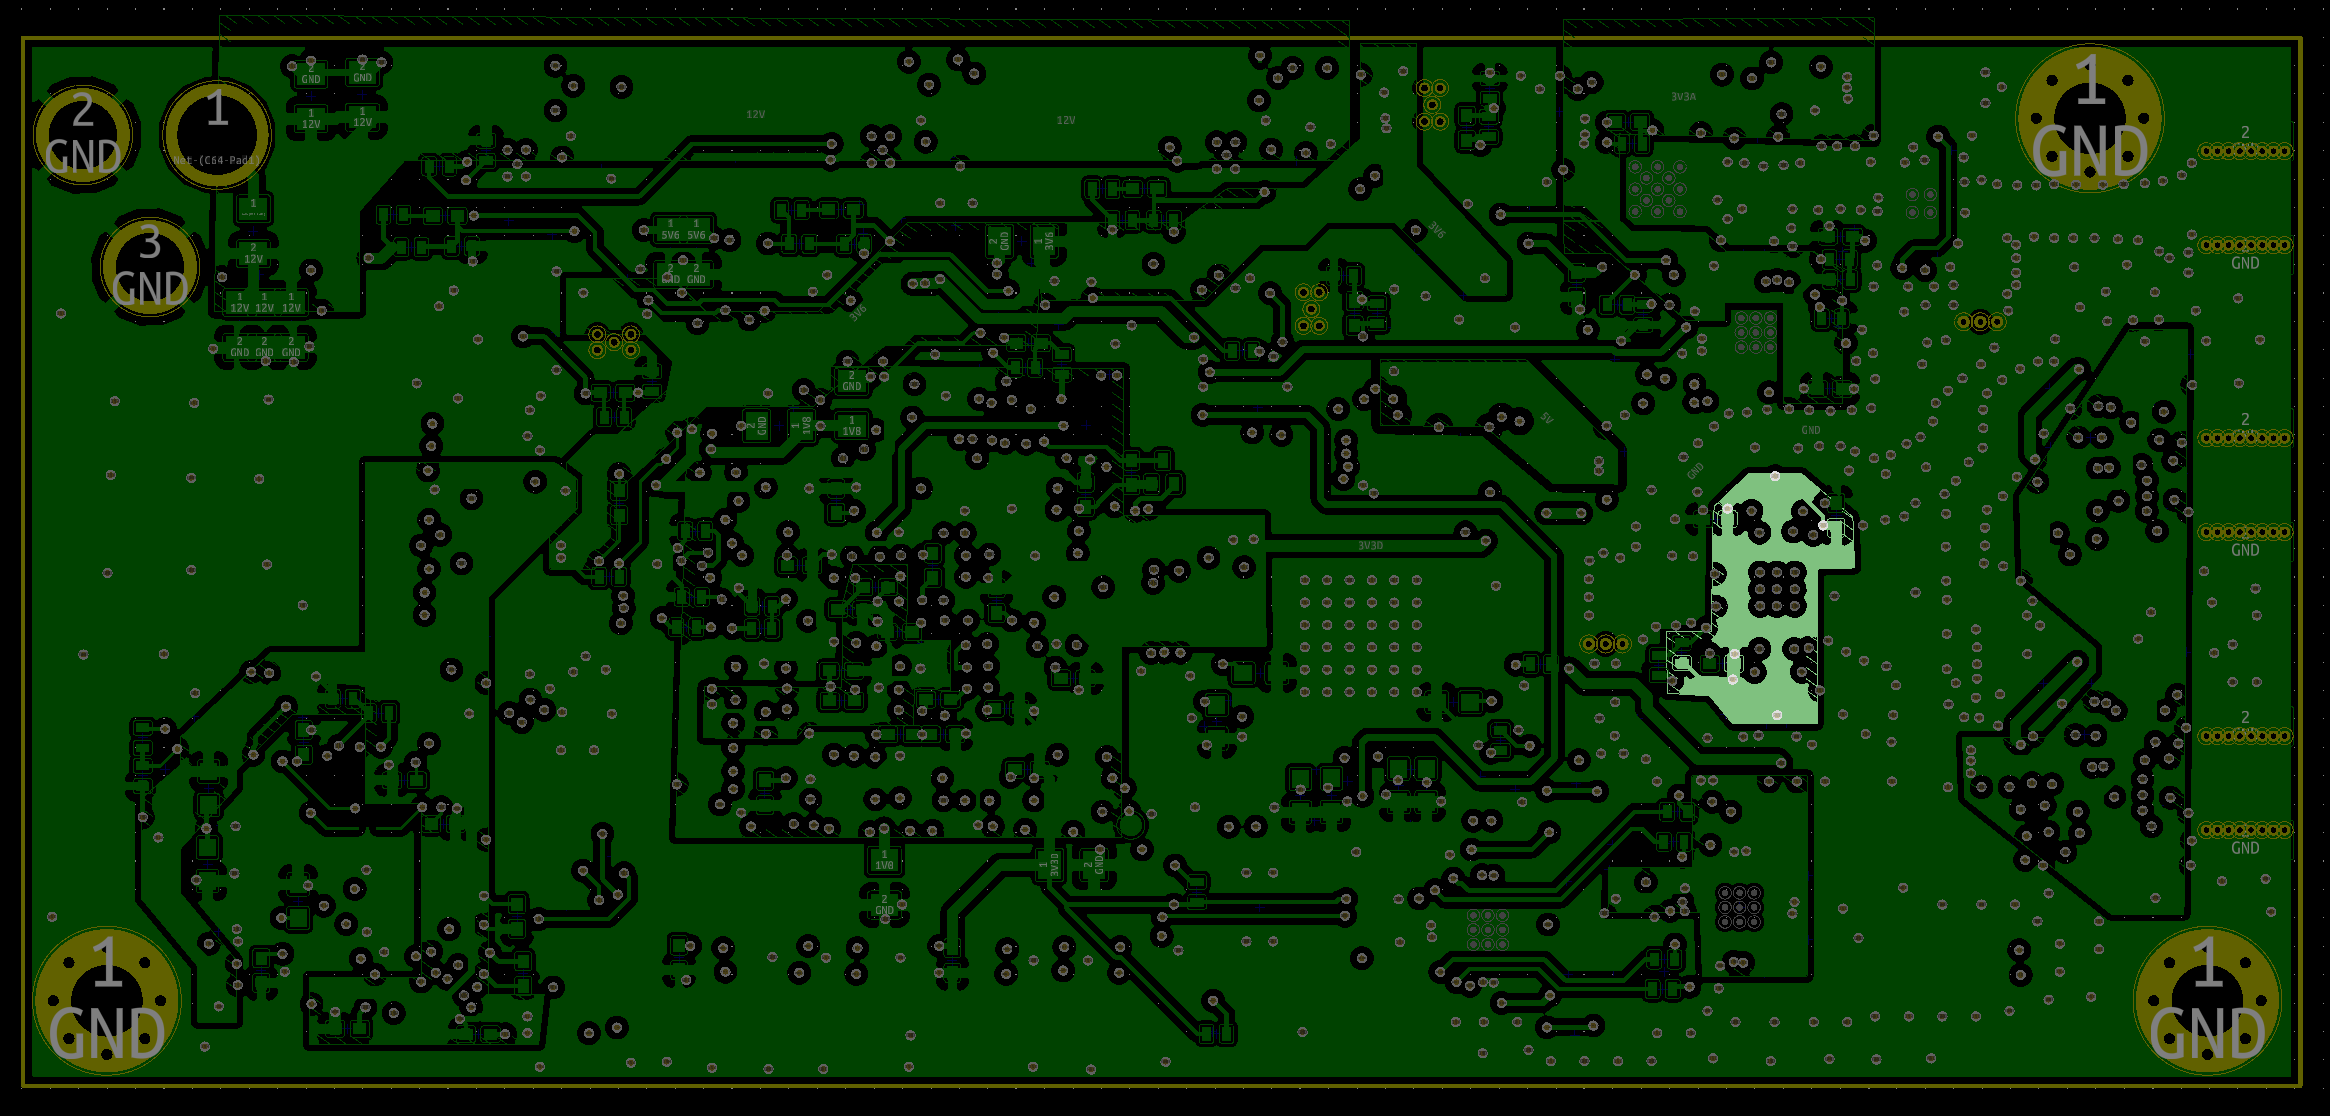
\includegraphics[width=\textwidth]{data/fmcw-layer4-5vf.png}
  \caption{Another 5V power plane is used for to power devices after going through a ferrite bead.}
  \label{fig:fmcw-layer4-5vf}
\end{figure}

\section{Component Layout Considerations}
\subsection{LTC2292 ADC}

\begin{itemize}
\item The LTC2292 contains 4 positive voltage supply pins each requiring a 0.1$\mu$F bypass
  capacitor. One capacitor each should be placed directly adjacent to each of the 4 voltage supply
  pins.
\item The device contains 2 input pins for the voltage of the device where the output data
  is sent. These, similarly require a 0.1$\mu$F capacitor each. As before they should be placed next
  to their respective pins, not next to one another.
\item VCMA and VCMB each are connected to a 2.2$\mu$F capacitor to GND. They should be placed
  as close to the pins as possible.
\item REFHA and REFLA (and REFHB and REFLB) have a 0.1$\mu$F capacitor connected between
  them. These are the most critical capacitors connected to the ADC. They must be placed 1.5mm away
  at most, and preferably closer to the pins.
\end{itemize}

\subsection{RX1 \ RX2}

\begin{itemize}
\item The 100pF capacitor used to bypass TRF37A73 should be place as close as possible to VCC.
\end{itemize}

\section{RF Impedance Matching}

The right side of the board houses the RF circuitry (i.e. transmitter, receivers and SMA
connectors). The signals are carried to the antennas (a patch-fed horn for transmission and a
patcharray for reception) via a 50$\si{\Omega}$ coaxial cable. All RF inputs and outputs for
components should match this 50$\si{\Omega}$ impedance. The original layout does not seem overly
concerned with the microstrip transmission line width between RF components. They are kept short and
generally have a trace width of about 0.3mm. However, many of them are not even remotely straight
and this doesn't seem to be an issue. Where possible the microstrips should be kept short, straight
and with an unbroken ground plane beneath them. That seems to be all that is necessary for
impedancematching. The patch antennas however will need to be appropriately hooked up in order to
match the50$\si{\Omega}$ impedance. This should be a relatively straightforward calculation. The
setup Henrik uses seems to be the most logical one. He uses a single patch-fed horn antenna for
transmission anda patch array for reception. The horn antenna is made of thin copper. More
sophisticated horn antennas require the ability to weld and probably modeling software (e.g. CST).

\chapter{Full Schematic}
\label{cha:schematic}

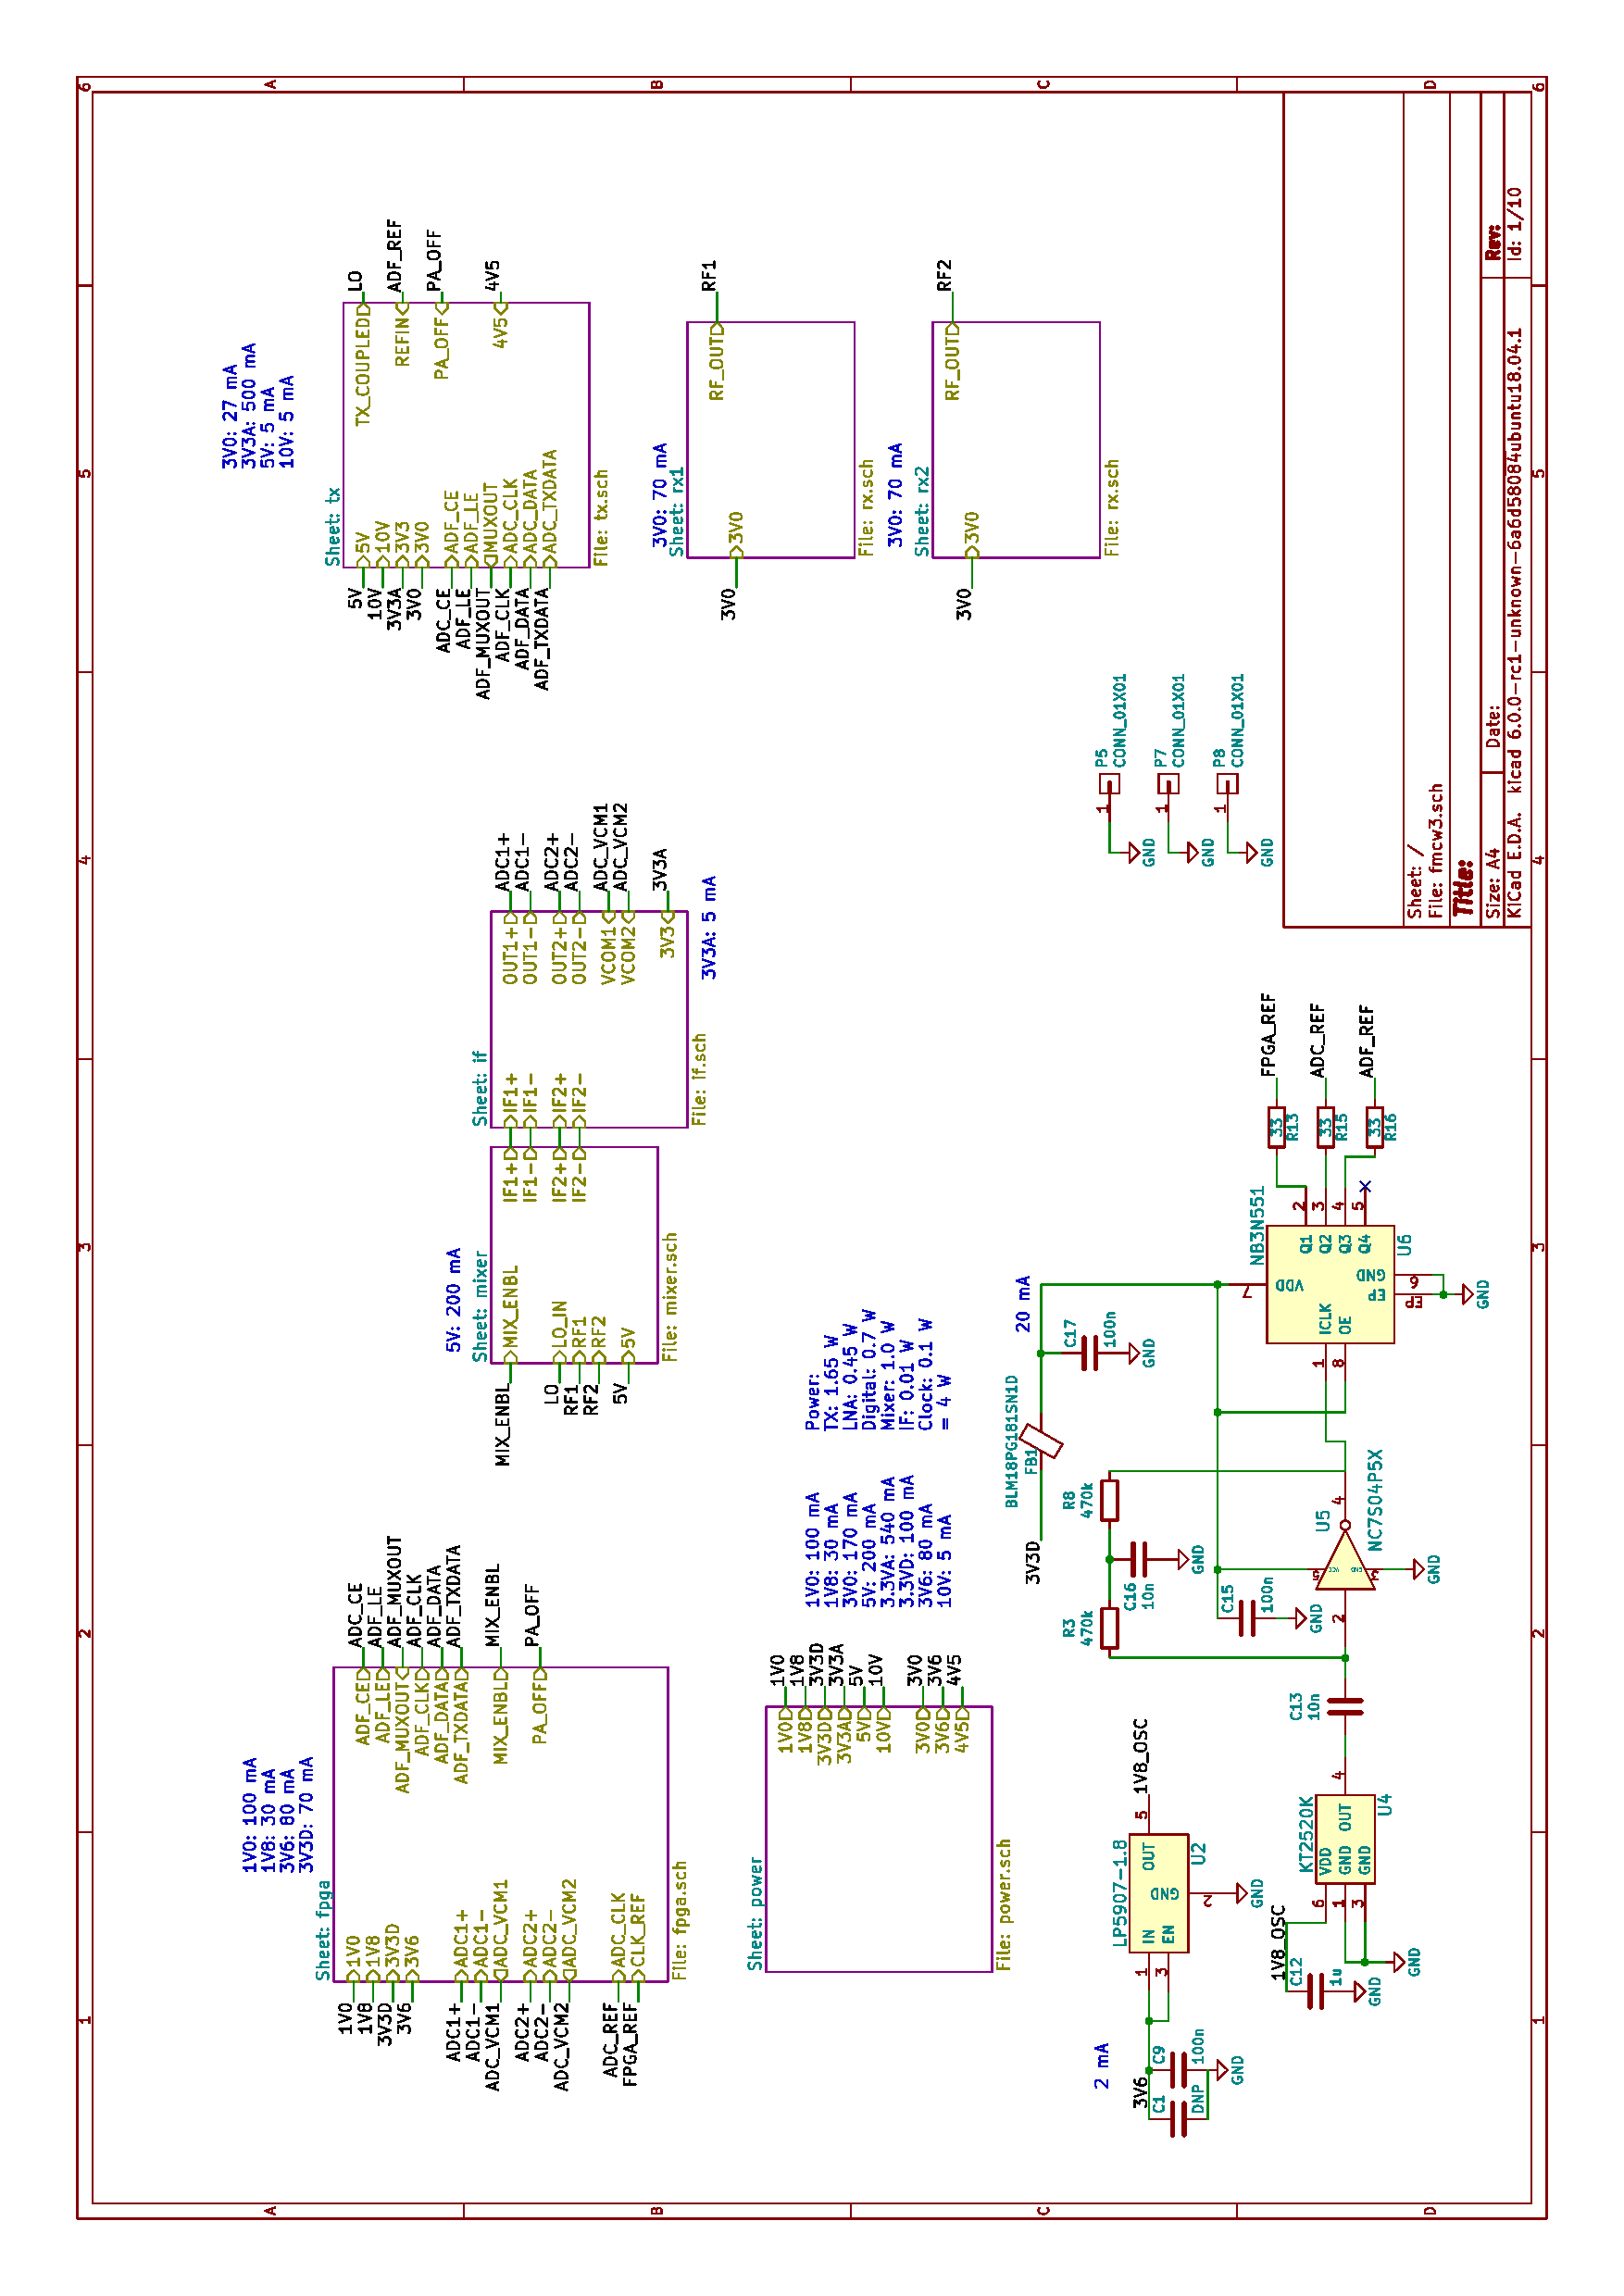
\includepdf[pages=-, landscape=true, angle=-90]{data/fmcw-schematic.pdf}

\end{document}